\documentclass[a4paper,12pt,twoside]{book}
\usepackage{upatras-thesis}

% PDF settings
%
\hypersetup
{
    pdfauthor={\me},
    pdftitle={\shortdoctitle},
    pdfsubject={\doctitle},
    pdfkeywords={\keywords},
    pdfproducer={pdfLaTeX},
    pdfcreator={\creator}
}

%
% These commands need to be defined in order to produce a correct and personalized document
%

%%%%%%%%%%%%%% English
\newcommand{\shortdoctitle}{Diploma Thesis}
\newcommand{\doctitle}{Software/Hardware Co-design and FPGA Implementation of the Security Protocol IPSec for the Internet Protocol version 6 (IPv6)}
\newcommand{\docsubtitle}{Υπότιτλος εγγράφου}
\newcommand{\division}{Electronics \& Computers}
\newcommand{\lab}{Very Large Scale of Integration LAB (VLSI Design)}

\newcommand{\me}{Georgios Gkitsas} %(σε γενική πτώση) ΠΡΟΣΟΧΗ: στοιχεία σε γενική πτώση. Παράδειγμα: Άγγελου Σικελιανού του Ιωάννη
%
\newcommand{\nomme}{Georgios Gkitsas} %(σε ονομαστική πτώση) ΠΡΟΣΟΧΗ: στοιχεία σε ονομαστική πτώση. Παράδειγμα: Άγγελος Σικελιανός του Ιωάννη
%
\newcommand{\studnum}{6732}
\newcommand{\keywords}{Λέξεις Κλειδιά}
\newcommand{\monthyear}{ 31 March 2014}

\newcommand{\supname}{Georgios Theodoridis}
\newcommand{\suptitle}{Assistant Professor}
\newcommand{\supuni}{}

\newcommand{\cosupname}{Συνεπιβλέποντας Καθηγητής}
\newcommand{\cosuptitle}{Τίτλος Συνεπιβλέποντα Καθηγητή}
\newcommand{\cosupuni}{}

\newcommand{\headofdivision}{Housos Efthymios}
\newcommand{\headofdivisiontitle}{Professor}

%%%%%%%%%%%%%% Greek
% \newcommand{\shortdoctitle}{Διπλωματική Εργασία}
% \newcommand{\doctitle}{Συ-σχεδίαση Υλικού/Λογισμικού και Υλοποίηση σε πλατφόρμα FPGA του πρωτοκόλλου ασφαλείας IPsec για το Internet Protocol version 6 (IPv6)}
% \newcommand{\docsubtitle}{Υπότιτλος εγγράφου}
% \newcommand{\division}{Ηλεκτρονικής και Υπολογιστών}
% \newcommand{\lab}{Εργαστήριο Σχεδιασμου Ολοκληρωμένων Κυκλωμάτων
% Μεγάλης Κλίμακας\\(VLSI Design)}

% \newcommand{\me}{Γεώργιου Γκίτσα του Χρήστου} %(σε γενική πτώση) ΠΡΟΣΟΧΗ: στοιχεία σε γενική πτώση. Παράδειγμα: Άγγελου Σικελιανού του Ιωάννη
% %
% \newcommand{\nomme}{Γεώργιος Γκίτσας του Χρήστου} %(σε ονομαστική πτώση) ΠΡΟΣΟΧΗ: στοιχεία σε ονομαστική πτώση. Παράδειγμα: Άγγελος Σικελιανός του Ιωάννη
% %
% \newcommand{\studnum}{6732}
% \newcommand{\keywords}{Λέξεις Κλειδιά}
% \newcommand{\monthyear}{ 31 Μαρτίου 2014}

% \newcommand{\supname}{Γεώργιος Θεοδωρίδης}
% \newcommand{\suptitle}{Επίκουρος Καθηγητής}
% \newcommand{\supuni}{}

% \newcommand{\cosupname}{Συνεπιβλέποντας Καθηγητής}
% \newcommand{\cosuptitle}{Τίτλος Συνεπιβλέποντα Καθηγητή}
% \newcommand{\cosupuni}{}

% \newcommand{\headofdivision}{Χούσος Ευθύμιος}
% \newcommand{\headofdivisiontitle}{Καθηγητής}

%%%%%%%%%%%%%%%%%%%%%%%%%%%%%%%%%%%%%%%%%%%%%%%%%%%%%%%%%%%%%%
\newcommand{\ts}{\textsuperscript}
\newcommand{\ssc}{\textsubscript}
\newdimen{\algindent}
\setlength\algindent{1.5em}          % algorithmic indent=1.5em
\algnewcommand\LeftComment[2]{%
\hspace{#1\algindent}$\triangleright$ \eqparbox{COMMENT}{#2} \hfill %
}

\definecolor{bluekeywords}{rgb}{0.13,0.13,1}
\definecolor{greencomments}{rgb}{0,0.5,0}
\definecolor{redstrings}{rgb}{0.9,0,0}

\lstdefinestyle{mycodestyle}{language=C,
    basicstyle=\small\ttfamily,
    showstringspaces=false,
    breaklines=true,
    frameround=ffff,
    frame=single,
    rulecolor=\color{black},
    autogobble=true
    commentstyle=\color{greencomments},
    keywordstyle=\color{bluekeywords},
    stringstyle=\color{redstrings},
    tabsize=2,
    captionpos=b, 
    commentstyle=\color{mygreen},
    morekeywords={err_t, require, end, in},            % if you want to add more keywords to the set
}


\author{\me}

% GLOSSARY
\makeglossaries
\newglossaryentry{parallax}
{
    % name=Parallax,
    % description={is a dispacement in the apparent position of an object viewed along two different lines of sight.}
}


% BEGIN DOCUMENT
\begin{document}

% SET PAGE NUMBERING TO ROMAN
\pagenumbering{roman}
\setcounter{page}{3}

%*************************%
%         TITLES          %
%*************************%

% \begin{titlepage}
% \begin{center}
% % Upper part of the page
% {\large ΠΑΝΕΠΙΣΤΗΜΙΟ ΠΑΤΡΩΝ - ΠΟΛΥΤΕΧΝΙΚΗ ΣΧΟΛΗ}\\
% \large ΤΜΗΜΑ ΗΛΕΚΤΡΟΛΟΓΩΝ ΜΗΧΑΝΙΚΩΝ\\ΚΑΙ ΤΕΧΝΟΛΟΓΙΑΣ ΥΠΟΛΟΓΙΣΤΩΝ\\
% \hfill \break
% 
\includegraphics[width= 0.8\textwidth]{up_landscape}\\
% \hfill \break
% {\Large Τομέας: \division \\
% Εργαστήριο: \lab }\\[1cm]

% {\uline{\LARGE{\shortdoctitle }}}\\ [0.5cm]
% του φοιτητή του Τμήματος Ηλεκτρολόγων Μηχανικών και Τεχνολογίας\\
% Υπολογιστών της Πολυτεχνικής Σχολής  του Πανεπιστημίου Πατρών\\[1cm]

% {\LARGE \me }\\[0.5cm]
% {\Large αριθμός μητρώου: \studnum}\\[1cm]

% \uline{\large Θέμα}\\[0.5cm]
% \textbf{\large \doctitle }\\[1cm]
% \uline{\large Επιβλέπων}\\[0.5cm]
% % \large \suptitle \, \supname, \supuni \\[1cm]
% \large \suptitle \, \supname \\[1cm]
% \large{Αριθμός Διπλωματικής Εργασίας: }%\hspace{3cm}
% \vfill
% % Bottom of the page
% \large{Πάτρα, \monthyear}
% \end{center}
% \end{titlepage}


\begin{titlepage}
\begin{center}
% Upper part of the page
{\large UNIVERSITY OF PATRAS - SCHOOL OF ENGINEERING}\\
\large DEPARTMENT OF ELECTRICAL\\AND COMPUTER ENGINEERING\\
\hfill \break

\includegraphics[width= 0.8\textwidth]{up_landscape}\\
\hfill \break
{\Large Division: \division \\
Lab: \lab }\\[1cm]

{\uline{\LARGE{\shortdoctitle }}}\\ [0.5cm]
of the undergraduate student of the Department of Electrical and Computer \\Engineering of the School of Engineering of the University of Patras\\[1cm]
% του φοιτητή του Τμήματος Ηλεκτρολόγων Μηχανικών και Τεχνολογίας\\
% Υπολογιστών της Πολυτεχνικής Σχολής  του Πανεπιστημίου Πατρών\\[1cm]

{\LARGE \me }\\[0.5cm]
{\Large Registration number: \studnum}\\[1cm]

\uline{\large Title}\\[0.5cm]
\textbf{\large \doctitle }\\[1cm]
\uline{\large Advisor}\\[0.5cm]
% \large \suptitle \, \supname, \supuni \\[1cm]
\large \suptitle \, \supname \\[1cm]
\large{Thesis Number: }%\hspace{3cm}
\vfill
% Bottom of the page
\large{Patra,\monthyear}
\end{center}
\end{titlepage}
\clearemptydoublepage

% \pagestyle{empty}
\begin{center}
{\LARGE ΠΙΣΤΟΠΟΙΗΣΗ\\[1cm]}
\large Πιστοποιείται ότι η διπλωματική εργασία με θέμα\\[1cm]
\textbf{\large \doctitle }\\[1cm]
του φοιτητή του Τμήματος Ηλεκτρολόγων Μηχανικών και Τεχνολογίας Υπολογιστών\\[1.5cm]
\me \\[0.5cm]
(Α.Μ.: \studnum )\\[1.5cm]
παρουσιάτηκε δημόσια και εξετάστηκε στο τμήμα  Ηλεκτρολόγων Μηχανικών και Τεχνολογίας Υπολογιστών στις\\[1cm]
\Large{\_\_/\_\_/\_\_\_}\\[1.5cm]
\end{center}
\begin{minipage}{0.5\textwidth}
\begin{flushleft} \large
Ο Επιβλέπων\\[4cm]
\supname \\
\emph{\suptitle}
\end{flushleft}
\end{minipage}
\begin{minipage}{0.5\textwidth}
\begin{flushright} \large
Ο Διευθυντής του Τομέα\\[4cm]
\headofdivision\\
\emph{\headofdivisiontitle}
\end{flushright}
\end{minipage}

% \clearemptydoublepage

% \pagestyle{empty}
\hspace{10pt}
\begin{center}
\Large{Στοιχεία διπλωματικής εργασίας}\\[1cm]
{\large Θέμα:}
\textbf{\large \doctitle}\\[1cm]
\large {Φοιτητής: \textbf{\nomme}\\[1cm]
\large{Ομάδα επίβλεψης}\\
\textbf{\suptitle \, \supname , \supuni}\\[1cm]
% \textbf{\cosuptitle \, \cosupname , \cosupuni} \\[1cm]
Εργαστήρια\\
\lab \\[1cm]
% Περίοδος εκπόνησης της εργασίας:\\ Μήνας Έτος - Μήνας Έτος\\[1cm]}
\end{center}

\vspace{5em}


% \clearemptydoublepage

% \pagestyle{plain}
% \begin{center}
% {\LARGE Περίληψη}\\[1cm]
% \end{center}

% Τις τελευταίες δεκαετίες η ασφάλεια υπολογιστών και δικτύων έχει τραβήξει το ενδιαφέρον τόσο των ερευνητών όσο και της βιομηχανίας. Το ενδιαφέρον αυτό συνεχίζει να αυξάνεται με εκθετικό ρυθμό τα τελευταία χρόνια λόγω των συνεχώς αυξανόμενων επιθέσεων, της συνεχούς μεγέθυνσης των εταιρικών και κυβερνητικών δικτύων καθώς και την ολοένα αυξανόμενη χρήση και αξιοποίηση των υπολογιστικών συστημάτων σε κάθε πτυχή της ανθρώπινης δραστηριότητας.

% Στο πολύ ενεργό αυτό πεδίο, προκύπτουν συνέχεια νέα προβλήματα και παρουσιάζονται συνεχώς νέες ιδέες για την επίλυσή τους. Μία από τις πιο υποσχόμενες είναι η σουίτα IPsec, η οποία προστατεύει την κίνηση των δικτύων στο επίπεδο IP της στοίβας πρωτοκόλλων του Internet, TCP/IP. Η εφαρμογή του έχει ήδη ξεκινήσει τα τελευταία χρόνια, σε μικρή κλίμακα, αλλά με την μετάβαση που προβλέπεται να γίνει από το IPv4 στο IPv6, η υλοποίηση του IPsec θα είναι υποχρεωτικό να υπάρχει σε κάθε δικτυακό σύστημα με την προοπτική της ενδυνάμωσης της ασφάλειας στο Internet.

% Ακόμα, η ανάπτυξη υπολογιστικών συστημάτων ειδικών εφαρμογών έχει καταφύγει τα τελευταία χρόνια στην μορφή των ενσωματωμένων συστημάτων (embedded systems). Για την σχεδίαση και πιστοποίηση της ορθής λειτουργίας αυτών των συστημάτων είναι σύνηθες να χρησιμοποιούνται FPGA (Field Programmable Gated Array) chip  ενώ η τελική μορφή του συστήματος είναι συνήθως υλοποιημένη σε ASIC (Application Specific Integrated Circuit) διότι δίνει τα πλεονεκτήματα μεγαλύτερης ταχύτητας και μικρότερης κατανάλωσης ενέργειας σε σχέση με τα FPGA.

% Στην  παρούσα  διπλωματική  εργασία  σχεδιάστηκε το  πρωτόκολλο  IPsec  ως  ένα ενσωματωμένο σύστημα υλικού-λογισμικού και υλοποιήθηκε  στην πλατφόρμα FPGA Virtex 5 της εταιρείας Xilinx. Το ενσωματωμένο σύστημα εμπεριέχει έναν επεξεργαστή Microblaze και επιταγχυντές υλικού (hardware accelerators). Η υλοποίηση έγινε με αποδοτική συσχεδίαση υλικού και λογισμικού ώστε να γίνεται αξιοποίηση των πλεονεκτημάτων και των δύο. Συγκεκριμένα, σε υλικό σχεδιάστηκαν οι, απαιτητικοί σε χρόνο, κρυπτογραφικοί πυρήνες του  συστήματος,  CBC-AES-128  και  HMAC-SHA1-96, ενώ το υπόλοιπο τμήμα του IPsec σχεδιάστηκε σε λογισμικό. Για την σχεδίαση και υλοποίηση του ακολουθήθηκαν οι προδιαγραφές  που  δίνονται  στα  αντίστοιχα Data-Sheets και RFCs (Request  For  Comments) και έγινε προσπάθεια να υλοποιηθεί όσο το δυνατόν μεγαλύτερο μέρος αυτών και με όση το δυνατόν ακρίβεια. Τέλος, έγινε on-chip πιστοποίηση ορθής λειτουργίας του συστήματος στην αναπτυξιακή πλακέτα ML507 (Virtex-5) με σύνδεση της σε ένα δίκτυο υπολογιστών και κρυπτογράφηση/αποκρυπτογράφηση πραγματικών πακέτων δεδομένων.


% \clearemptydoublepage

\pagestyle{plain}
\begin{center}
{\LARGE Abstract}\\[1cm]
\end{center}

\noindent
Over recent decades, computer and network security have garnered substantial attention from both academia and industry, owing to the escalating frequency and magnitude of cyber threats, the expansion of corporate and governmental networks, and the pervasive reliance on computer systems across diverse domains of human activity.

In the context of numerous solutions emerging in this rapidly evolving domain, the Internet Protocol Security (IPsec) protocol suite has emerged as a highly promising approach for safeguarding network traffic at the IP layer of the TCP/IP internet protocol stack. While its adoption initially commenced on a limited scale, the impending transition from IPv4 to IPv6 mandates the integration of IPsec implementations into every networking system, signaling a significant step forward in bolstering Internet security.

Furthermore, recent trends in the development of application-specific systems have increasingly embraced embedded system solutions. Field Programmable Gate Array (FPGA) chips have gained prominence as instrumental tools in the development and validation of embedded systems, with the ultimate implementation of such systems being an Application-Specific Integrated Circuit (ASIC), due to its competitive advantages in speed and power efficiency.

This diploma thesis undertakes the task of designing an embedded system that implements the IPsec protocol suite. The hardware/software co-design methodology is applied aiming to exploit the synergy between the two to benefit from the best of both worlds. The target device is a Xilinx Virtex 5 FPGA platform. A Microblaze processor is utilized for the software execution while optimized hardware accelerators are designed for the computationally intensive cryptographic components CBC-AES-128 and HMAC-SHA1-96. The implementation is following the protocol specifications dictated by the corresponding RFCs (Request For Comments), with all mandatory features being implemented. Finally, the system is verified and evaluated within a real-world computer network environment.


\clearemptydoublepage

\begin{center}
{\LARGE Acknowledgements}\\[1cm]
\end{center}

I would like to thank my supervisor Assistant Professor Georgios Theodoridis and the Ph.D. candidate George Athanasiou for all their help and advice with this thesis.

\clearemptydoublepage

\pagestyle{empty}

{\hypersetup{linkcolor=black}
\tableofcontents
}
\clearemptydoublepage

%*************************%
%    1. Lists of figures  %
%    2. List of Tables    %
%    3. Glossary          %
%*************************%
\listoffigures
\listoftables
\printglossaries
\clearemptydoublepage

\mainmatter % book mode only
\clearemptydoublepage


\pagestyle{fancy}
\pagenumbering{arabic}
\setcounter{page}{1}

%*************************%
%       Main Chapters     %
%*************************%

% Introduction
%!TEX root = ../main.tex

\chapter{Introduction}
\markboth{Introduction}{}
%\vspace{-1.3in}



\section{Embedded Systems}

An embedded system constitutes a specialized computing system engineered to execute predetermined application-specific tasks, contrasting with the versatility of general-purpose computers. Its defining attributes encompass the inclusion of at least one microcontroller, compact physical dimensions, low cost, and adherence to strict resource limitations. It is crucial to emphasize that the primary differentiation between an embedded system and a conventional computer stems not from their size but from their designated functionalities. The complexity of embedded systems can vary, ranging from rudimentary configurations with minimal peripherals to intricate systems present in airplanes.

At the core of an embedded system lies at least one microprocessor or microcontroller programmed to run a specific software application. This process of "specialization" in embedded systems enables their designers to optimize these systems, yielding enhancements in size, cost-efficiency, execution speed, or power efficiency.  Predominant architectures prevalent in embedded systems are ARM, MIPS, PowerPC, Microblaze, and X86.




\section{FPGA's}
FPGA (Field Programmable Gate Array) is a type of general-purpose programmable integrated circuit that features a multitude of logic components such as Look-up Tables (LuTs), logic gates, counters, memory registers, PLL generators, and sometimes it can also include analog functions. The basic unit of an FPGA is the Logic Block (LB) which is a predetermined collection of such basic components. Additionally, there are blocks responsible solely for the input/output of the FPGA (I/O Blocks). LBs and IO Blocks are interconnected either with fixed wiring or through switch matrices.

In the process of FPGA programming, specific logic elements are configured to perform a specific function,  while the requisite interconnections are activated to facilitate the desired data flows.  After programming, the FPGA operates akin to a custom-integrated circuit built to execute the programmed functionality.

In the case of Xilinx FPGAs, LBs are called Configurable Logic Blocks (CLBs) and are partitioned into smaller units called slices. The configuration and composition of CLBs and slices vary across FPGA families. Depending on the specific FPGA variant, a CLB may accommodate 2, 4, or 6 slices.
Each slice comprises LUTs and possibly predefined logic components, such as small multiplexers, logic gates, and adders. Depending on the FPGA family, LuTs may be (4 inputs/1 output) or (6 inputs/2 outputs). The composition of predefined logic components also varies, from generic logic gates to  Digital Signal Processing (DSP) components. An example CLB is shown in Figure ~\ref{fig:figure_1.1}.


\begin{figure}
\centering
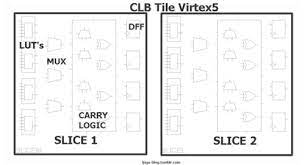
\includegraphics[width= 0.4\textwidth]{figure_1.1}\\
\caption{Structure of a Xilinx Virtex-5 Configurable Logic Block (CLB)}
\label{fig:figure_1.1}
\end{figure}

FPGAs are available either as standalone chips suitable for integration onto printed circuit boards (PCBs) or as part of integrated solutions where the FPGA is embedded within a specialized board. These integrated solutions typically come equipped with a module responsible for the FPGA programming and offer a range of standard interfaces including serial ports (UART), and Ethernet, as well as interfaces for external memory and storage devices.

\pagebreak
The primary advantages of FPGAs over traditional implementations include:
\begin{outline}
\1 FPGAs occupy a strategic middle ground between software-based solutions and Application-Specific Integrated Circuits (ASICs), offering faster implementations compared to software-based approaches, while remaining more cost-effective than ASICs.

\1 FPGAs liberate designers from reliance on component manufacturing and distribution chains, as the behavior of the device is not inherent to its physical structure but is determined by the designer's configuration.

\1 The reprogrammable nature of FPGAs fosters reusability and facilitates upgradability, enabling iterative refinement of designs without necessitating hardware replacements.

\end{outline}

\section{Communication Networks}
A computer network is defined as a set of interconnected devices purposed for facilitating communication among them.  Different types of networks exist, depending on their intended functions and operational constraints. The Internet is the largest network of interconnected computing devices.

Various technologies are available to choose from when connecting devices, including Ethernet cables, optical fibers, and wireless mediums leveraging electromagnetic waves such as microwaves. The selection of a particular technology depends on several criteria, with the most important considerations being performance and cost-effectiveness.

In addition to establishing physical interconnectivity among systems, the formulation of precise rules and communication protocols is required for any communication attempts to be successful. These communication protocols serve as the foundational framework underpinning the proliferation and diversification of network-centric applications.

Another important characteristic of networks is the transmission of information in the form of packets. Each packet encapsulates either the entirety or a portion of the transmitted data. Alongside the information intended to be transmitted (payload), packets include one or more headers containing information needed for the transmission of the packet itself. Intermediate network nodes leverage this header information to facilitate packet routing, whereas the payload content is exclusively intended for consumption by the ultimate recipient.


\subsection{Protocol Stack}
% Networks are based on the principle of modularity, meaning their entire operation is divided into individual and, as much as possible, independent functions. This approach allows us to address the complexity of these systems and, furthermore, makes them more flexible, as any necessary changes can be made without needing to rework the entire implementation, but only the relevant part.

Networks are structured upon the foundational principle of modularity, wherein their operational framework is compartmentalized into discrete and ideally autonomous functions. This modular approach not only reduces the inherent complexity of these systems but also enables flexibility and adaptability since modifications don't require a comprehensive overhaul of the entire architecture but rather focus on relevant segments.

% The protocol stack is a series of layers or levels of information processing for transmission/reception. This processing aims at the successful transmission/reception of information from one system (host) to another, and for successful communication, the stack must be implemented at each end of the communication. Each layer undertakes a specific function and provides services to the immediately higher layer of the stack. When information is sent, processing begins from the highest level to the lowest, with the final function being the transmission of data, while during reception, the reverse path is followed until the information is received.

Central to network operation is the protocol stack, comprising a hierarchical arrangement of layers dedicated to information processing of the transmitted information. This processing aims to ensure a seamless exchange of information between systems (hosts). This requires the existence of an implementation of the protocol stack at each end of the communication. Each layer within the stack assumes a distinct function and provides services to the layer above. During the transmission phase, information processing commences from the highest layer and cascades downward, reaching the lower layer where the physical transmission takes place, whereas, in the reception phase, the reverse path is followed, with the upper layer providing the information to the host application.

\begin{figure}
\centering
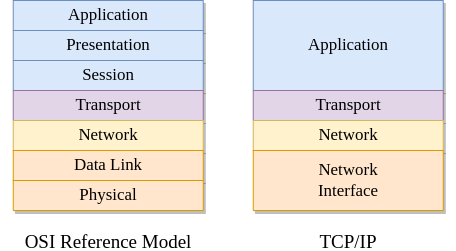
\includegraphics[width= 0.5\textwidth]{figure_1.2}\\
\caption{(left) The OSI stack, (right) the TCP/IP stack}
\label{fig:figure1.2}
\end{figure}

% The structure of the protocol stack has been standardized by the OSI (Open Systems Interconnection) model. The OSI model is based on a proposal developed by the International Standards Organization (ISO) as a first step towards the international standardization of protocols used in various network layers. It abstractly defines the layers, their functions, and their interconnections. It does not specify the protocols used at each layer but simply describes the functions that should be performed at each layer. Thus, there are many different protocols for each layer, each used for different purposes and covering different needs. These layers and their basic functions are:

The protocol stack's architecture is standardized by the OSI (Open Systems Interconnection) model, originating from a proposal developed by the International Standards Organization (ISO) to initiate global standardization of network protocols across diverse layers. The OSI model abstractly delineates these layers, their functionalities, and their interconnections. It refrains from specifying protocols but instead outlines the functions at each layer should perform. Consequently, a multitude of protocols exists for each layer, tailored to distinct purposes and addressing diverse requirements. The OSI layers are outlined as follows:

\begin{outline}
\1 Physical Layer\\
Responsible for data transmission across the physical communication channel, the Physical Layer is tasked with encoding/decoding data into the channel's respective code, such as electrical pulses (e.g., 0-5V for cable transmission) or optical pulses (for optical fiber transmission). Its primary objective is to ensure accurate reception of transmitted bits without degradation or misinterpretation.

\1 Data Link Layer\\
Assuming control over data transmission from the Physical Layer, the Data Link Layer ensures reliable data delivery, encompassing error detection, correction, and recovery procedures. It segments data into discrete frames for transmission and conducts error checking upon reception of each frame. Additionally, it may include traffic regulation mechanisms to regulate data flow and prevent congestion.

\1 Network Layer\\
It orchestrates the routing of information through intermediate systems to facilitate communication between non-directly connected systems and hosts belonging to disparate local networks.

\1 Transport Layer\\
Catering to scenarios where multiple applications or users seek access to the network, the Transport Layer manages the multiplexing and demultiplexing of data, ensuring accurate delivery to the intended recipient(s).

\1 Session Layer\\
Enabling users from different systems to establish sessions, the Session Layer offers services such as dialogue control, token management, and synchronization.

\1 Presentation Layer\\
In contrast to lower layers that focus on bit transmission, the Presentation Layer concerns itself with the syntax and semantics of transmitted information. It manages abstract data structures to facilitate interoperability among systems employing different data representations, facilitating standardized encoding for data exchange

\1 Application Layer\\
Comprising a suite of protocols catering to diverse user requirements, the Application Layer facilitates functions such as file transfer, email communication, and web page presentation. This is the layer where data is created and where transmitted data gets received.
\end{outline}\\


The Internet utilizes the TCP/IP stack, incorporating the TCP (Transmission Control Protocol) and IP (Internet Protocol) as its primary protocols. While adhering to the OSI model, the TCP/IP stack merges the transport and session layers within the application layer. Additionally, the lower layers (physical and data link) are often merged as well, forming a cohesive network interface layer. Figure ~\ref{fig:figure1.2} illustrates the OSI and TCP/IP stacks, highlighting their similarities and differences.

\begin{figure}[h!]
\centering
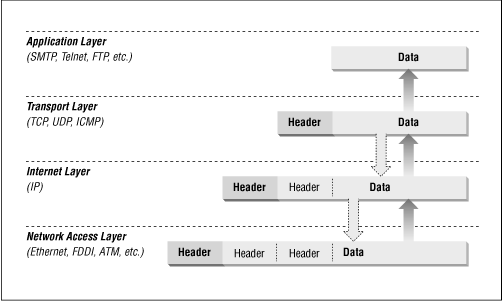
\includegraphics[width= 0.7\textwidth]{figure_1.3}\\
\caption{Packet transformation through the protocol stack}
\label{fig:figure1.3}
\end{figure}


During transmission, data originates at the application layer and traverses sequentially through the protocol stack until it reaches the physical layer for transmission. At each layer, the data received from the layer above is augmented with a suitable header, and in some cases, additional data may be appended to the "tail" of the packet. This iterative process, known as encapsulation, ensures that each layer includes information needed by its corresponding layer on the other side of the communication. During reception, the data first reaches the physical layer and moves upwards in the stack. Each layer successively processes and strips away its corresponding header, thereby progressively unveiling the core content of the packet. The core content is ultimately delivered to the application layer without any headers. The abstract representation of the packet format at each layer is depicted in Figure ~\ref{fig:figure1.3}.

\subsection{Network Security}
% The field of network security deals with the secure communication between networked systems, controlling access to network services and resources, as well as protecting and ensuring the proper functioning of individual systems and the network as a whole. It belongs to the domain of information security and applies basic concepts such as confidentiality and authentication in the realm of networks.

% A fundamental aspect of network security is the design, analysis, and implementation of security protocols. Beginning with the design phase, the objectives and services that the protocol will provide are initially defined. Subsequently, the protocol details are specified, including packet header formats, request-response mechanisms, algorithm usage, and other protocols. Additionally, during the design phase, scenarios under which the protocol will operate are defined and examined.

% Next, we proceed to the analysis phase, where the extent to which the design meets the objectives is evaluated, potential errors or omissions are identified, etc. Analysis may reveal the need for changes or expansions to the protocol design, prompting a redesign. This feedback loop continues until satisfactory results are achieved.

% Following the analysis, comes the implementation of the protocol, which involves considerations of performance, selection of implementation methods (hardware or software, programming language, etc.), and verification. At this stage, particular attention must be paid to the secure implementation of the protocol. Secure implementation does not solely concern the security of the protocol itself but also involves avoiding technical errors that may create security vulnerabilities. Thus, a protocol may offer a significant degree of security, but its implementation may render the system vulnerable to other types of attacks beyond those it was designed to protect against. Secure programming, secure hardware implementation, as well as physical placement and access methods of the system, are all aspects of secure implementation.

% Cryptology plays a significant role in network security as it provides the fundamental tools and mechanisms. Therefore, the security of networks, and information security in general, depends on the security of the cryptographic algorithms used and whether they are employed correctly.

% Common objectives in network security include the confidentiality and integrity of data, certification, availability of resources and services, as well as prevention methods and scenarios for recovering from attacks or malfunctions, concepts that will be elaborated upon in a subsequent chapter.

The domain of network security encompasses the establishment of secure communication channels among networked systems, the regulation of access to network services and resources, and the safeguarding of individual systems and the network as a cohesive entity. As part of the broader context of information security, network security is grounded in fundamental concepts such as confidentiality and authentication, tailored specifically to the realm of network environments.

Central to network security is the design, analysis, and deployment of security protocols. In the design phase, the objectives and services the protocol needs to provide are defined. Subsequently, the protocol details are specified, including packet header formats, request-response mechanisms, and algorithm choices. Furthermore, during the design phase, different operational scenarios are delineated and scrutinized.

In the analysis phase, the efficacy of the design in meeting predefined objectives is rigorously assessed, while potential flaws or oversights are identified and mitigated. The analysis is an iterative refinement process of revisions and enhancements until the protocol design satisfies its objectives.

Following analysis, the protocol is implemented. In this stage implementation and verification methodologies are selected. Of paramount importance is the secure implementation of the protocol. 
Secure implementation involves addressing technical flaws that could unintentionally create security weaknesses. Even if a protocol provides strong security features, an improperly implemented version could expose the system to unforeseen risks. Secure programming practices, secure hardware design, and defining access control are part of the secure implementation phase. The protocol implementation phase also includes performance and reliability considerations.

Cryptography assumes a pivotal role in the realm of network security, providing foundational tools and mechanisms for safeguarding network communications. Network security, and by extension, information security as a whole, relies on the robustness and correct usage of cryptographic algorithms.

Notable objectives of network security include data confidentiality and integrity, attestation mechanisms, resource availability, and the formulation of contingency plans for incident response and recovery, concepts that will be elaborated upon in subsequent chapters.
\clearemptydoublepage

% Chapter 2
\chapter{Cryptography and Security Protocols}\label{ch:chap2}
%!TEX root = ../main.tex

\section{Introduction}
Cryptography is the scientific field concerned with the study, development, and utilization of techniques aimed at secure communication between parties amidst the presence of adversarial entities seeking to intercept or manipulate transmitted data. In practice, it includes the creation and analysis of algorithms and protocols that aim to provide data confidentiality, data integrity, authentication, and non-repudiation. Modern cryptography is closely related to the fields of mathematics, computer science, and electrical engineering. Key concepts in this field include:
\begin{outline}
\1 Confidentiality, which ensures that only selected entities can access a set of information.

\1 Authentication, is the mechanism ensuring the genuineness of an entity's identity.

\1 Data Integrity, which verifies that data remains unaltered during transmission and detects any unauthorized modifications.
\end{outline}

A communication protocol is a definition of message formats and rules that are considered valid in communication. A protocol defines the syntax, semantics, and synchronization aspects of this communication. It stipulates the behavior of individual systems in an implementation-independent manner, allowing for protocols to be implemented in either hardware or software. For any successful communication, all participants must agree in advance on the protocols to be used.

A security protocol or cryptographic protocol protects communication using cryptographic methods. The fundamental services typically provided by cryptographic protocols are the authentication of participants, data integrity, and confidentiality, non-repudiation, and system availability (resilience to denial-of-service attacks). Alongside protocols directly protecting data, there exist protocols facilitating key exchange, negotiating communication parameters, and other auxiliary functions needed for establishing and maintaining secure communication.

Examples of cryptographic protocols include Transport Layer Security (TLS) which is used to secure HTTP traffic, the Diffie-Hellman key exchange which establishes a common secret over an insecure communication channel between two systems, and IPsec, which provides communication protection at the network layer of the TCP/IP stack.


\section{Cryptographic Algorithms}
Cryptographic algorithms serve as foundational elements in cryptography, offering essential mechanisms for secure systems. Due to their core position and heavy utilization in communication systems, attention to their efficiency is paramount.

There are various types of cryptographic algorithms, such as algorithms that provide data encryption, hashing, plausible deniability or deniable encryption, and steganography. Below we elaborate on the classes of cryptographic algorithms that are relevant to this thesis.


\subsection{Symmetric Cryptography}

Encryption is a transformation of a set of data into another, to secure this data from third-party access, i.e., aiming to provide confidentiality. The original data are called plaintext, while the data resulting from encryption are called ciphertext. The reverse transformation is called decryption.

Modern cryptography uses cryptographic keys for encryption and decryption, which parameterize the encryption algorithm. This parameterization decouples data confidentiality from cryptographic algorithm design. Assuming the algorithm is secure and implemented securely, then data confidentiality relies only on the secure protection of the key(s).

There are two basic types of encryption: symmetric and public key encryption. In symmetric encryption, a key is used for both encryption and decryption. The sender encrypts using the key, which is securely provided to the intended recipients, who in turn use it for decryption. Figure \ref{fig:figure2.1} illustrates the model of symmetric encryption.

% Figure 2.1
\begin{figure}[h!]
\centering
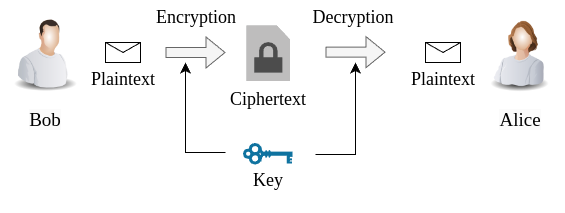
\includegraphics[width= 0.7\textwidth]{figure_2.1}\\
\caption{Symmetric Encryption}
\label{fig:figure2.1}
\end{figure}

% In symmetric encryption, two categories of algorithms prevail: block ciphers and stream ciphers. Block algorithms encrypt messages into equal-sized blocks, while stream algorithms encrypt bit by bit or byte by byte. The former are suitable when all data are available beforehand, whereas the latter encrypt data as it's generated (on-the-fly).

% For block algorithms, operation modes are crucial, detailing how the algorithm iterates over input data larger than the block size. When the input isn't a multiple of the block size, padding is employed to reach the appropriate size. The extended text is then inputted into the algorithm. Padding methods are typically specified in the algorithm's documentation. Various operation modes for block algorithms exist, including ECB, CBC, and CFB. Figure 2.2 illustrates CBC (Cipher-block Chaining).

Two categories of symmetric encryption algorithms exist, block ciphers and stream ciphers. Block ciphers encrypt a message into equal-sized blocks, while stream ciphers encrypt it bit by bit or byte by byte. The former are suitable when all data are available beforehand, whereas the latter encrypt data as it's generated (on-the-fly).

Block algorithms operate in modes that describe how the algorithm iterates over input data larger than the block size. When the input isn't a multiple of the block size, padding is employed to reach the appropriate size. The extended text is then inputted into the algorithm. Padding methods are typically specified in the algorithm's documentation. Various operation modes for block algorithms exist, including ECB, CBC, and CFB. Figure ~\ref{fig:figure2.2} illustrates the CBC (Cipher-block Chaining) mode \cite{rfc3602}.

% Figure 2.2
\begin{figure}[h!]
\centering
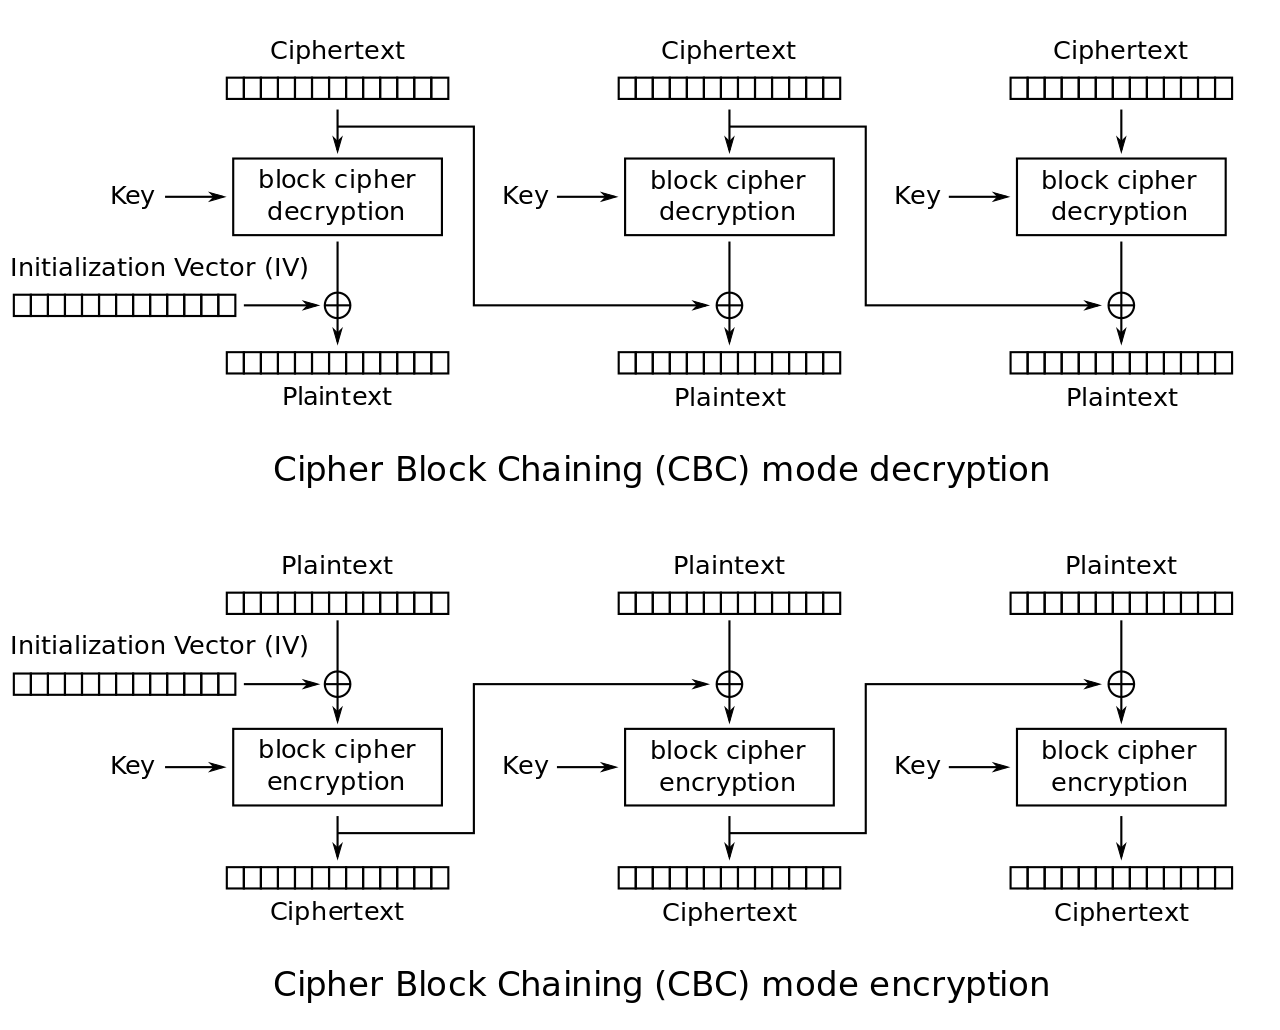
\includegraphics[width= 0.7\textwidth]{figure_2.2}\\
\caption{CBC Mode}
\label{fig:figure2.2}
\end{figure}

\newpage
\subsection{Public-Key Cryptography}
In public-key cryptography, each entity employs two keys: a public key and a private key. The public key is openly accessible, whereas the private key must be kept secret. These keys have the property that data encrypted with one key can be decrypted with the other. Furthermore, given the public key, discovering the private key is practically infeasible. Public-key algorithms serve two primary purposes: confidentiality and authentication.

When an entity wants to send information confidentially to another, it uses the other's public key to encrypt the data. Only the holder of the corresponding private key can access the plaintext. The process is illustrated in Figure ~\ref{fig:figure2.3}.

% fig 2.3
\begin{figure}[h!]
\centering
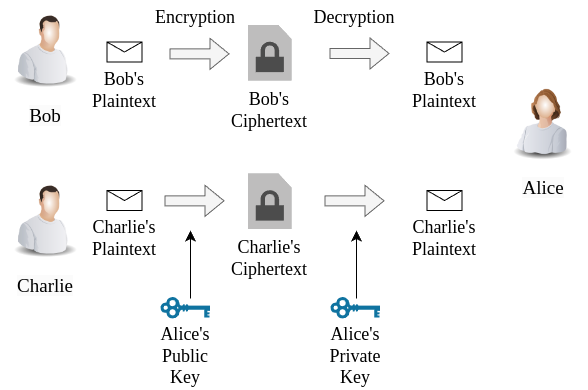
\includegraphics[width= 0.6\textwidth]{figure_2.3}\\
\caption{Public Key Encryption}
\label{fig:figure2.3}
\end{figure}

For authentication, the sender applies their private key to the data, generating a signature that is ideally impossible to forge.  Upon receipt, the recipient verifies the signature using the sender's public key. This process is illustrated in Figure ~\ref{fig:figure2.4}.


% fig 2.4
\begin{figure}
\centering
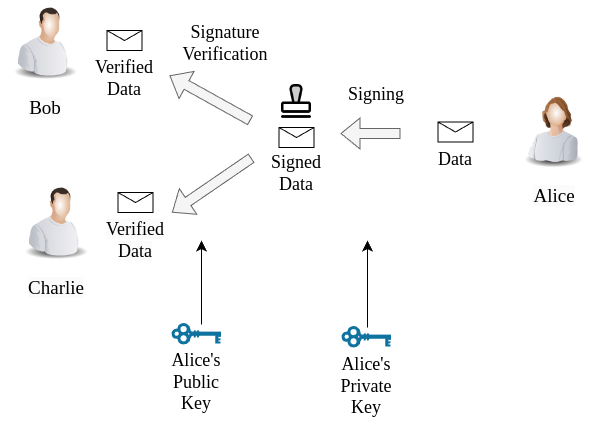
\includegraphics[width= 0.7\textwidth]{figure_2.4}\\
\caption{Public Key Signing}
\label{fig:figure2.4}
\end{figure}

Examples of applications of public key algorithms are digital certificates and secure key exchange (e.g., Diffie-Hellman) in TLS.



\subsection{Hash Functions}
A hash algorithm is a deterministic algorithm that maps variable-sized data to fixed-sized data, called hash or digest. Due to the finite number of potential outputs compared to the infinite input space, hash algorithms inevitably encounter collisions, where distinct inputs yield identical outputs.


% fig 2.5
% \begin{figure}
% \centering
% \includegraphics[width= 0.7\textwidth]{figure_2.5}\\
% \caption{}
% \label{fig:figure2.5}
% \end{figure}

In cryptographic applications, cryptographic hash functions adhere to additional stringent criteria:
\begin{outline}
\1 Difficulty in finding an input that generates a specific output.
\1 Difficulty in modifying the input while keeping the output the same.
\1 Difficulty in discovering two inputs that produce identical outputs.
\end{outline}

The higher the degree of the above difficulties, the greater the hash algorithm's security. Cryptographic hash algorithms primarily serve serve data authentication and integrity purposes. Notable examples include MD5, RIPEMD, and SHA \cite{fips_118_2}.


\subsection{Keyed Hash Functions}
To ensure data integrity and authentication, message authentication codes (MACs) are commonly employed. A MAC consists of a small piece of information appended to the message to enable verification upon receipt. Cryptographic hash algorithms are often used in conjunction with a key (Hash-based MAC – HMAC) which is accessible solely to the communicating endpoints. Any cryptographic hash algorithm, such as SHA-1 and MD5, can compute an HMAC, resulting in algorithms like HMAC-MD5 and HMAC-SHA-1, respectively. The process is depicted in Figure \ref{fig:figure2.6}.

% fig 2.6
\begin{figure}
\centering
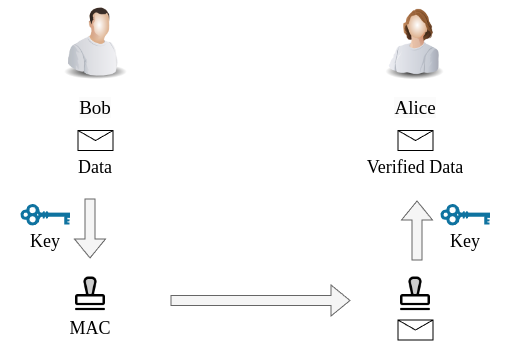
\includegraphics[width= 0.6\textwidth]{figure_2.6}\\
\caption{HMAC Operation}
\label{fig:figure2.6}
\end{figure}

\subsection{Pseudorandom Number Generators}
Random Number Generators (RNGs) are algorithms designed to generate sequences of numbers that mimic randomness. Two categories of RNGs are True RNGs and Pseudo RNGs.  True RNGs are generators that usually generate numbers from random physical phenomena while Pseudo RNGs usually rely on a small amount of physical randomness, called seed, which they use to further generate numbers that appear random but are not truly random as they still exhibit patterns and repetitions. 

In cryptography, RNGs play a vital role when randomness is required for security. They are commonly utilized in tasks such as cryptographic key generation and initialization vector creation.

\section{Key Management}
Key management encompasses key creation, distribution/exchange, storage, and replacement—a crucial process for system security often challenging to implement due to policy considerations and external factors.

Before initiating secure communication, entities must establish communication parameters, including cryptographic keys for symmetric encryption. Key exchange facilicates the need to establish such keys over insecure communication channels. A notable key exchange protocol is the Diffie-Hellman exchange.

Keys undergo a lifecycle, necessitating periodic replacement. This practice mitigates risks associated with key compromise. Regular replacement limits the impact of key exposure and adds complexity for malicious entities, as it reduces the volume of data encrypted with a single key, thereby limiting available data for cryptanalysis.

\section{Security Hardening}
Several considerations are involved when trying to improve the security of a cryptographic system. One of the most important parameters in security is the key size. It directly correlates with security strength; larger sizes correspond to increased security levels. Furthermore, encryption algorithms are evaluated based on the important properties of confusion and diffusion. Cryptographic hash algorithms should exhibit collision resistance, making collisions difficult to find. Similarly, an effective pseudorandom number generator should produce sequences with extended periods before repetition. Beyond these algorithmic properties, additional techniques are employed to bolster security at the implementation level, such as side-channel countermeasures and formal verification techniques.


\subsection{Padding}
In addition to configuring appropriate input sizes for block algorithms, data extension also helps conceal the actual size of the data packet. Additional padding can be used as a way to increase security albeit at the cost of throughput.


\subsection{Salt}
The term "salt" is used to denote additional data added to the input of hash algorithms. Adding salt to the input results in a different output from the algorithm, even with the same input. This method mitigates attacks such as rainbow tables.


\subsection{Initialization Vectors}
An Initialization Vector (IV) is random data the size of a block which is placed at the beginning of the plaintext data, with the aim of further enhancing the security of block algorithms. They introduce randomness into the encryption process since for encrypting the same text under the same key, the result will depend on the IV value. The requirement for IVs is that they need to be unpredictable.







\clearemptydoublepage

% Chapter 3
\chapter{The IPsec Protocol Suite}\label{ch:chap3}
%!TEX root = ../main.tex

\section{Overview}\label{ch:3.1}
IPsec (Internet Protocol Security) comprises a suite of protocols designed to secure communications at the IP (Internet Protocol) level across both IPv4 and IPv6 \cite{rfc2460} versions. It provides authentication and/or encryption services for each IP packet within a communication session. Additionally, IPsec encompasses protocols for mutual authentication during session initiation and cryptographic key negotiation. Optional features include packet replay protection. Its specifications are outlined in various RFCs (Request for Comments), detailing protocol components and their interactions.

Operating at the Network layer of the TCP/IP stack \cite{rfc4301}, IPsec serves as an end-to-end security mechanism. It safeguards communication between hosts (Host-to-Host), between Security Gateways (Network-to-Network), or between an end and a Security Gateway (Network-to-Host).

% fig 3.1
\begin{figure}[h!]
\centering
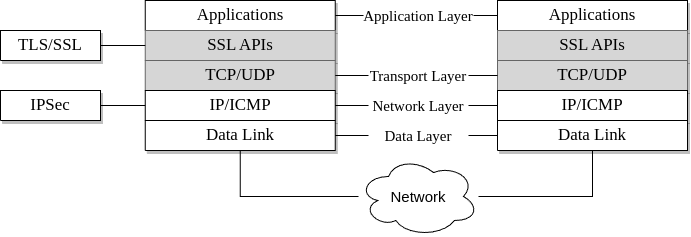
\includegraphics[width= 0.9\textwidth]{figure_3.1}\\
\caption{IPsec's position in the network stack}
\label{fig:figure3.1}
\end{figure}

Operating at the Network layer enables IPsec to provide its services independently of which protocols are utilized at higher layers, while ensuring protection across all layers above it and, optionally including the IP layer.

IPsec defines two protocols: the Authentication Header (AH) \cite{rfc4302} and the Encapsulating Security Protocol (ESP) \cite{rfc4303}. AH offers data integrity, data origin authentication, and optional anti-replay protection, whereas ESP augments AH's functionalities by including data confidentiality \cite{rfc3602}. Utilized cryptographic algorithms include HMAC-SHA1 (\cite{rfc2104}, \cite{rfc4634}, \cite{rfc2404}) and HMAC-MD5 for integrity and authentication, along with AES \cite{fips197} and 3DES for confidentiality. Nevertheless, the framework accommodates the utilization of alternative cryptographic algorithms as needed.

In IPsec, two communication modes are defined: Transport mode and Tunnel mode. Transport mode secures end-to-end communication (Host-to-Host), whereas Tunnel mode extends protection to Network-to-Network and Network-to-Host scenarios. Figures \ref{fig:figure3.2}, \ref{fig:figure3.3}, and \ref{fig:figure3.4} visually depict these communication modes, with the green line denoting the secured segment of the route.

% fig 3.2
\begin{figure}[h!]
\centering
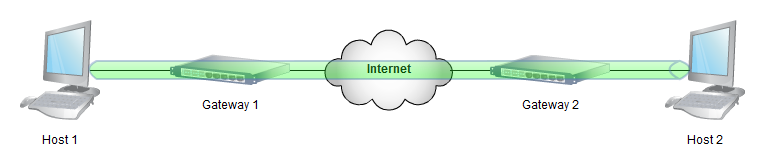
\includegraphics[width= 0.9\textwidth]{figure_3.2}\\
\caption{Host-to-Host in Transport Mode}
\label{fig:figure3.2}
\end{figure}

% fig 3.3
\begin{figure}[h!]
\centering
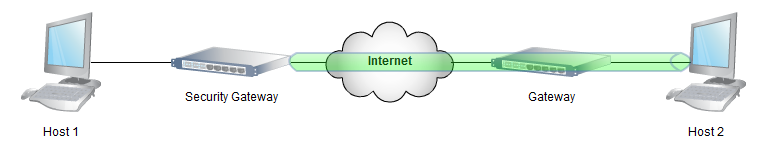
\includegraphics[width= 0.9\textwidth]{figure_3.3}\\
\caption{Network-to-Host in Tunnel Mode}
\label{fig:figure3.3}
\end{figure}


% fig 3.4
\begin{figure}[h!]
\centering
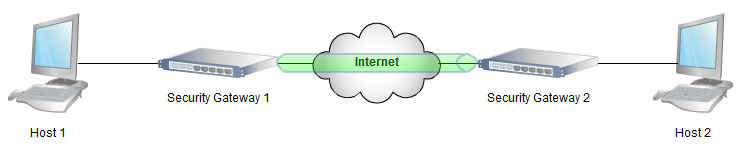
\includegraphics[width= 0.9\textwidth]{figure_3.4}\\
\caption{ Network-to-Network in Tunnel Mode}
\label{fig:figure3.4}
\end{figure}

% Before initiating a secure communication several parameters should be defined and agreed upon. These include the cryptographic algorithms to be used, the keys, the protocol to be applied (AH or ESP), etc. A collection of choices for these security parameters constitutes a Security Association (SA). For each new secure session, an SA should be created at both ends of the communication.

Before initiating secure communication, various parameters must be established and mutually agreed upon, including cryptographic algorithms, keys, and the chosen protocol (AH or ESP). A choice of these security parameters constitutes a Security Association (SA), For each new secure session, an SA should be created at both ends of the communication.

The establishment of SAs within IPsec can be manual or automated. Manual configuration necessitates users to specify parameters at both ends, potentially involving intermediate Security Gateways. Manual configuration has many drawbacks such as maintenance overheads and susceptibility to human errors, hence automated methods are generally favored. The Internet Key Exchange Protocol (IKE) orchestrates automated parameter negotiation, secure key exchange, and maintenance, drawing upon the Oakley and ISAKMP protocols.

Security associations contain the parameters for secure communication. However, they do not determine whether the two ends are legitimate to communicate via IPsec. This determination, as well as whether IPsec should be used in the communication, is defined through the Security Policy (SP) mechanism. Security policies are a management mechanism for IPsec users. Thus, system users define, at a higher level, the nature of communication with other systems, without being concerned with low-level details (algorithms, keys, etc.). The actions defined in IPsec policies are three: Protecting traffic (Apply IPsec, Protect), Bypassing IPsec, or Discarding traffic. Security policies have a set of selectors to filter traffic and determine which policy it belongs to.

While security associations define parameters for secure communication, they do not ascertain when IPsec needs to be used and between which entities. These parameters are controlled through the Security Policy (SP) mechanism. SPs serve as a management framework for IPsec users, allowing higher-level specification of the nature of communication with other systems without delving into low-level details such as algorithms and keys. SPs use 'selectors' to identify what policy to apply to which communication. SPs also define what actions need to be taken for a given communication. The options for SP actions are:
\begin{outline}
    \1 Protect (apply IPsec)
    \1 Bypass (send/process the packet without applying IPsec)
    \1 Discard (do not send/process the packet)
\end{outline}

When implementing IPsec, one has to consider how to integrate it with the rest of the protocol stack. Three options exist:
\begin{outline}
\1 Native:\\
IPsec is implemented within the protocol stack. Access to the stack code is required for integration.
\1 Bump-in-the-stack (BITS):\\
IPsec is implemented "below" a deployed version of the IP layer, between the network layer and the network interface. Access to the source code is not required for this choice. This approach is preferred when integrating IPsec in commercial closed-source products.
\1 Bump-in-the-Wire (BITW):\\
IPsec is implemented in an external device rather than within the systems that utilize it. This method is common in military and some commercial applications. The embedded device acts as an "assistant" to the host system and often has its own IP address.
\end{outline}

\subsection{Outbound Packet Processing}
IPsec defines the flow of outbound packet processing as follows:
\begin{outline}

\1 Initially, information in the header of the outgoing packet is used to identify a policy that can be applied to this traffic. If no matching policy is found, the packet is discarded (Discard action).

\1 If a policy is found, it is applied. If the action is to Bypass, no further action is required by IPsec, and the packet continues its usual path through the stack. If the action is Discard, the packet is dropped. If the action is Protect, the SA pointed by the policy is queried, and the specific security parameters in the SA are used. If no SA is found and if automated SA creation is supported then the key manager (e.g. IKE) gets invoked. If the key manager fails or there is no support for automated SA creation, the action defaults to Discard.

\1 Finally, if the packet has not been discarded, it is sent.
\end{outline}

The flowchart for the above process is presented in Figure \ref{fig:figure3.5}.

% fig 3.5
\begin{figure}
\centering
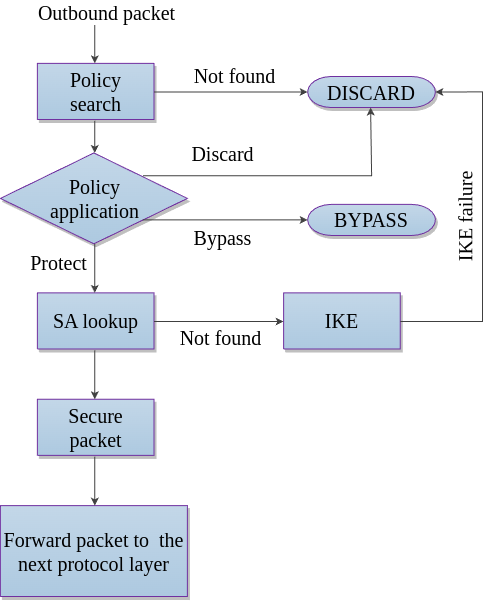
\includegraphics[width= 0.6\textwidth]{figure_3.5}\\
\caption{ Outbound packet processing flowchart}
\label{fig:figure3.5}
\end{figure}

\subsection{Inbound Packet Processing}

IPsec defines the flow of outbound packet processing as follows:
\begin{outline}

\1 Initially, information in the header of the outgoing packet is used to identify a policy that can be applied to this traffic. If no matching policy is found, the packet is discarded (Discard action).

\1 In the case where the policy action is Protect, the corresponding SA is searched using a Security Parameter Index (SPI) present in the incoming packet, and the security parameters in the SA are used. If no SA is found, the packet is discarded.

\1 After applying the SA, the processed packet is checked against its corresponding policy to verify its correct protection.
\end{outline}

The above process is presented in flowchart form in Figure \ref{fig:figure3.6}.

% fig 3.6
\begin{figure}
\centering
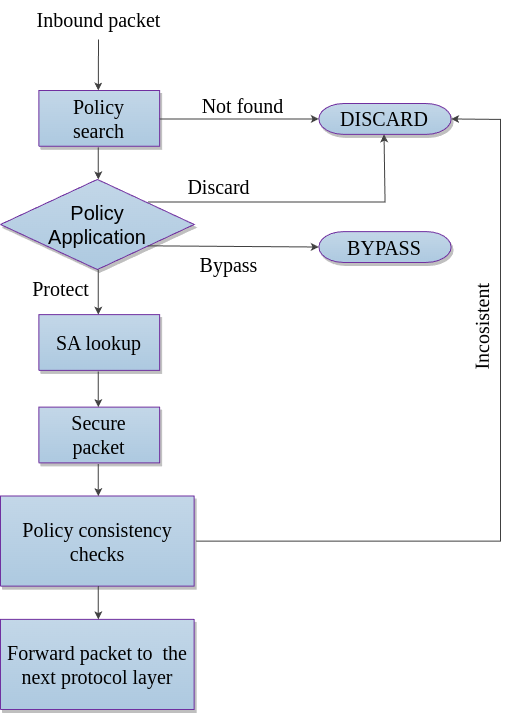
\includegraphics[width= 0.6\textwidth]{figure_3.6}\\
\caption{ Inbound packet processing flowchart}
\label{fig:figure3.6}
\end{figure}

\subsection{Transport and Tunnel Modes}
As previously stated, IPsec protocols can operate in either Transport mode or Tunnel mode. The difference in these two modes lies in which parts of the IP packet are considered the designated "payload" of the IPsec packet. In Transport mode,  only the data of the higher layer is considered as payload, while in Tunnel mode, the payload is extended to include the IP header. Figures \ref{fig:figure3.7} and \ref{fig:figure3.8} illustrate the packet format for Transport and Tunnel mode respectively, for both AH and ESP.

% fig 3.7
\begin{figure}[H]
\centering
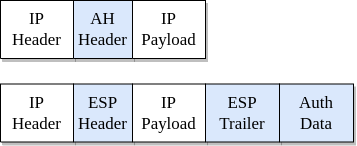
\includegraphics[width= 0.5\textwidth]{figure_3.7}\\
\caption{ AH (up) and ESP (down) packet formats in Transport Mode}
\label{fig:figure3.7}
\end{figure}

% fig 3.8
\begin{figure}[H]
\centering
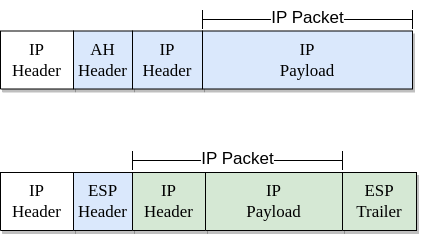
\includegraphics[width= 0.5\textwidth]{figure_3.8}\\
\caption{ AH (up) and ESP (down) packet formats in Tunnel Mode}
\label{fig:figure3.8}
\end{figure}


In transport mode, only the hosts execute IPsec. Initially, the appropriate protection is applied to the packet by the sender, and then the corresponding header is added to the data of the higher protocol. This is followed by the addition of the IP header, and finally, the packet is sent to the destination address. When it reaches the recipient, the packet is processed by IPsec, and the resulting payload is handed to the appropriate higher-layer protocol.

In tunnel mode, one or two Security Gateways (SGs) are involved. In the scenario of network-to-network tunnel mode, two SGs are used. The process starts with the packet being sent by the sender as normal. When the packet reaches the local SG, IPsec protection is applied to the entire IP packet. Then the security protocol header is added at the position right after the original IP header. Subsequently, a new IP header is added, containing the addresses of both the local and remote SGs, and finally packet is transmitted. When the packet reaches the remote SG, it is processed by IPsec, resulting in the original IP packet. Then, the IP packet is forwarded unmodified to the local network to reach its final recipient.

In the network-to-host scenario, where only a single SG is involved, two things change compared to the network-to-network scenario. Firstly, during transmission at the end of the communication where there is no SG, the host assumes SG's processing responsibilities. In other words, the host is effectively acting as its own SG. Secondly, during packet transmission from the SG-equipped end, the SG only routes the packet without applying tunnel mode processing. Thus, in network-to-host scenarios, tunnel mode operates from the host to the SG, transitioning to transport mode from the SG-equipped end to the host.


\section{Security Associations (SA)}
As previously mentioned, a Security Association (SA) is a data structure containing information regarding the parameters governing a security session. SAs encapsulate parameters for each unidirectional session, leading to the utilization of two SAs per node in bidirectional scenarios — one for inbound and one for outbound traffic. These SAs are stored in a database known as the Security Association Database (SADB). Each SA is uniquely identified by a Security Parameter Index (SPI) which is used during search and retrieval of SAs. Both AH and ESP packets have a dedicated field within their headers designated for storing the SPI value corresponding to the applicable SA. SAs can be defined either manually by the system user or automatically through a negotiation protocol. Moreover, they have a lifetime limit, meaning they are invalidated after a certain period, and a new negotiation must start. An SA entry includes:
\begin{outline}
\1 The security protocol used (AH or ESP)
\1 The mode used (Transport or Tunnel)
\1 A Sequence Number for Anti-Replay
\1 Information about the authentication algorithm used in AH, such as the algorithm type, the key id, etc.
\1 Information about the encryption algorithm used in ESP, such as the algorithm's mode, the key id, the initialization vector, etc.
\1 Information about the data integrity algorithm used in ESP
\end{outline}

\section{Security Policy Database (SPD)}
The defined Security Policies are stored in the Security Policy Database (SPD). SPD facilitates the search for the appropriate policy for a specific packet. The order in which policies are stored in the SPD also defines their priority of application. Each security policy is a data structure that holds information used for matching the policy to a specific type of traffic. The specific types of this information are called selectors and they include:
\begin{outline}
\1 lists of local IP addresses
\1 lists of remote IP addresses
\1 higher-layer protocol
\1 local port
\1 remote port
\end{outline}

An SP entry includes:

\begin{outline}
\1 The type of policy to be applied. The three possible values are Protect, Bypass, and Discard. In the case of Protect, additional information is included in the SP:
\2 the IPsec mode
\2 for Tunnel Mode, the local and remote IP addresses of the tunnel
\2 the security protocol to be applied
\2 a prioritized list of algorithms that are allowed to be used. This information is useful in determining which algorithm will be used during an SA negotiation
\2 the SPI of the SA that this policy can use
\end{outline}

\section{The Authentication Header (AH) Protocol}
The AH protocol provides authentication, data integrity, and optional anti-replay protection for IP packets. Protection is provided for most of the IP packet and higher-layer protocol data,  however, since some fields in the IP header can change during transit and thus their final values cannot be predicted, they are committed from AH protection.

AH defines a header format that provides information regarding the packet's protection. The format of the header is shown in Figure \ref{fig:figure3.9}. The fields' purposes are:

\begin{outline}
\1 Next Header: \\The 8-bit standardized number (IANA) of the protocol that AH encapsulates. In tunnel mode, it can take only take the values 4 for IPv4 or 41  for IPv6.
\1 Payload Length: \\An 8-bit field denoting the size of the entire AH packet, expressed as a multiple of 32 bits and reduced by 2.
\1 Reserved: \\Reserved for future use. Mandated to be set to 0 by the sender, with no recipient verification requirement.
\1 Security Parameter Index (SPI):\\ A 32-bit value pointing to the applicable SA.
\1 Sequence Number: \\An unsigned 32-bit integer denoting the packet's sequence number within the SA session. It is used by the anti-Replay mechanism. The field is mandatory, even when anti-replay is decativated.
\1 Authentication Data (or Integrity Check Value – ICV):\\ A variable-sized field containing the outcome of the integrity/authentication algorithm. This field must be an integer multiple of 32 bits. Padding is included for proper alignment of the packet on a 32-bit boundary.
\end{outline}

% fig 3.9
\begin{figure}[H]
\centering
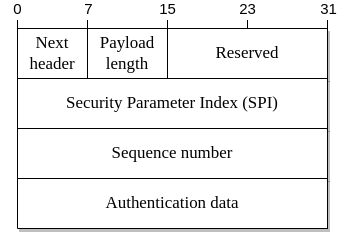
\includegraphics[width= 0.5\textwidth]{figure_3.9}\\
\caption{ Structure of the AH protocol header }
\label{fig:figure3.9}
\end{figure}

\subsection{Outbound Packet Processing}
The outbound packet processing for AH is as follows:
\begin{outline}[enumerate]
\1 Finding SA: \\The AH protocol is applied when the SA corresponding to this traffic designates it as the protocol.

\1 Sequence Number calculation:\\ The sender starts the Sequence Number counter at 0 and increments it by 1 for each subsequent outgoing packet. Its value is stored in the SA. In the case of automatic SA creation and if the counter has returned to 0 after traversing all values, the SA expires and a new one must be created. If SA management is manual, then the counter restarts from 0.

\1 ICV calculation: \\Calculation of the ICV involves the payload, the AH header, and a portion of the outer IP header. The value of the Authentication Data field is assumed to be all zeros for this calculation. From the IP header, only the fields that remain constant in the packet's path (immutable) are selected. The rest (mutable), their values are assumed as 0. The mutable fields of the IPv4 header are TOS, Flags, Fragment Offset, TTL, and Header Checksum. For IPv6, they are TOS, Flow Label, and Hop Limit. The calculated ICV value is placed in the Authentication Data field.

\1 Padding: \\Finally, if necessary, padding is applied to ICV so that the entire packet is a multiple of 32 bits in IPv4 and a multiple of 64 bits in IPv6. Additional padding may be required to make the packet size a multiple of the block size of the algorithm used for authentication/integrity.
\end{outline}

\subsection{Inbound Packet Processing}
The inbound packet processing for AH is as follows:
\begin{outline}[enumerate]
\1 Finding SA:\\ Firstly, SPI is used to locate an applicable SA. If no SA is found, the packet is discarded.

\1 Anti-replay:\\ If the anti-replay protection is enabled, the Sequence Number is checked. If found correct the processing continues; otherwise, the packet is discarded.

\1 ICV verification:\\ The receiver calculates the ICV in the same way as the sender. It then checks if the calculated value matches the value contained in the packet. If they do not match, then some alteration has occurred during the packet's transmission, and the packet is discarded.
\end{outline}

\section{The Encapsulation Security Payload (ESP) Protocol}
The ESP protocol provides authentication, data integrity, confidentiality, and optionally anti-replay protection. The set of services it provides is determined by the corresponding SA. Authentication and integrity are always provided together, which makes three combinations of services possible:
\begin{outline}
\1 Confidentiality only
\1 Authentication-integrity only
\1 Confidentiality and authentication-integrity
\end{outline}

ESP uses both a header and a trailer for the packet. The format of an ESP packet is shown in Figure \ref{fig:figure3.10}. The fields' purposes are:
\begin{outline}
\1 SPI: \\As with AH, this is the index for the corresponding SA.
\1 Sequence Number:\\ As with AH, this is the incrementing number for the anti-replay protection.
\1 IV (Initialization Vector):\\ This is an optional field. It is used when an IV is required by the encryption algorithm.
\1 Padding: \\ This field has two purposes. If a block encryption algorithm is used, it aligns the packet to the block size. Otherwise, it aligns the packet to a multiple of 32 bits. The contents of the padding bytes are determined either by the encryption algorithm or the default padding is used. This default padding is the monotonically increasing integer sequence starting from 1.
\1 Pad Length: \\ This field holds the length of the padding field in, expressed in bytes.
\1 Next Header: \\ The IANA number of the higher-layer protocol.
\1 Authentication Data: \\ A variable size field containing the result of the authentication/integrity algorithm. The size of this field is determined by the specific algorithm.
\end{outline}

% fig 3.10
\begin{figure}
\centering
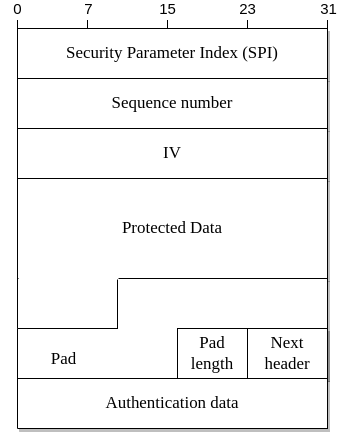
\includegraphics[width= 0.5\textwidth]{figure_3.10}\\
\caption{ Structure of the ESP protocol header }
\label{fig:figure3.10}
\end{figure}

\subsection{Outbound Packet Processing}

During outbound packet processing, once the SA corresponding to the outgoing packet is found and if the SA specifies the use of the ESP protocol, the following actions are taken:

\begin{outline}[enumerate]
\1 Padding is initially applied to the payload, so that the packet size becomes a multiple of 32 or 64 bits (for IPv4 and IPv6 respectively), or so that it becomes a multiple of the block size of the encryption algorithm. Additionally, the Payload Length and Next Header fields are inserted.

\1 Next, if confidentiality is required, the encryption algorithm is executed on the payload. The corresponding key, and, if required, IV, are provided by the SA.

\1 If an IV is required, it is placed at the start of the payload, following the ESP header.

\1 The Sequence Number is then calculated and the ESP header is inserted.

\1 Finally, if an authentication/integrity is required, the ICV is computed over the header and payload of the packet, and the result is placed in the trailer's Authentication Data field. The key and any other data needed by the algorithm are provided by the SA.
\end{outline}

\subsection{Inbound Packet Processing}
To begin processing an incoming packet with ESP, the corresponding SA must first be found and must specify that ESP processing needs to take place. If no SA is found, the packet is discarded. Otherwise, the following steps are taken:
\begin{outline}[enumerate]
\1 Initially, if anti-replay protection is used, the Sequence Number value is checked. If found correct, the packet processing continues. Otherwise, the packet is rejected.

\1 If authentication/integrity is used, the ICV of the packet is computed and compared with the ICV value in the packet. The key is provided by the SA. If the ICV values match, the packet passes the authentication/integrity check; otherwise, it is rejected.

\1 Next, if confidentiality is used, the decryption algorithm is executed using the key provided by the SA and, if available, the IV contained in the packet.

\1 Finally, the padding is removed and the result is the plaintext payload.
\end{outline}

\section{Key Management}
In IPsec, key management is performed using the Internet Key Exchange (IKE) protocol. IKE is a complex protocol based on the Oakley and ISAKMP protocols. Its purpose is the automated creation and management of Security Associations (SAs). Its main responsibilities include:

\begin{outline}
\1 Creating new SAs: This is achieved through a series of negotiations between the two communication ends regarding communication parameters such as authentication and encryption algorithms, keys, etc.
\1 Monitoring SA expiration and renegotiating them.
\end{outline}

IKE is executed in two phases. First, ISAKMP is used to generate an ISAKMP Security Association which establishes a secure communication channel. Then, this secure channel is used to negotiate IPsec SAs, in pairs. The first phase has various execution modes, namely Main Mode, Aggressive Mode, and Base Mode. Each mode is defined as a series of messages consisting of various headers and payloads. The second phase has only one mode, Quick Mode. Additionally, there are other message exchanges for various IKE functions that are not part of these two phases, such as New Groups Mode, Unacknowledged Notification exchanges, and Acknowledged Notification exchanges.

Before IKE executes, the identities of the two ends must be authenticated. IKE uses three methods for authentication: a pre-shared secret key, digital signatures, or public key encryption.

\clearemptydoublepage

% Chapter 4
\chapter{System Overview}\label{ch:chap4}
%!TEX root = ../main.tex

\section{Design Goals}
The present thesis produced an implementation of IPsec utilizing a hardware and software co-design approach. The target of the implementation is the FPGA board Virtex-5 ML505-ML509 Revision A \cite{ml505_user_guide}, housing the Virtex-5 XC5VFX70T FPGA. For software execution, the Microblaze soft-core processor \cite{mb_user_guide} is employed. Additionally, the system requires an Ethernet interface which is provided on the board along with the necessary drivers from Xilinx. Finally, an external DDR2 SDRAM memory is used for storing and executing the software. It should be noted that the system can be implemented using any board and processor, as long as an Ethernet interface, sufficient FPGA area, and enough memory for software execution are provided.

The library lwIP, an open-source implementation of the TCP/IP stack for embedded systems, is used. A port of lwIP to the specific FPGA board is provided by Xilinx. Additional modifications were made in the course of this thesis to incorporate IPsec.

For programming and debugging the system, a PC with an installation of Xilinx's ISE suite is used. Programming of the board is performed through a JTAG-to-USB cable, and debugging is performed through the board's serial port using a UART-to-USB cable.

Furthermore, a computer with the Linux operating system is used, where the IPsec Linux implementation "ipsec-tools" is installed. This computer is connected via Ethernet to the FPGA board, and both systems are configured to communicate using IPsec. This setup allows monitoring of incoming and outgoing packets. It also allows the verification of the system against a mainstream IPsec implementation.


\section{Design Decisions}

The system is implemented as an embedded system on an FPGA. This implementation environment has various constraints as well as advantages. Some of the constraints considerations include the available hardware area, the available peripherals, and the speed of the Microblaze soft-core processor. The main advantage includes the rapid development, implementation, and testing of hardware components.

Taking the above into consideration, various design choices are made aiming for the best possible utilization of the implementation environment's properties. These choices are explained in the following subsections.


\subsection{Native Implementation}

As mentioned in Chapter ~\ref{ch:3.1}, there are three ways the integration of IPsec can be performed. The chosen approach for this implementation is the "Native" approach. This is because the software package lwIP (lightweight IP), is readily available for our target hardware. Additionally, this package is open-source, giving us the option to directly modify its source code.

While a ready implementation of the TCP/IP stack, removes the additional effort of implementing the necessary protocols for the system to function as a network system, it requires an in-depth study of the lwIP code and specification in order to leverage its capabilities and establish proper interfacing between the two systems (lwIP and IPsec).


\subsection{Hardware and Software}\label{ch:4.2.2}

The available development environment enables the implementation of both hardware and software components. Certain modules can be selected for hardware implementation, while others can be executed in software. These subsystems can collaborate (hardware-software co-design), leveraging the benefits of each and mitigating their drawbacks.

In this thesis, the essential components of IPsec are implemented. Both AH and ESP protocols are integrated, covering both transport and tunnel modes. Additionally, both SADB and SPD are incorporated. The system can function as both a host and an SG. AH and ESP header processing, as well as the management of SPD and SADB databases, are implemented in software as part of the modified lwIP. The decision to develop these components in software is driven by the advantages of expedited development and debugging, facilitating better integration of IPsec with lwIP.

The cryptographic algorithms CBC-AES-128 and HMAC-SHA-1-96 are implemented in hardware. This decision is motivated by their role as latency and throughput bottlenecks, which are significantly alleviated by the faster speeds and parallel processing offered by hardware implementations.

Manual SA management is the only supported method. This choice is made due to the complexity and size of the IKE protocol, which is deemed beyond the scope of this thesis.

Additional features of the system include support for anti-replay protection and a generalized interface to cryptographic algorithms, simplifying the integration of different algorithms.
\clearemptydoublepage

% Chapter 5
\chapter{Hardware Components}\label{ch:chap5}
%!TEX root = ../main.tex

\section{Architecture}
The system consists of a Microblaze processor, a DDR2 SDRAM memory, peripheral systems for Ethernet and UART interfacing, as well as units for cryptographic algorithms. All subsystems are connected to the processor via a PLB (Processor Local Bus) bus. Additional peripherals required during design include an interrupt controller and a timer. The interrupt controller manages interrupts from coming from the Ethernet, UART, and the timer. The timer is required by lwIP for time measurements. The architecture of the system is depicted in Figure \ref{fig:figure_5.1}.

% fig 5.1
\begin{figure}[H]
\centering
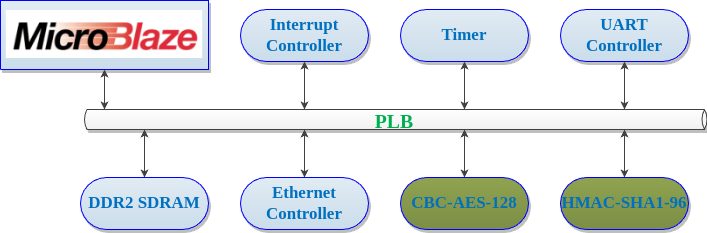
\includegraphics[width= 0.8\textwidth]{figure_5.1}\\
\caption{ High-level system architecture }
\label{fig:figure_5.1}
\end{figure}

Each peripheral system is assigned its own address range when integrated with Microblaze (Address Mapped IO). The transfer of data to and from the memory of the cryptographic peripheral systems is handled by Microblaze (i.e., there is no Direct Memory Access - DMA system). This is because the system does not operate in multipacket mode which means that it is not capable of processing more than one packet simultaneously. This is because lwIP does not utilize threading when deployed in bare-metal, but instead relies on an operating system (e.g., Linux or XilKernel).

\section{Custom Cryptographic IP Cores}
\subsection{CBC-AES-128}
\subsubsection*{Algorithm Specification}
The CBC-AES-128 consists of the block symmetric encryption algorithm AES-128 in CBC mode (see Figure \ref{fig:figure2.2}). The number '128' indicates the size of the key in bits (the algorithms AES-196 and AES-256 are defined correspondingly). It gets a 128-bit block as input and outputs the encrypted block.

Internally, the algorithm consists of two operations: the encryption/decryption dataflow and the internal key generation dataflow. The encryption/decryption dataflow executes 10 iterations (rounds) of the basic encryption/decryption procedure when the key size is 128 bits (12 rounds for 196 bits and 14 rounds for 256 bits). Similarly, the internal key generation involves a 10-round process.
% fig 5.2
\begin{figure}
\centering
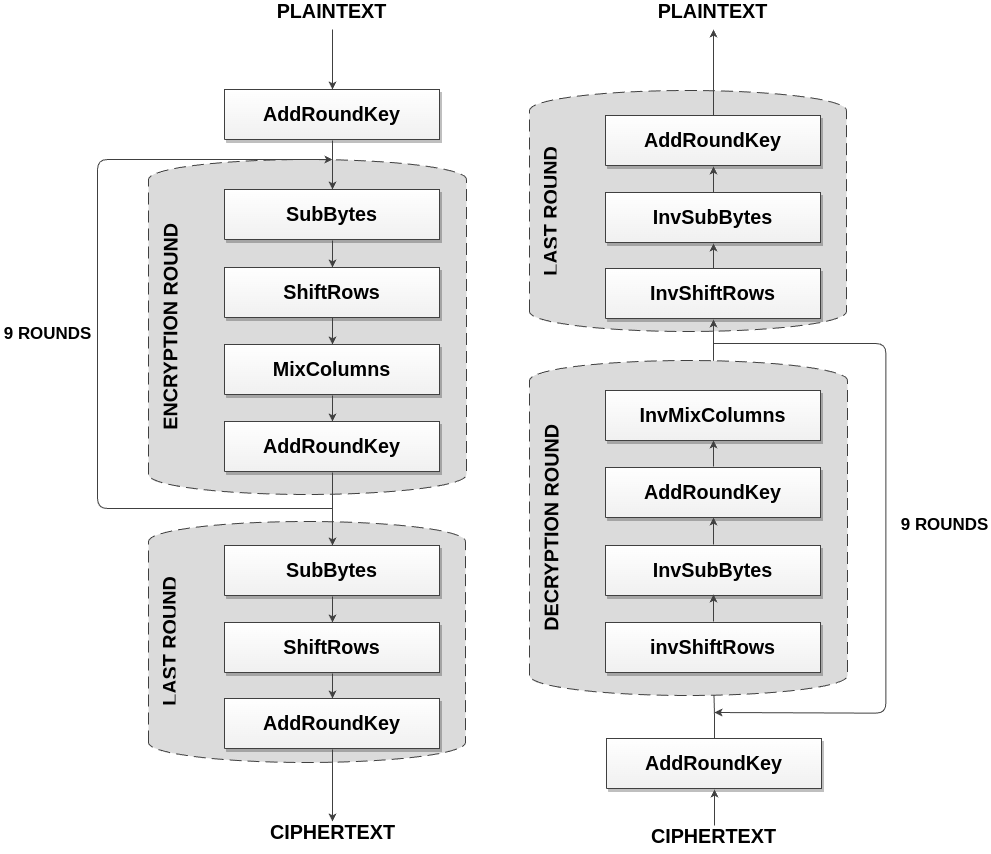
\includegraphics[width= 0.8\textwidth]{figure_5.2}\\
\caption{ (left) AES encryption algorithm, (right) AES decryption algorithm }
\label{fig:figure_5.2}
\end{figure}
AES consists of four sub-functions:\\
\underline{For encryption:}
\begin{outline}
\1 SubBytes
\1 ShiftRows
\1 MixColumns
\1 AddRoundKey
\end{outline}

\noindent\underline{For decryption:}
\begin{outline}
\1 InvSubBytes
\1 InvShiftRows
\1 InvMixColumn
\1 InvAddRoundKey
\end{outline}

Before elaborating on these functions, we must first introduce a convention. The algorithm's input is a block of 128 bits, which, after being subjected to several transformations, results in the output. During these transformations, the block is referred to as the "state".

%  fig 5.3
\begin{figure}
\centering
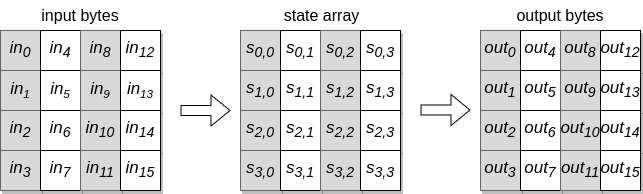
\includegraphics[width= 0.8\textwidth]{figure_5.3}\\
\caption{ AES input bytes, state array, and output bytes}
\label{fig:figure_5.3}
\end{figure}

The subscripts in Figure \ref{fig:figure_5.3} denote the position of the byte in the block. The usage of the terms "row" and "column" should be interpreted with this convention in mind.

The SubBytes operation replaces the value of each byte in the block. The mapping of values is performed using the mathematical process. The calculation of the transformation consists of two parts. The first part is the calculation of the multiplicative inverse in the field $GF(2^8)$. The second part is the calculation of the inverse of the affine transformation. The calculation of the multiplicative inverse is presented in Figure \ref{fig:figure_5.4}. The individual operations involved are defined:\\

\begin{equation}
\delta \equiv \begin{bmatrix}
1  & 0  & 1  & 0  & 0  & 0  & 0  & 0 \\
1  & 1  & 0  & 1  & 1  & 1  & 1  & 0  \\ 
1  & 0  & 1  & 0  & 1  & 1  & 0  & 0  \\
1  & 0  & 1  & 0  & 1  & 1  & 1  & 0  \\
1  & 1  & 0  & 0  & 0  & 1  & 1  & 0  \\
1  & 0  & 0  & 1  & 1  & 1  & 1  & 0  \\
0  & 1  & 0  & 1  & 0  & 0  & 1  & 0  \\
0  & 1  & 0  & 0  & 0  & 0  & 1  & 1  \\
\end{bmatrix}
\cdot
\begin{bmatrix}
x7 \\ x6 \\ x5 \\ x4 \\ x3 \\ x2 \\ x1 \\ x0 \\ 
\end{bmatrix}
=
\begin{bmatrix}
x7\oplus x5  \\
x7\oplus x6\oplus x4\oplus x3\oplus x2\oplus x1 \\
x7\oplus x5\oplus x3\oplus x2 \\
x7\oplus x5\oplus x3\oplus x2\oplus x1 \\
x7\oplus x6\oplus x2\oplus x1 \\
x7\oplus x4\oplus x3\oplus x2\oplus x1 \\
x6\oplus x4\oplus x1 \\
x6\oplus x1\oplus x0 \\
\end{bmatrix}
\\\\
\end{equation}

\begin{equation}
\delta ^-1 \equiv 
\begin{bmatrix}
1  & 1  & 1  & 0  & 0  & 0  & 1  & 0 \\
0  & 1  & 0  & 0  & 0  & 1  & 0  & 0 \\
0  & 1  & 1  & 0  & 0  & 0  & 1  & 0 \\
0  & 1  & 1  & 1  & 0  & 1  & 1  & 0 \\
0  & 0  & 1  & 1  & 1  & 1  & 1  & 0 \\
1  & 0  & 0  & 1  & 1  & 1  & 1  & 0 \\
0  & 0  & 1  & 1  & 0  & 0  & 0  & 0 \\
0  & 1  & 1  & 1  & 0  & 1  & 0  & 1 \\
\end{bmatrix}
\cdot
\begin{bmatrix}
x7 \\ x6 \\ x5 \\ x4 \\ x3 \\ x2 \\ x1 \\ x0 \\ 
\end{bmatrix}
=
\begin{bmatrix}
x7\oplus x6\oplus x5\oplus x1  \\
x6\oplus x2 \\
x6\oplus x5\oplus x1  \\
x6\oplus x5\oplus x4\oplus x2\oplus x1  \\
x5\oplus x4\oplus x3\oplus x2\oplus x1  \\
x7\oplus x4\oplus x3\oplus x2\oplus x1  \\
x5\oplus x4 \\
x6\oplus x5\oplus x4\oplus x2\oplus x0  \\
\end{bmatrix}\\
\end{equation}\\

% fig 5.4
\begin{figure}
\centering
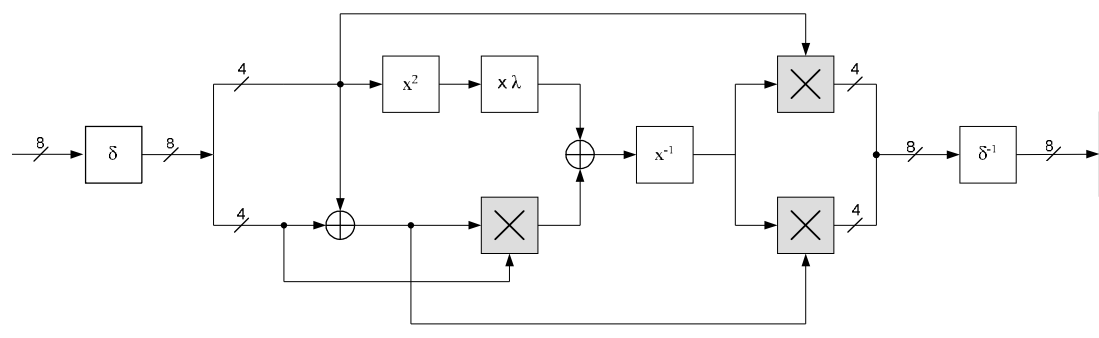
\includegraphics[width= 0.8\textwidth]{figure_5.4}\\
\caption{ Multiplicative inverse in $GF(2^8)$ }
\label{fig:figure_5.4}
\end{figure}

\begin{equation}
x^2 \equiv
\begin{bmatrix}
x3 \\
x3\oplus x2 \\
x2\oplus x1 \\
x3\oplus x1\oplus x0 \\
\end{bmatrix}
\end{equation}

\begin{equation}
x\lambda \equiv
\begin{bmatrix}
x2\oplus x0 \\
x3\oplus x2\oplus x1\oplus x0 \\
x3 \\
x2 \\
\end{bmatrix}\\
\end{equation}\\

\noindent
Additionally, the definition of multiplication is:\\
\begin{equation}
% \begin{split}
% \begin{aligned}
x\cdot y \equiv\\
\begin{bmatrix}
[(x3\oplus x1)(y3\oplus y1)]\oplus [(x2\oplus x0)(y3\oplus y1)]\oplus [(x3\oplus x1)(y2\oplus y0)]\oplus \\\oplus  (x1\cdot y1)\oplus (x0\cdot y1)\oplus (x1\cdot y0) \\\\
[(x3\oplus x1)(y3\oplus y1)]\oplus [(x2\oplus x0)(y2\oplus y0)]\oplus (x1\cdot y1)\oplus (x0\cdot y0) \\\\
(x1\cdot y1)\oplus (x0\cdot y1)\oplus (x1\cdot y0)\oplus (x3\cdot y3)\oplus (x2\cdot y3)\oplus (x3\cdot y2)\oplus (x2\cdot y2) \\\\
(x1\cdot y1)\oplus (x0\cdot y0)\oplus (x3\cdot y3)\oplus (x2\cdot y3)\oplus (x3\cdot y2) \\\\
\end{bmatrix}\\
% \end{split}
% \end{aligned}
\end{equation}\\

\noindent
Finally, we have the value mapping for the multiplicative inverse in $GF(2^4)$:\\
\begin{equation}
\begin{split}
x^{-1}(0000)= 0000, x^{-1}(0001)= 0001, x^{-1}(0010)= 0011, x^{-1}(0011)= 0010\\
x^{-1}(0100)= 1111, x^{-1}(0101)= 1100, x^{-1}(0110)= 1001, x^{-1}(0111)= 1011\\
x^{-1}(1000)= 1010, x^{-1}(1001)= 0110, x^{-1}(1010)= 1000, x^{-1}(1011)= 0111\\
x^{-1}(1100)= 0101, x^{-1}(1101)= 1110, x^{-1}(1110)= 1101, x^{-1}(1111)= 0100\\  
\end{split}
\end{equation}\\


The calculation of the inverse affine transformation takes one byte as input and computes the following operation:\\

\begin{equation}
AT^{-1} \equiv
\begin{bmatrix}
0  & 1  & 0  & 1  & 0  & 0  & 1  & 0 \\
0  & 0  & 1  & 0  & 1  & 0  & 0  & 1 \\
1  & 0  & 0  & 1  & 0  & 1  & 0  & 0 \\
0  & 1  & 0  & 0  & 1  & 0  & 1  & 0 \\
0  & 0  & 1  & 0  & 0  & 1  & 0  & 1 \\
1  & 0  & 0  & 1  & 0  & 0  & 1  & 0 \\
0  & 1  & 0  & 0  & 1  & 0  & 0  & 1 \\
1  & 0  & 1  & 0  & 0  & 1  & 0  & 0 \\
\end{bmatrix}
\cdot
\begin{bmatrix}
x7 \\
x6 \\
x5 \\
x4 \\
x3 \\
x2 \\
x1 \\
x0 \\
\end{bmatrix}
+
\begin{bmatrix}
0 \\
0 \\
0 \\
0 \\
0 \\
1 \\
0 \\
1 \\
\end{bmatrix}\\
\end{equation}\\

where $x_n$ is the n\ts{th} bit of the input byte. ShiftRows performs a one-byte rotation of the \nth{2} row, a two-byte rotation of the \nth{3} row, and a three-byte rotation of the \nth{4} row. 
 MixColumns multiplies each column by the matrix:\\

\begin{equation}\label{eq:mixcolumns}
\begin{bmatrix}
02 & 03 & 01 & 01 \\
01 & 02 & 03 & 01 \\
01 & 01 & 02 & 03 \\
03 & 01 & 01 & 02 \\
\end{bmatrix}_{10}\\
\end{equation}\\

\noindent
and the result replaces the initial column. Finally, the AddRoundKey performs bitwise XOR of the block and the round key.
The decryption operations execute the inverse process. Thus, the InvSubBytes performs the inverse substitution of the value of each byte. To calculate the inverse value, the byte first undergoes an affine transformation:\\

\begin{equation}
AT  \equiv
\begin{bmatrix}
1  & 0  & 1  & 0  & 0  & 0  & 0  & 0  &  \\
1  & 1  & 0  & 1  & 1  & 1  & 1  & 0  &  \\
1  & 0  & 1  & 0  & 1  & 1  & 0  & 0  &  \\
1  & 0  & 1  & 0  & 1  & 1  & 1  & 0  &  \\
1  & 1  & 0  & 0  & 0  & 1  & 1  & 0  &  \\
1  & 0  & 0  & 1  & 1  & 1  & 1  & 0  &  \\
0  & 1  & 0  & 1  & 0  & 0  & 1  & 0  &  \\
0  & 1  & 0  & 0  & 0  & 0  & 1  & 1  &  \\
\end{bmatrix}
\cdot
\begin{bmatrix}
x7 \\
x6 \\
x5 \\
x4 \\
x3 \\
x2 \\
x1 \\
x0 \\
\end{bmatrix}
+
\begin{bmatrix}
1 \\
1 \\
0 \\
0 \\
0 \\
1 \\
1 \\
0 \\
\end{bmatrix}\\
\end{equation}\\

\noindent
and then through an inverse multiplication in $GF(2^8)$.
The InvShiftRows performs the same rotations in the opposite direction (right), and the InvMixColumns multiplies by the inverse matrix of MixColumns:\\

\begin{equation} \label{eq:invmixcolumns}
\begin{bmatrix}
14 & 11 & 13 & 09 \\
09 & 14 & 11 & 13 \\
13 & 09 & 14 & 11 \\
11 & 13 & 09 & 14 \\
\end{bmatrix}_{10}\\
\end{equation}\\

\noindent
and the InvAddRoundKey is the same as the AddRoundKey.

In the key generation process, a matrix of constant values, called $Rcon$, is involved which is defined as: \\

\begin{equation} \label{eq:rcon}
    Rcon \equiv \begin{bmatrix}
01 & 02 & 04 & 08 & 10 & 20 & 40 & 80 & 1B & 36 \\
00 & 00 & 00 & 00 & 00 & 00 & 00 & 00 & 00 & 00 \\
00 & 00 & 00 & 00 & 00 & 00 & 00 & 00 & 00 & 00 \\
\end{bmatrix}_{16}\\
\end{equation}

\noindent
Each column of this matrix participates in the corresponding round key generation. (the \nth{1} in the \nth{1} round, the \nth{2} in the \nth{2}, etc.).
The key generation process is as follows:
To generate the first column of the new key, the last column of the previous key is selected, and a RotWord (see Figure \ref{fig:figure_5.5}) is performed. Then, each byte of the column undergoes the SubBytes process, and finally, this column, along with the \nth{1} column of the previous key and the corresponding column of the Rcon matrix, undergo bitwise XOR. The resulting column is the \nth{1} column of the new key.

 % fig 5.5
\begin{figure}
\centering
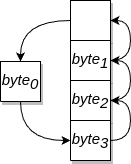
\includegraphics[width= 0.2\textwidth]{figure_5.5}\\
\caption{ The RotWord operation}
\label{fig:figure_5.5}
\end{figure}


The value of the \nth2 column is the result of the bitwise XOR of the \nth{2} column of the previous key with the \nth{1} column of the new key, the \nth{3} column's value is the result of the bitwise XOR of the \nth{3} column of the previous key with the \nth{2} column of the new key, and the \nth{4} column's value is the result of the bitwise XOR of the \nth{4} column of the previous key with the \nth{3} column of the new key. This process is repeated 10 times to produce 10 keys, one for each encryption round. The keys generated are passed to the AddRoundKey of the corresponding round. It is noteworthy that in decryption, the keys are provided in the reverse order compared to encryption.

\subsubsection*{Design Decisions}
Various parameters need to be taken into account, before commencing the design and implementation of this peripheral. Since the peripheral will operate as a slave of a processor, the interfaces between them, the communication protocol, and the individual technical details must be first defined.

In a processing system, the processor undertakes various tasks. Therefore, peripherals should be designed to operate with waiting states. In the case of CBC-AES-128, the peripheral should be in a waiting state until the processor provides it with the next input or command. Additionally, when an operation is completed and there is output available for the processor, the peripheral should have a way to notify the processor and wait until the processor consumes the peripheral's output.

For the communication protocol between the peripheral and the processor, both control signals driven by the processor and status signals driven by the peripheral are needed. These signals are designed, and their behavior is defined in a way that facilitates straightforward hardware design and straightforward management from the software side.

An important design decision is choosing the data transfer method between the peripheral and the memory. Many options exist, such as DMA, the peripheral switching between master and slave modes in the main bus, or direct access to the processor's registers (a Microblaze feature provided by Xilinx, called FSL, Fast Simplex Link). Ultimately, because the system is not multipacket, the processor does not process many packets simultaneously, and therefore there is no benefit in a peripheral taking over the data transfer, as during the data transfer, the processor will be blocked in a waiting state. Thus, the design decision is that the data transfer will be performed by the processor.

Finally, regarding the means of the peripheral notifying processor, there exist two options, polling and using interrupts. The polling method is implemented since due to the lack of multipacketing, the processor would be inactive while waiting for an interrupt.


\subsubsection*{Hardware Design}
The hardware design is organized hierarchically. At the lowest level, the internal operations of AES (ShiftRows, SubBytes, MixColumns, AddRoundKey) are implemented. These are used to implement the unit that executes one round of AES and another unit that executes one round of the key expansion. The complete key expansion unit is then implemented. Finally, at the top level, these subcomponents are integrated to implement the complete AES in CBC mode. Next, we elaborate on the hardware designs, in a bottom-up approach.

The implementation of ShiftRows and InvShiftRows is simply a permutation of their input bytes. The unit implementing the SBOX and its inverse (InvSBOX), receives a signal called EncDec which indicates whether the unit will operate in encryption or decryption mode. This design choice is made with resource reuse of the inverse multiplication $GF(2^8)$ in mind in order to optimize the area utilization of these components. The affine transform, inverse affine transform, and multiplicative inverse are designed using logic gates that directly implement their equations. Figure \ref{fig:figure_5.6} presents the block diagram of the unit. Due to the combined implementation of SBOX and InvSBOX, the implementation of SubBytes and InvSubBytes is also combined in a unit that accepts an EncDec signal that is passed down to these operations. The block diagram of the unit of SubBytes and InvSubBytes is shown in Figure \ref{fig:figure_5.7}.

 % fig 5.6
\begin{figure}[H]
\centering
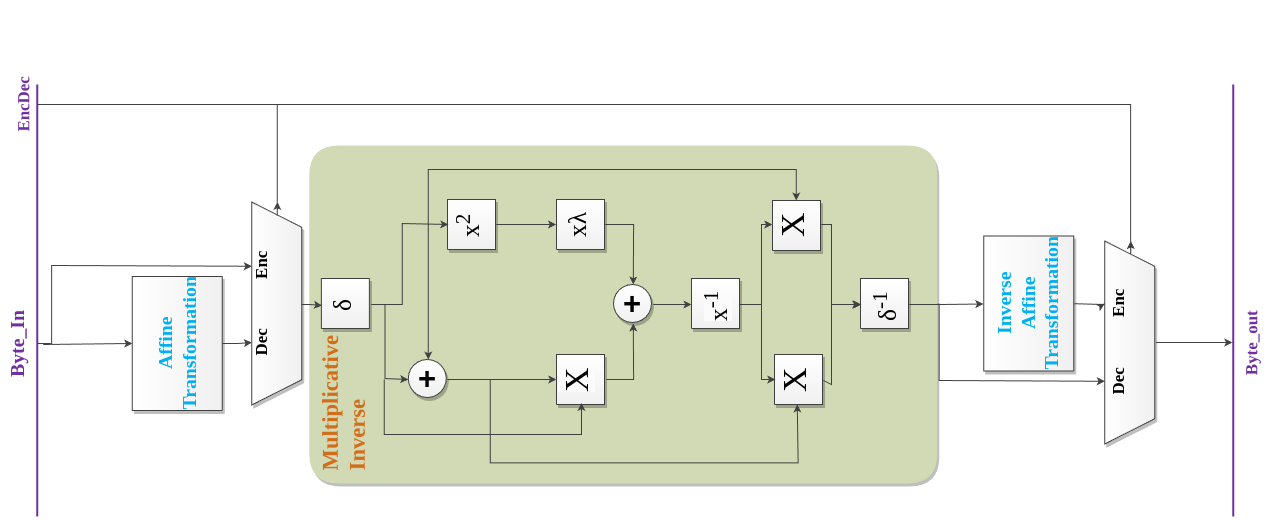
\includegraphics[width = 1.4\textwidth, angle=270,origin=c]{figure_5.6}\\
\caption{ Combined implementation of SBOX and InvSBOX }
\label{fig:figure_5.6}
\end{figure}


% fig 5.7
\begin{figure}
\centering
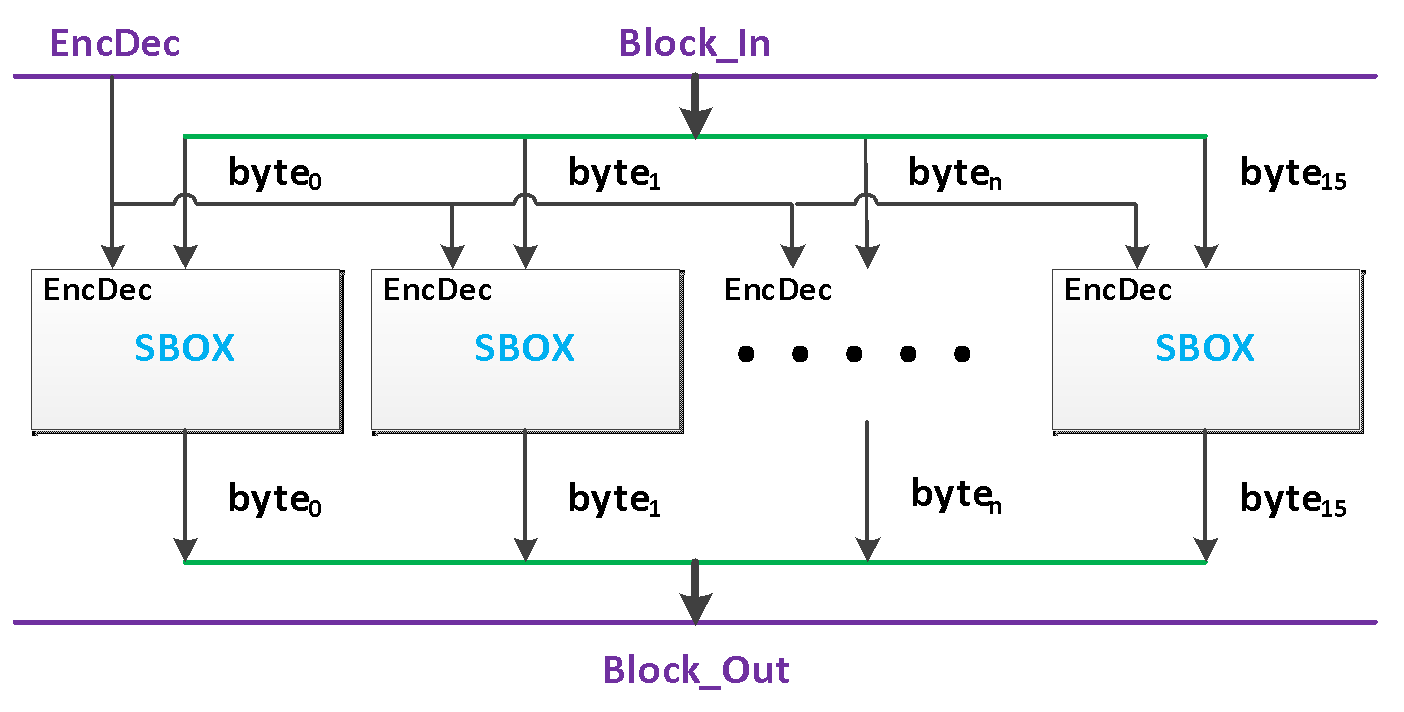
\includegraphics[width= 0.8\textwidth]{figure_5.7}\\
\caption{ Combined implementation of SubBytes and InvSubBytes }
\label{fig:figure_5.7}
\end{figure}

The operations MixColumns and InvMixColumns are implemented in a combined unit. The selection of the operation is specified using an EncDec signal. Because each column is processed independently of other columns, 4 subunits named MixOneColumn, one per column, are implemented to exploit parallelism and thus reduce latency. The block diagram of the combined MixColumns and InvMixColumns unit is presented in Figure \ref{fig:figure_5.8}.

% fig 5.8
\begin{figure}
\centering
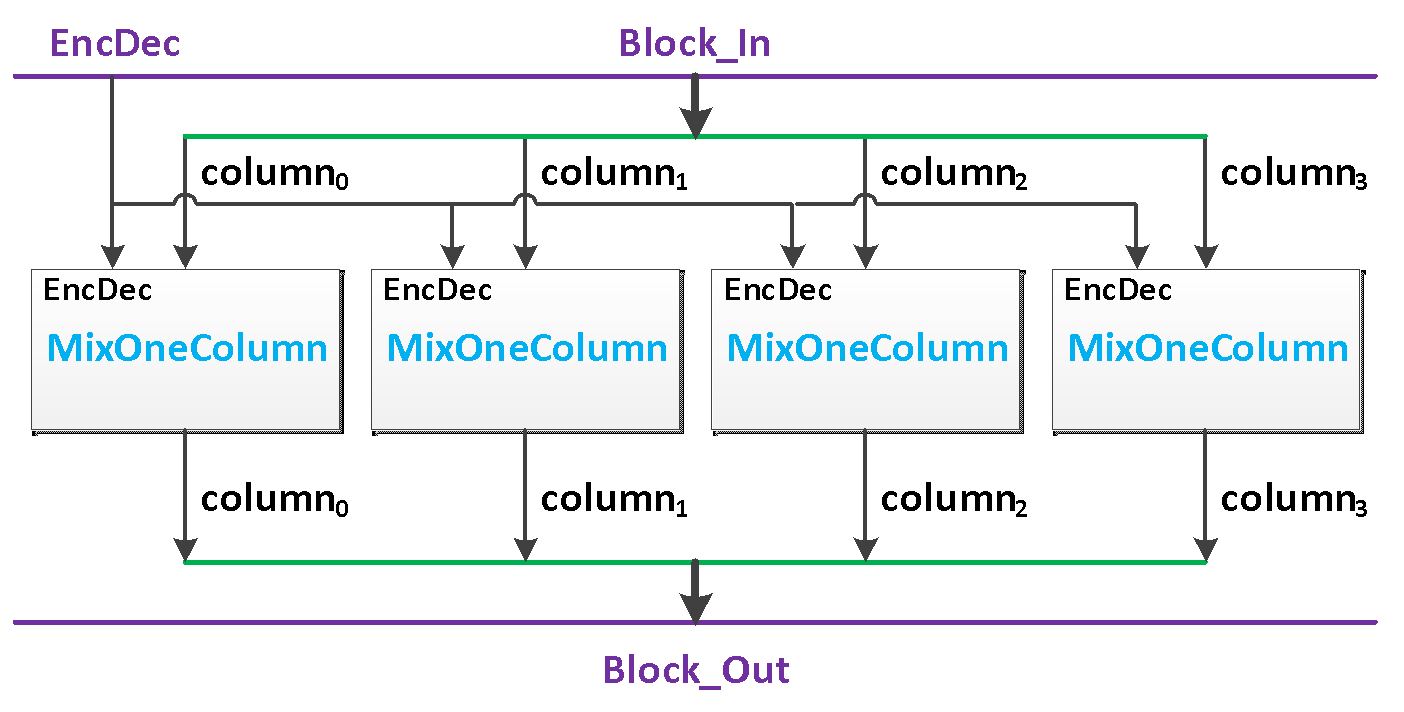
\includegraphics[width= 0.8\textwidth]{figure_5.8}\\
\caption{   Combined implementation of MixColumns and InvMixColumns}
\label{fig:figure_5.8}
\end{figure}

In each MixOneColumn, the column is multiplied by the matrix ~\ref{eq:mixcolumns} during encryption and by the matrix ~\ref{eq:invmixcolumns} during decryption. We observe that each byte of the column must be multiplied by the numbers $02$ and $03$ for encryption and by $14$, $11$, $13$, and $09$ for decryption. Thus, a unit named XTimes is created, which takes one byte as input and outputs its multiples of 2, 3, 9, 11, 13, and 14. The appropriate additions of the multiples are performed, and the final results are placed in the corresponding bytes of the output column. The implementation of MixOneColumn is presented in Figure \ref{fig:figure_5.9}. In this figure, to distinguish the outputs of XTimes, a suffix with the byte number is used (the signal x2\_0 means twice byte\ssc{0}, x14\_3 means 14 times byte\ssc{3}, and so on).

% fig 5.9
\begin{figure}[H]
\centering
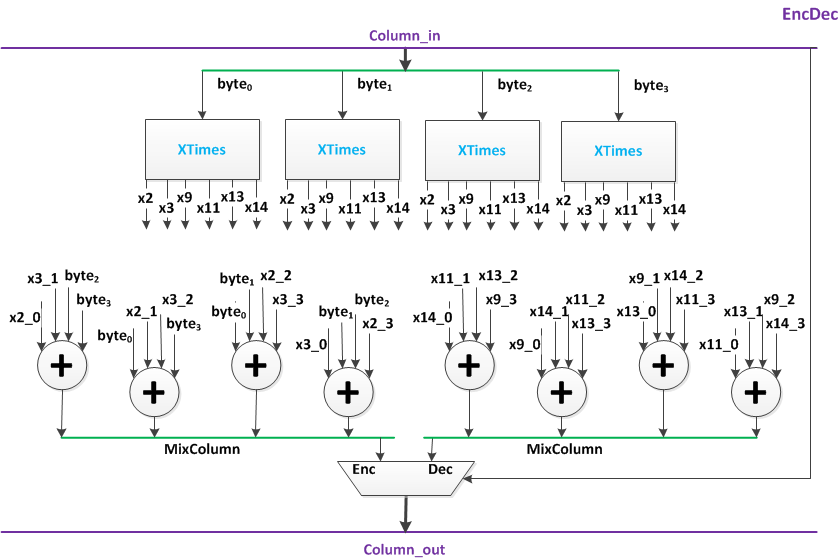
\includegraphics[width= 0.8\textwidth]{figure_5.9}\\
\caption{ Implementation of MixOneColumn}
\label{fig:figure_5.9}
\end{figure}

The implementation of XTimes is presented in Figure \ref{fig:figure_5.10}. The individual operations are characterized by the following equations: \\

\begin{equation}
\begin{split}
&3x=2x\oplus x,\\
&4x=2\cdot 2x,\\
&8x=2\cdot 4x,\\
&9x=x\oplus8x,\\
&10x=2x\oplus 8x,\\
&11x=10x\oplus x,\\
&12x=10x\oplus 2x,\\
&13x=12x\oplus x,\\
&14x=12x\oplus2x \\
\end{split}
\end{equation}\\

% fig 5.10
\begin{figure}
\centering
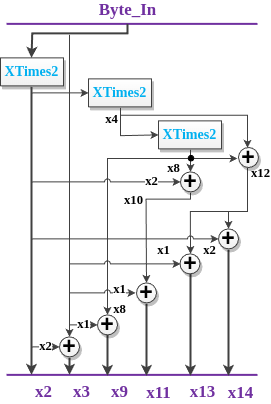
\includegraphics[width= 0.4\textwidth]{figure_5.10}\\
\caption{ Implementation of XTimes }
\label{fig:figure_5.10}
\end{figure}


In Figure \ref{fig:figure_5.11}, the unit for computing the double of XTimes, named XTimes2 is illustrated. This operation takes place in the $GF(2^8)$ field and is defined as follows: For the input byte, a left shift is performed first. If the MSbit of the input byte is 0, then the shift does not overflow, and the output is given by the shifted byte. Otherwise, if there is overflow, the value $1B_{16}$ must be added (via XOR) to the shifted byte.

% fig 5.11
\begin{figure}
\centering
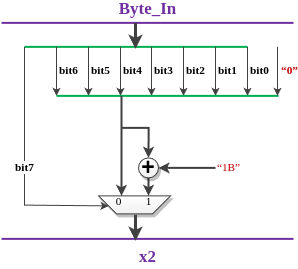
\includegraphics[width= 0.5\textwidth]{figure_5.11}\\
\caption{ Implementation of XTimes2 }
\label{fig:figure_5.11}
\end{figure}


The last unit in an AES round is the AddRoundKey, which is simply a bitwise XOR between the block and the current round key. The key is provided as input, and ultimately, AddRoundKey is a bitwise XOR of length 128 bits.

Finally, combining the above units, a unit for computing a round of AES-128 is implemented. Its inputs are the input block, the key of the current round, the EncDec signal for selecting encryption or decryption mode, and a LastRound signal indicating if the operation is currently executing the last AES round. LastRound is needed because the last round of AES-128 differs from the preceding 9 rounds. The output of the unit is the processed block. The block diagram of the design is presented in Figure \ref{fig:figure_5.12}. The differences between encryption and decryption are (as shown in Figure \ref{fig:figure_5.2}):
\begin{outline}[enumerate]
\1 Execution of ShiftRows versus execution of InvShiftRows
\1 Execution of SubBytes  versus execution of InvSubBytes
\1 Execution of MixColumns  versus execution of InvMixColumns
\1 Execution of AddRoundKey after MixColumns in encryption, and vice versa for decryption.
\end{outline}
The first difference is implemented using a MUX, which selects between the output of ShiftRows or InvShiftRows based on the EncDec signal. The second and third differences are already implemented within the common units of SubBytes and MixColumns respectively, using the EncDec signal. The fourth difference is implemented using two AddRoundKey units, one placed before MixColumns and one placed after. When in encryption mode, the first AddRoundKey is bypassed using a MUX, while the second one is used. In decryption, the second one is bypassed with a MUX while the first one is used.

The difference in the final rounds of encryption and decryption from the other 9 is (as shown in Figure 5.2) that the MixColumns and InvMixColumns operations are not performed respectively. Because these two operations are implemented in one unit, only one bypass MUX is needed with the LastRound signal as the selection signal.

% fig 5.12
\begin{figure}
\centering
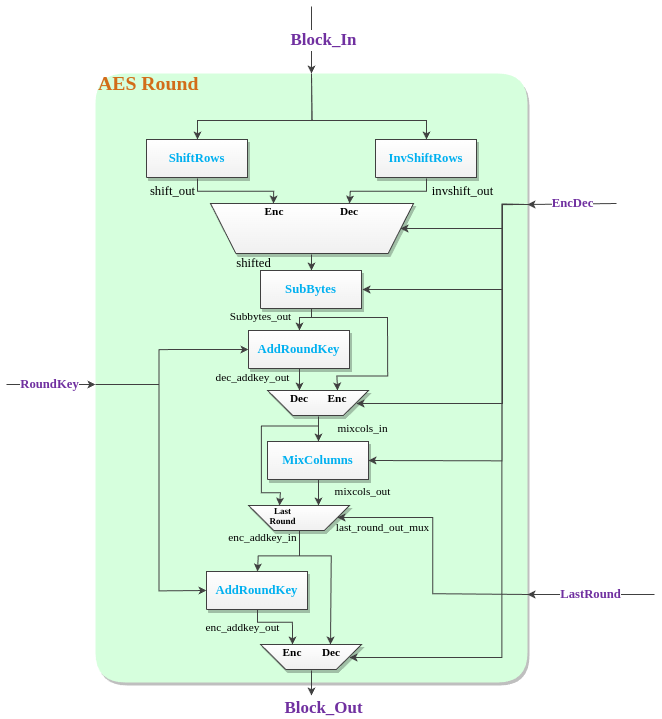
\includegraphics[width= 1\textwidth]{figure_5.12}\\
\caption{  Implementation of one round of AES-128 }
\label{fig:figure_5.12}
\end{figure}

For the calculation of the round keys, first, a unit named KeyScheduleRound is implemented for computing the next round key. The key calculation is identical for encryption and decryption, with the only difference being that during decryption, the keys are provided to the AES rounds in the reverse order from the order in which they are calculated. This difference is managed at a higher level of the design. The block diagram of the KeyScheduleRound is presented in Figure \ref{fig:figure_5.13}.

The KeyScheduleRound unit takes as inputs the key of the previous round and the Rcon value corresponding to the current round and outputs the key generated for the current round. In the design, 4 SBOX units are used, each for each of the 4 bytes of the last column of the input key. Because the inverse operation InvSBOX is not needed, a separate SBOX unit is implemented, which performs only the calculations for multiplicative inverse and inverse affine transform, to save on area utilization.

% fig 5.13
\begin{figure}
\centering
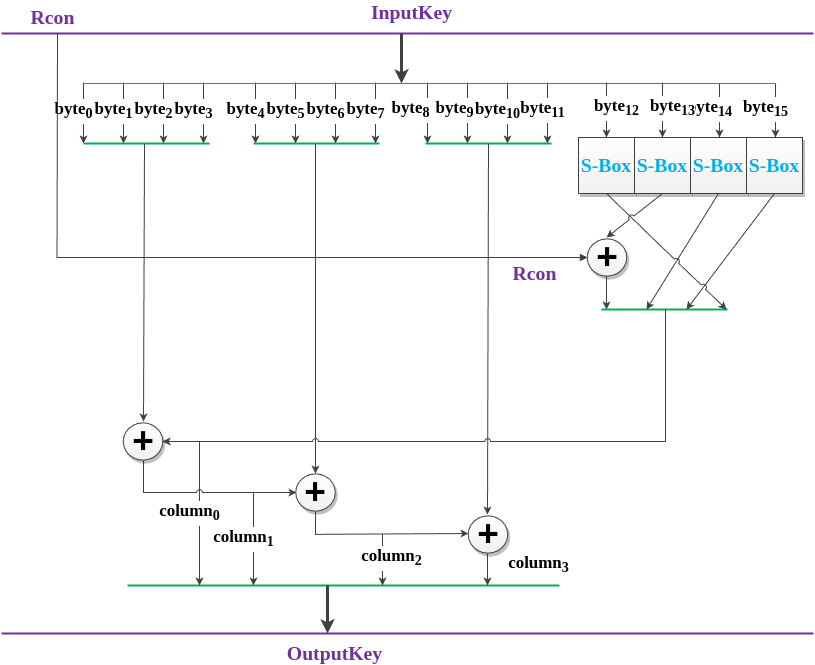
\includegraphics[width= 0.8\textwidth]{figure_5.13}\\
\caption{ Implementation of one round of AES-128 Key Scheduler }
\label{fig:figure_5.13}
\end{figure}

The computations executed are as follows: first, the substitution through the SBOX of the last column of the input key is performed, and the result undergoes a RotWord, which is simply a permutation of the bytes. After RotWord, a bitwise XOR with the value of Rcon is performed. From Figure \ref{eq:rcon}, we observe that the last 3 bytes of each column of Rcon are zero, so they do not affect the bitwise XOR. Thus, only the first byte of Rcon is needed as input, and a bitwise XOR of 8 bits instead of 32 bits is sufficient. The first column of the output key is the processed last column of the input. The second output column is calculated with a bitwise XOR between the first input column and the processed last input column, the third with a bitwise XOR of the second output column with the second input column, and the fourth with the third output and the third input column.

Using KeyScheduleRound, the unit for computing all round keys, named KeyScheduler, is implemented. Its block diagram is presented in Figure \ref{fig:figure_5.14}. Its inputs are the initial key, a round counter indicating the current round, and the signal FirstRound indicating that we are in the first round. The output provides the current round key at any given time. The unit contains a KeyScheduleRound subunit and an Rcon subunit which takes as input the round counter and outputs the first byte of the corresponding column of Rcon (since the others are $'00'$) and feeds this value to the KeyScheduleRound.

% fig 5.14
\begin{figure}
\centering
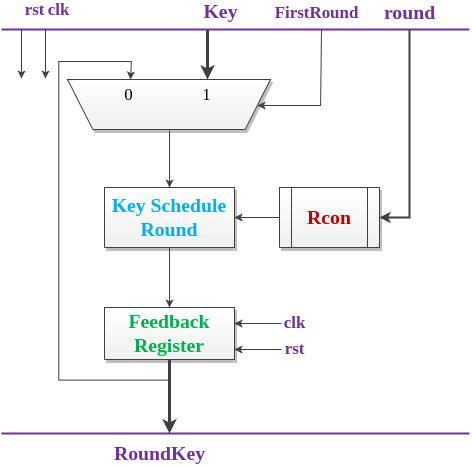
\includegraphics[width= 0.6\textwidth]{figure_5.14}\\
\caption{ Implementation of the AES-128 Key Scheduler }
\label{fig:figure_5.14}
\end{figure}


The value of the first derived key depends on the value of the initial key while the value of any other derived key depends on the directly preceding derived key. The FirstRound signal helps differentiate between the two scenarios. It is used to route either the initial key or the preceding derived key through the feedback loop back as input to the KeyScheduleRound unit.

Finally, the peripheral of CBC-AES-128 is implemented. Its block diagram is presented in Figure \ref{fig:figure_5.15}. Its inputs are:
\begin{outline}
    \1 Block\_in: the current message block
    \1 IV: the initialization vector
    \1 Key: the cryptographic key
    \1 Start\_new: a control signal denoting an instruction for a new encryption/decryption operation
    \1 Next\_block: a control signal indicating that the next input block is present at the Block\_in
    \1 EncDec: a control signal for selecting between encryption and decryption operations
    \1 clk: the system's clock signal
    \1 rst: the system's reset signal
\end{outline}
As outputs, the peripheral provides the output block and a control signal named 'ready' indicating the end of block processing, i.e., that the output block is ready.

In Figure \ref{fig:figure_5.15} the colored area on the left outlines the parts that implement the CBC operation. The part in the middle is the AES operation, and the part on the right is the key generation operation. In the bottom right, the peripheral's control circuit is presented, alongside its input and output signals.

The CBC implementation uses two bitwise XORs, one applied at the input block before it is passed to the AES operation and one applied at the output of the AES operation. The first XOR gets selected by a MUX when in encryption mode, while the second XOR is selected in decryption mode. The second input of both XORs is determined based on the combination of the current block number and if the operation is encryption or decryption. When we are processing the first block, the IV is provided to the XORs. For any other block, if we are in encryption mode, the value of the previous AES output is provided, while if in decryption mode, the value provided is the previous input block. These options are implemented with the appropriate placement of registers, MUXes, and the needed control signals managed by the control circuit.

% fig 5.15
\begin{figure}
\centering
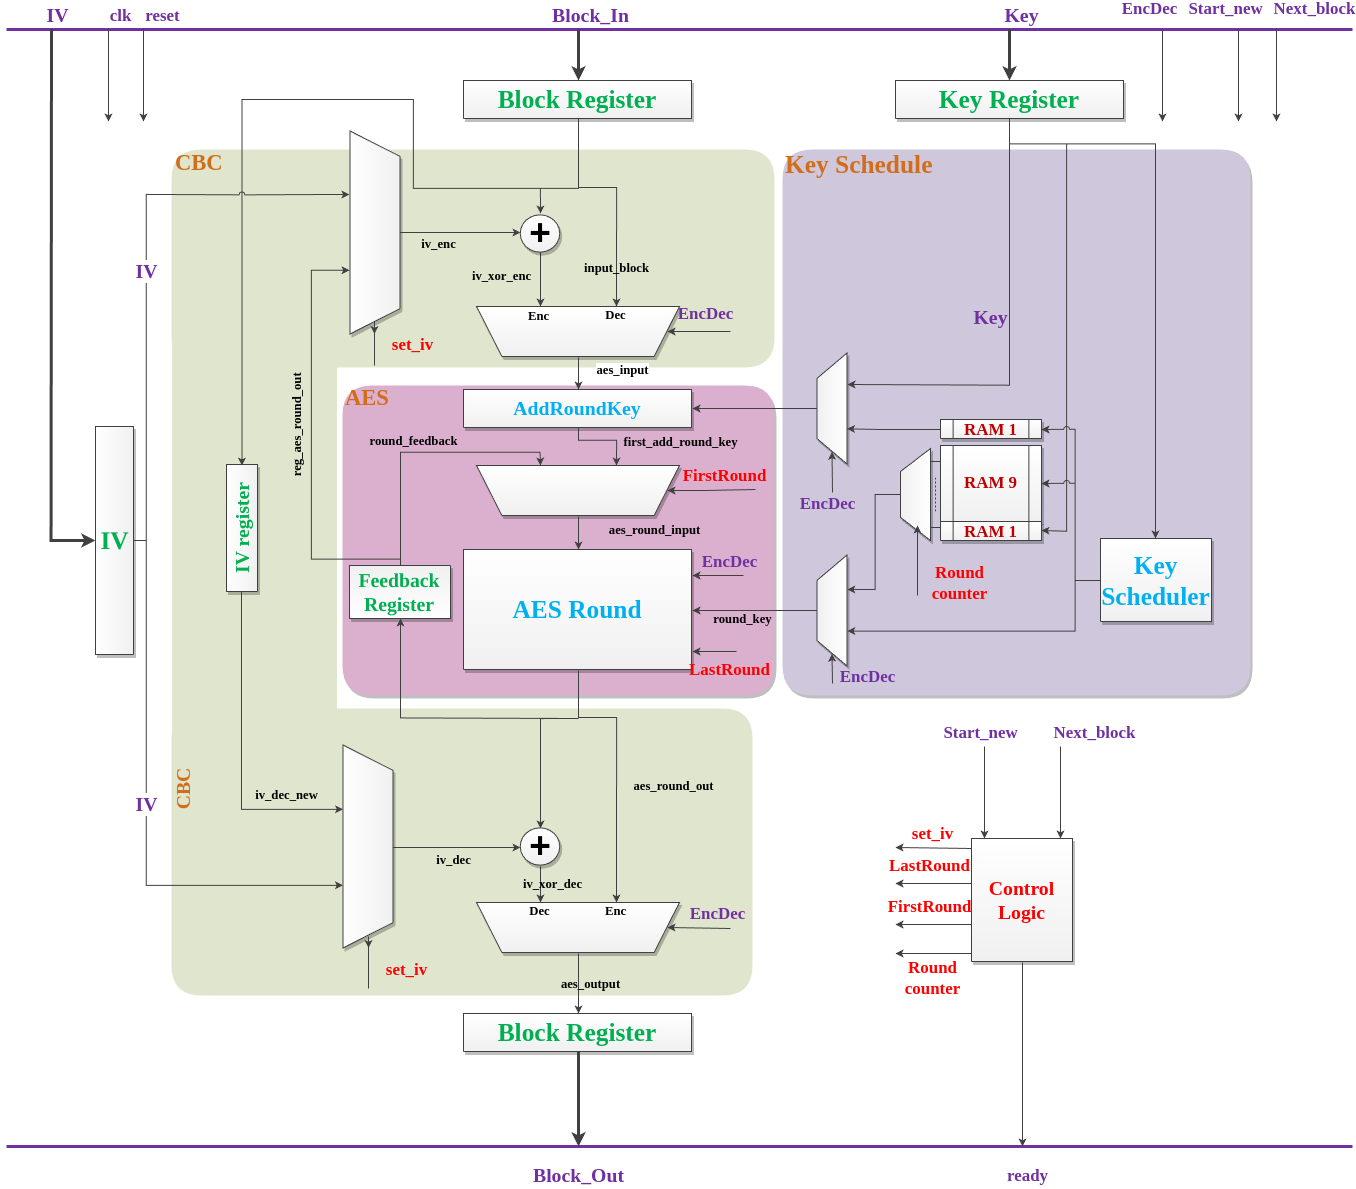
\includegraphics[width= 0.8\textwidth]{figure_5.15}\\
\caption{ Implementation of CBC-AES-128 }
\label{fig:figure_5.15}
\end{figure}


The AES part first needs to perform an AddRoundKey to the input before continuing with the 10-round processing, as shown in Figure \ref{fig:figure_5.2}. The 10 AES rounds are implemented by using a feedback loop around the AES Round unit. The signal FirstRound selects which value will be used in the AES Round, either the result of the AddRoundKey or the previous output via feedback.

The core of the key generation operation is a KeyScheduler unit. When in encryption mode, where the keys must be provided in the order they are generated, the KeyScheduler directly provides its output to the AES Round, and the initial AddRoundKey is given the initial key from the input. In decryption mode, where the keys must be provided in the reverse order of the order they get generated, the last key must be given to the initial AddRoundKey, which requires the computation and storing of all the keys in advance. For this purpose, 11 registers are used as the key storage. The first 10 registers are populated by the KeyScheduler starting from the last register and in reverse order. This way the keys are stored in reverse order and are mapped correctly with their respective rounds. The initial input key is placed in the last (\nth{11}) register. Finally, the first register is connected directly to the AddRoundKey to provide the last derived key, while the other registers are selected by a MUX based on the round counter to be routed to the AES Round.

The control circuit receives the signals Start\_new and Next\_Block and provides the output signal ready and the internal control signals set\_iv (used for IV selection), LastRound, FirstRound, and Round\_counter, which is the counter indicating the current round. The control circuit is described by the FSM shown in Figure ~\ref{fig:figure_5.16}:

% fig 5.16
\begin{figure}
\centering
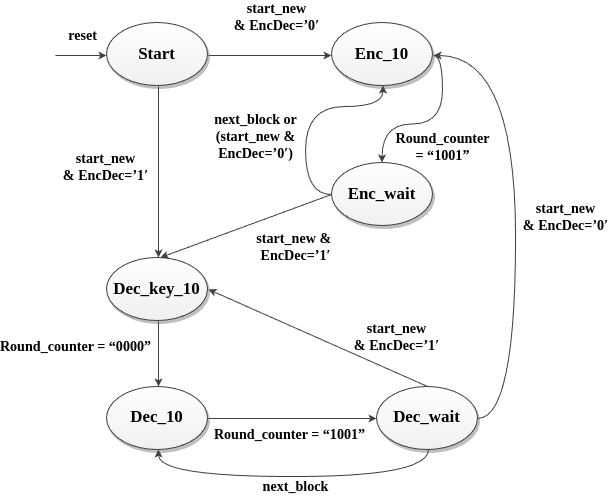
\includegraphics[width= 0.8\textwidth]{figure_5.16}\\
\caption{ The control FSM of CBC-AES-128 }
\label{fig:figure_5.16}
\end{figure}


Upon each reset, the FSM transitions to the initial Start state, where it waits for a start\_new signal. When start\_new arrives and depending on the value of the EncDec signal, it transitions to either encryption mode (EncDec='0') or decryption mode (EncDec='1'). Before a start\_new signal is issued, the key, the IV, and the first block of the message must be already provided at the module's inputs.

Encryption mode operates using two states. In the state Enc\_10, the 10 encryption rounds of AES are executed, and when finished it transitions to the Enc\_Wait state, where the peripheral waits. The transition between the two is implemented using a comparator that compares the Round\_Counter with the value "1001" (counting starts from 0, so a total of 10 rounds are counted). While in Enc\_Wait state, the peripheral waits for either the next block of the same message, indicated by the next\_block signal, or the start of a new message indicated by the start\_new signal. When a next\_block is received, the FSM returns back to Enc\_10 to process the new block. If start\_new arrives, the next FSM state depends on the value of EncDec. If  EncDec is '0', the FSM transitions to the Enc\_10  state in order to encrypt the first block of the new message, while if EncDec is '1', the FSM transitions to the Dec\_Key\_10 state, which is the first stage of the decryption operation.

In decryption mode, we have three states: Dec\_Key\_10, where all the keys first are generated and stored, Dec\_10, where the 10 decryption rounds of AES are executed, and Dec\_Wait, which is a waiting state that serves a similar purpose to Dec\_Wait. The keys must be generated once for every new message, thus Dec\_Key\_10 only takes place once at the start of the decryption process and there is no need to regenerate them on the arrival of every new block since the keys are kept in the key registers.

In Dec\_Key\_10, the Round\_Counter starts from the value "1001" so that the appropriate key registers are selected and traversed in reverse order. When Round\_Counter reaches 0, the decryption of the first block can commence by transitioning to state Dec\_10. The Round\_Counter gets increased in every round, and, after executing the 10 decryption rounds, Round\_Counter is "1001". At this point the FSM transitions to the waiting state Dec\_Wait. Dec\_Wait is identical to Enc\_Wait except from the fact that state transitions differ.

\subsection{HMAC-SHA1-96}
\subsubsection*{Algorithm Specification}
HMAC-SHA1-96 is a MAC algorithm that utilizes the cryptographic hash algorithm SHA1. The number 96 in the name indicates how many bits of the output are used. The mathematical formulation of HMAC is:

\begin{equation}
HMAC(K, text)_t=H[(K_0\oplus opad) || H((K_0\oplus ipad) || text)]_t
\end{equation}

\noindent
where:
\begin{outline}
\1 $text$ represents the input text,
\1 $H$ is the hash function used (in this case it is SHA1),
\1 $K$ is the key,
\1 $K_0$ is the key after preprocessing,
\1 $ipad$ is the repetition of the byte $[36]_{16}$, with a total size equal to the block size of the hash function,
\1 $opad$ is the repetition of the byte $[5C]_{16}$, with a total size equal to the block size of the hash function,
\1 $||$ denotes concatenation,
\1 $t$ is the size of the received output.
\end{outline}\\

\noindent
Figure \ref{fig:figure_5.17}, presents the HMAC operation schematically.

% fig 5.17
\begin{figure}[H]
\centering
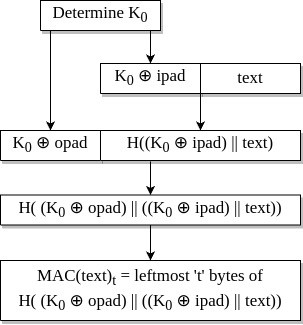
\includegraphics[width= 0.5\textwidth]{figure_5.17}\\
\caption{ The HMAC algorithm}
\label{fig:figure_5.17}
\end{figure}

HMAC has a preprocessing phase, where the value $K_0$ gets generated from the key $K$. The process differs depending on the size of key $K$ and the block size of $H$. When the size of $K$ matches the block size of $H$, $K$ simply takes the value of $K_0$. If the size of $K$ is smaller than the size of $H$, a padding of '0' bits is applied, while if larger, $K$ is first transformed through $H$ to produce $K_0$.

The SHA1 algorithm has an output size of 160 bits. It divides its input into 512-bit blocks and padding is applied for inputs whose size is not a multiple of 512 bits. It executes 80 iterations to process each input block. The algorithm is described in Algorithm \ref{alg:hmac_pre}, where $N$ is the number of input blocks, $M^i$ is the $i\ssc{th}$ input block and:

\begin{equation}
f_t(x,y,z) \equiv 
\begin{cases}
      M_t^{(i)} & 0 \leq t \leq 15\\
      ROTL^1(W_(t-3)\oplus W_(t-8)\oplus W_(t-14)\oplus W_(t-16)) & 16 \leq t \leq 79
\end{cases} \end{equation} \label{eq:f_t}


\begin{equation}
K_t \equiv 
\begin{cases}
    5a827999 & 0 \leq t \leq 19\\ 
    6ed9eba1 & 20 \leq t \leq 39\\ 
    8f1bbcdc & 40 \leq t \leq 59 \\
    ca62c1d6 & 60 \leq t \leq 79 
\end{cases} \end{equation}\label{eq:K_t}

SHA1 input padding includes two fixed fields: its first bit which takes the value '1', and the last 64 bits, which contain the original message's size expressed in bits in binary representation. The remaining bits in between are set to '0'. The total number of these '0's is chosen so that the original message together with the padding is a multiple of 512 bits.

\subsubsection*{Design Decisions}
The design decisions for the peripheral HMAC-SHA1-96 are the same as those for CBC-AES-128.

\subsubsection*{Hardware Design}
Algorithm \ref{alg:hmac_pre} is implemented in hardware. Firstly, the sha1\_core unit is implemented, which handles the processing of the 80 iterations of SHA1 for one block. Using this unit, the sha1 unit is designed, which computes the SHA1 hash of a complete input message. Finally, using the sha1 unit, the HMAC-SHA1-96 algorithm is implemented. The implementation assumes that the input is a multiple of 512 bits, and the padding, if needed, has been added beforehand. It is also assumed that any preprocessing of the key, if necessary, has already been done. All units are explained in detail below.

\begin{algorithm}[H]
\caption{HMAC Preprocessing}\label{alg:hmac_pre}
\begin{algorithmic}[1]
\Procedure{HMAC\_Preprocessing}{$N,M$}
% \Require $n \geq 0$
% \Ensure $y = x^n$

\Statex   \LeftComment{1} {Initialize $H$}
% \State $(H_0^{(0)}, H_1^{(0)}, H_2^{(0)}, H_3^{(0)}, H_4^{(0)}) \gets 
% (\texttt{67452301}_{16},
% \texttt{EFCDAB89}_{16},
% \texttt{98BADCFE}_{16},
% \texttt{10325476}_{16},
% \texttt{C3D2E1F0}_{16})$ 

\State $H_0^{(0)} \gets \texttt{67452301}_{16}$ \label{hmac:init_H}
 \State $H_1^{(0)} \gets \texttt{EFCDAB89}_{16}$
\State  $H_2^{(0)} \gets \texttt{98BADCFE}_{16}$
 \State $H_3^{(0)} \gets \texttt{10325476}_{16}$
 \State $H_4^{(0)} \gets \texttt{C3D2E1F0}_{16}$

\\
\For{\texttt{$1 \leq i \leq N$}}
    \Statex   \LeftComment{2} {Prepare the message schedule $\{W_t\}$}
    \State $W_t =
    \begin{cases}
      M_t^{(i)} & \text{$0 \leq t \leq 15$}\\
      ROTL^1(W_(t-3)\oplus W_(t-8)\oplus W_(t-14)\oplus W_(t-16)) & \text{$16 \leq t \leq 79$}\\
    \end{cases}
    $\label{hmac:wt} \\


    \Statex   \LeftComment{2} {Initialize the five working variables, $a, b, c, d,$ and $e$, with the $(i-1)$\ts{st} hash value:}
    \State $(a,b,c,d,e) \gets (H_0^{(i-1)},H_1^{(i-1)},H_2^{(i-1)},H_3^{(i-1)},H_4^{(i-1)})$ \label{hmac:assign3}
    % \State $a \gets H_0^{(i-1)}$;
    % $b \gets H_1^{(i-1)}$; 
    % $c \gets H_2^{(i-1)}$;
    % $d \gets H_3^{(i-1)}$;
    % $e \gets H_4^{(i-1)}$;
    \For{\texttt{$0 \leq t \leq 79$}}
        \State $T \gets ROTL^{5}(a)+f_t(b,c,d)+e+ K_t+ W_t$ \label{hmac:T}
        \State $(e,d,c,b) \gets (d,c,ROTL^{30}(b),a)$ \label{hmac:asign1}
        % \State $e \gets d$
        % \State $d \gets c$
        % \State $c \gets ROTL^{30}(b)$
        % \State $b \gets a$
        \State $a \gets T$
    \EndFor\\
    \Statex   \LeftComment{2} {Compute the i\ts{th} intermediate hash value $H^{(i)}$}
    \State $(H_0^{(i)},H_1^{(i)}, H_2^{(i)}, H_3^{(i)}, H_4^{(i)}) \gets
            (a + H_0^{(i-1)},b + H_1^{(i-1)},c + H_2^{(i-1)},d + H_3^{(i-1)},e + H_4^{(i-1)})$

    % \State $H_0^{(i)} \gets a + H_0^{(i-1)}$
    % \State $H_1^{(i)} \gets b + H_1^{(i-1)}$
    % \State $H_2^{(i)} \gets c + H_2^{(i-1)}$
    % \State $H_3^{(i)} \gets d + H_3^{(i-1)}$
    % \State $H_4^{(i)} \gets e + H_4^{(i-1)}$


    \EndFor\\

    \State \Return $( H_0^{(N)} || H_1^{(N)} || H_2^{(N)} || H_3^{(N)} || H_4^{(N)} )$ \label{hmac:asign2}
\EndProcedure
\end{algorithmic}
\end{algorithm}


For the calculation of $W_t$, the subunit shown in Figure \ref{fig:figure_5.18} is implemented. It acts as a shift register, where the output is taken from its head. Initially, the 16 registers are populated with values from the corresponding parts of the input block, with the rightmost register assigned to the \nth{1} block portion. Thus, for the first 16 cycles, the subunit outputs the parts of the input block. To compute the next W\ssc{t}, a bitwise XOR of W\ssc{t-3}, W\ssc{t-8}, W\ssc{t-14}, and W\ssc{t-16} is used, and the result is left-shifted by 1 bit. The new value of W\ssc{t} is then placed in the tail of the registers. Therefore, from the \nth{17} cycle onwards, the output corresponds to the calculated W\ssc{t} according to the second branch of the calculation in line~\ref{hmac:wt} in algorithm ~\ref{alg:hmac_pre}.

% fig 5.18
\begin{figure}[H]
\centering
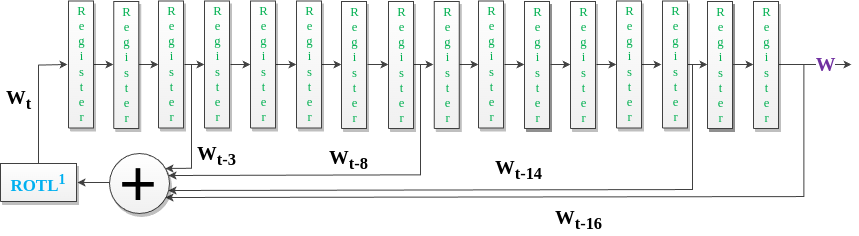
\includegraphics[width= 0.9\textwidth]{figure_5.18}\\
\caption{ SHA1 message schedule }
\label{fig:figure_5.18}
\end{figure}


The implementation of sha1\_core is depicted in Figure \ref{fig:figure_5.19}. Its inputs are the input block, the values $H_0^{(i-1)}, H_1^{(i-1)}, H_2^{(i-1)}, H_3^{(i-1)}, H_4^{(i-1)}$, and the clock ($clk$) and reset ($rst$) signals. The $H$ values are also needed as inputs because, as can be observed in the pseudocode in Algorithm \ref{alg:hmac_pre}, the new $H$ values are calculated using the previous ones. Thus, as will be explained in the sha1 unit description, there is an external feedback loop from the output of the sha1\_core into $H_0^{(i)}, H_1^{(i)}, H_2^{(i)}, H_3^{(i)}, H_4^{(i)}$. sha1 outputs the computed hash value and a signal hash\_rd which indicates that the processing of this block has finished.

% fig 5.19
\begin{figure}[H]
\centering
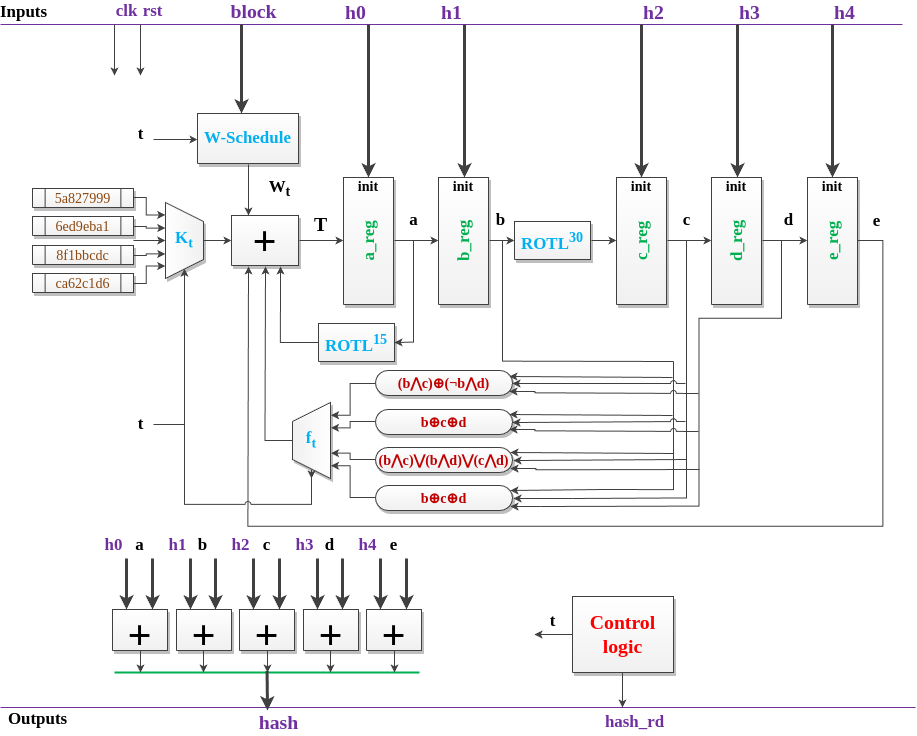
\includegraphics[width= 0.8\textwidth]{figure_5.19}\\
\caption{ sha1\_core module implementation }
\label{fig:figure_5.19}
\end{figure}


In Figure \ref{fig:figure_5.19}, the variable $t$ corresponds to the number of current iterations. The 5 registers connected in series (a\_reg to e\_reg) implement the assignments in line ~\ref{hmac:asign1}. The calculation of line ~\ref{hmac:T} is broken down to:

\begin{outline}
    \1 The calculation of $f_t$ (\ref{eq:f_t}) is performed through four segments of digital logic and a multiplexer among these four. The MUX selection is based on $t$
    \1 The signal $K_t$ (\ref{eq:K_t}) is assigned one of the four constant values depending on the value of $t$
    \1 The $W_t$ is computed by the W-Schedule unit
    \1 $ROTL5(a)$ is calculated, and all the above, along with $e$, are fed into an addition unit whose output is the value of $T$ 
    \1 the value of $T$ is stored into the $a\_reg$ in order to implement the final assignment $a = T$
\end{outline}

The output values (line ~\ref{hmac:asign2}) are computed using adders. The control logic includes a counter that is initialized to '0' with every rst and has a maximum value of '79', which keeps until a new rst signal is given. The value of $t$ corresponds to the value of this counter. Furthermore, the control logic raises the output signal hash\_rd when the counter reaches the value '79' to indicate that all iterations have been executed.

% fig 5.20
\begin{figure}[H]
\centering
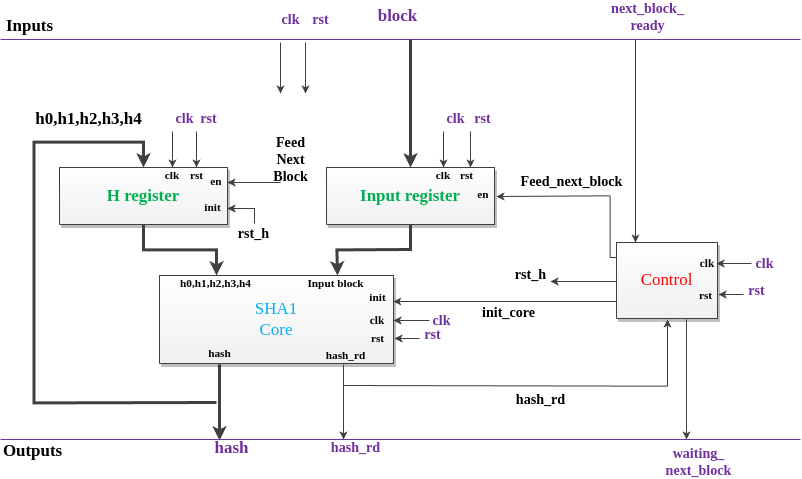
\includegraphics[width= 0.8\textwidth]{figure_5.20}\\
\caption{ sha1 module implementation}
\label{fig:figure_5.20}
\end{figure}

The sha1 unit takes as input the message's current block, the control signal next\_block\_ready which notifies the unit that a new block is available at its input, and the clock (clk) and reset (rst) signals. It outputs the result of the hash computation, the hash\_rd signal indicating the end of hash computation for the current block, and a waiting\_next\_block signal indicating that the unit is ready to accept a new block at its input. The block diagram of the implementation is shown in Figure \ref{fig:figure_5.20}.

The design consists of a sha1\_core, two registers, and a control unit. The input register serves as a buffer that holds the input block, allowing a new block to be placed at the unit's input without affecting the ongoing operation. The H register is used to feed back the values $H_0^{(i-1)}, H_1^{(i-1)}, H_2^{(i-1)}, H_3^{(i-1)},$ and $H_4^{(i-1)}$ for processing the next block, which implements the assignments in line ~\ref{hmac:assign3}.

% fig 5.21
\begin{figure}
\centering
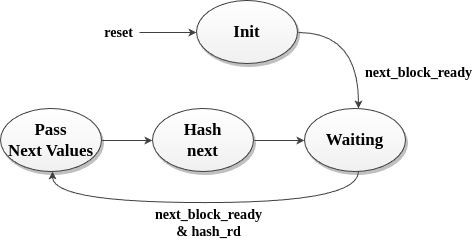
\includegraphics[width= 0.6\textwidth]{figure_5.21}\\
\caption{  sha1 control FSM }
\label{fig:figure_5.21}
\end{figure}

The operation of the control unit is described through the FSM diagram in Figure \ref{fig:figure_5.21}. For starting a hash computation of a new message, a reset signal needs to be issued that places us in the Init state. In this state, the H register is set to the initial values (line ~\ref{hmac:init_H}) and initializes the sha1\_core unit with the internal signal Init\_core. When entering the Init state, the waiting\_next\_block is issued.

After the first block is provided at the input the the next\_block\_ready signal is issued and that transitions the FSM to the Waiting state where the 80 iterations are executed for the first block. In this state, the control unit waits for the sha1\_core to finish processing, which is indicated by the hash\_rd signal, and for the next\_block\_ready signal to be given (after placing the next block at the input). When both conditions are met, the FSM transitions to the Pass Next Values state, where a pulse of the internal signal feed\_next\_block is issued so that the new values of $H$ and the next block are provided to the sha1\_core input. After one clock cycle, the FSM transitions to the Hash next state, where the sha1\_core has taken the new values at its inputs, and then automatically transitions to the Waiting state where the 80 iterations are executed for the current block. This process repeats until all blocks are provided.

The last unit implemented is the hmac\_sha1\_96, whose block diagram is shown in Figure \ref{fig:figure_5.22}. At its input, it receives the key, one message block msg\_block, the control signals next\_block and msg\_done, and the clock and reset signals. The next\_block signal is used to indicate that the next block is at the msg\_block input, while the msg\_done signal indicates that we are providing the last block of the message. Its outputs include the computed MAC and the signals waiting\_nxt and ready. The waiting\_nxt signal indicates that the unit is ready to accept a new block at its input, and ready indicates the end of the MAC computation.

% fig 5.22
\begin{figure}
\centering
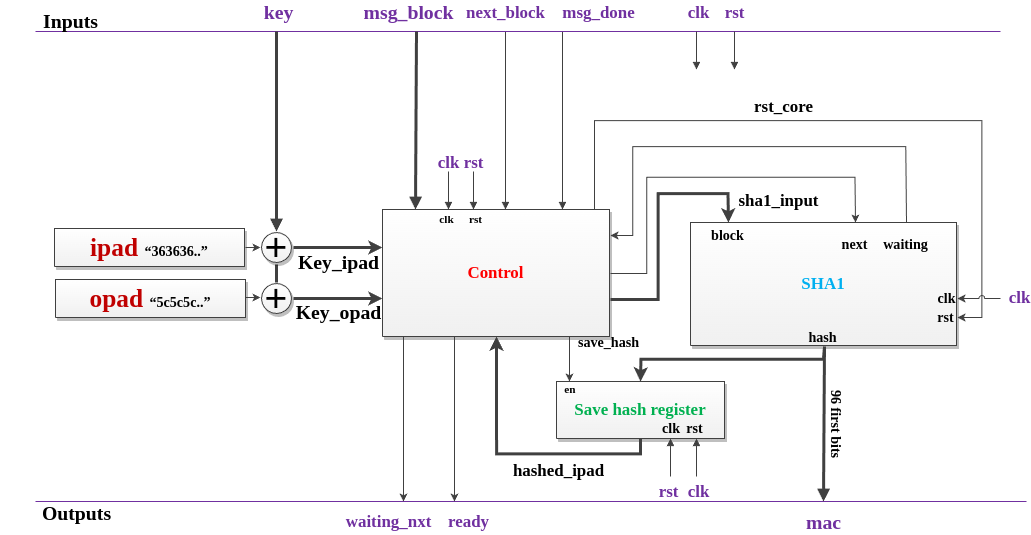
\includegraphics[width= 0.8\textwidth]{figure_5.22}\\
\caption{ hmac\_sha1\_96 module implementation}
\label{fig:figure_5.22}
\end{figure}

The unit consists includes the constants $ipad$ and $opad$, two bitwise XOR operations between these constants and the key, a sha1 unit, a register to store the intermediate calculation of $H((K_0 \oplus ipad) || text)$, and a control unit.

The control unit is responsible for routing the appropriate value to the input of the sha1 unit. This is depicted in Figure \ref{fig:figure_5.22} with the values of $K_0\oplus ipad$, $K_0\oplus opad$, hashed\_ipad, and msg\_block being provided to the control unit. The control unit's FSM is presented in Figure \ref{fig:figure_5.23}.

For each new calculation of HMAC-SHA1-96, the unit is first initialized with a reset signal leading the FSM to the Start state. In this state, the sha1 unit is initialized through a pulse issued on the internal signal rst\_core, while the signal waiting\_nxt is kept active indicating that the unit is ready to accept the first block. Once the first block is provided and the next\_block signal is issued, the FSM transitions to the $Hash(key\oplus ipad)$ state. There the first block of the message $(K_0\oplus ipad) || text$, $(K_0\oplus ipad)$, is routed to the sha1 unit. Once the calculation is completed, the waiting\_next\_block signal of the sha1 unit is issued, and the FSM transitions to the Hash \nth{1} block state, where the first block of the message is given to the sha1 unit. After this calculation finishes, the FSM enters the loop of states Wait Next Block and Hash Next Block. In the Wait Next Block state, the unit waits for the next block, and once provided, it moves to the Hash Next Block state to perform the next calculation on the newly provided block. This process continues until the msg\_done signal is issued, indicating that all blocks of the message have been provided, and therefore, the output of the sha1 unit has the quantity $H((K_0\oplus ipad) || text)$.

When the msg\_done signal is issued, the FSM transitions to the Save Hash state, where the value $H((K_\oplus ipad) || text)$ is stored in the Save Hash Register using the save\_hash signal. In the next clock cycle, the FSM automatically moves to the Reset Core state, where the sha1 unit gets prepared for a new calculation. When the sha1 unit is ready, the calculation $H[(K_0\oplus opad) || H((K_0\oplus ipad) || text)]$ starts. In the $Hash(key\oplus opad)$ state, the block $(K_0\oplus opad)$ is given to the sha1 unit. Once the calculation is finished (i.e., when waiting\_next\_block='1'), the \nth{2} block of the message is provided, $H((K_0\oplus ipad) || text)$. At the end of this calculation, the final MAC value is available at the output of the sha1 unit. The system moves to the Done state, where it issues the ready signal to indicate that the MAC is ready. The first 96 bits of the sha1 result are present at the output of the hmac\_sha1\_96.

% fig 5.23
\begin{figure}
\centering
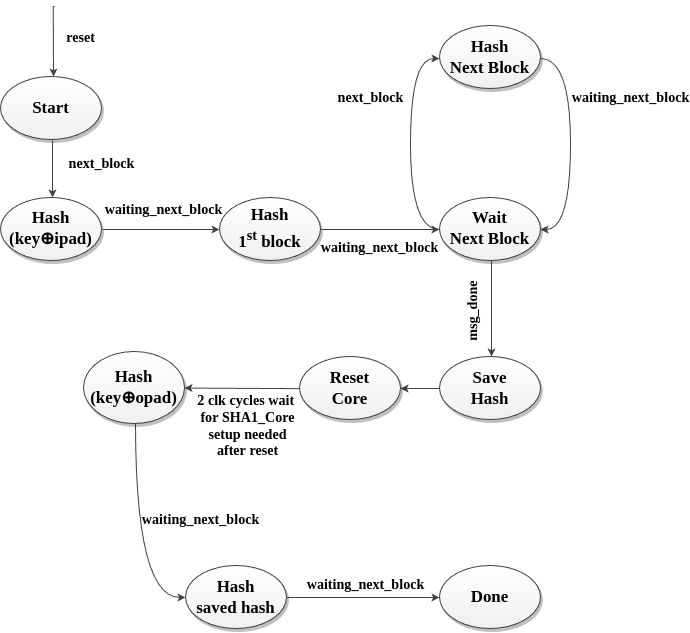
\includegraphics[width= 0.8\textwidth]{figure_5.23}\\
\caption{  hmac\_sha1\_96 control FSM }
\label{fig:figure_5.23}
\end{figure}

\section{Hardware-side Interface}
The interfaces of the two peripheral systems, CBC-AES-128 and HMAC-SHA1-96, are not fully suitable for direct connection to the processor bus. Their inputs and outputs need to be represented with registers corresponding to memory locations of the processor's address space (memory-mapped IO).

Xilinx's toolset offers a procedure for creating and connecting custom-designed peripheral systems. This type of peripheral is referred to by Xilinx as a custom IP core. Through this process, these peripherals and their interfaces are defined. In the case of CBC-AES-128, the interface consists of 17 32-bit registers, of which 4 are used for the input block, 4 for the output block, 4 for the key, 4 for the IV, and the last one serves as a command/status register. The last register, when read by the processor, provides peripheral notification signals, while when written, it sets the peripheral's command signals. It is worth noting that the 4 registers of the output block could overlap with some of the input registers since the former are used only for writing and the latter only for reading. A choice to separate them is made solely to keep the design clear. For HMAC-SHA1-96, there are a total of 36 32-bit registers. 16 are dedicated to the input block, 16 to the key, 3 to its output (a 96-bit MAC), and one is the command/status register. As several bits in the command/status registers remain unused, some signals are exposed through them to assist with the debugging of the peripherals.

\clearemptydoublepage

% Chapter 6
\chapter{Software Components}\label{ch:chap6}
%!TEX root = ../main.tex

\section{lwIP}
lwIP (lightweight IP) (\cite{lwip_docs}, \cite{lwip_wiki}) is an open-source implementation of the TCP/IP stack for embedded systems. Specifically, it implements the Ethernet, ARP, IP, TCP, and UDP protocols. It allows the implementation of user applications with networking requirements on embedded systems.

The most fundamental data structure of lwIP is the p\_buf (packet buffer). p\_buf is used for organizing packets and storing them in memory and is used in all layers of the stack. It contains the headers and data of the packet and additional information such as its size. Along with the p\_buf structure, functions for its processing are provided, such as creation, deletion, extension, etc.

The datapath followed by an incoming packet starts with its reception. Here, the processor is notified through an Ethernet Controller interrupt for the arrival of the new packet. When the processor becomes available, it retrieves the packet from the incoming queue of the Ethernet Controller and creates a new p\_buf for it. Next, the p\_buf is passed upwards from layer to layer. Each layer performs the appropriate processes on the packet, removes its header, and passes it to the next layer. If any layer decides that the packet should be dropped due to failing necessary checks or when it reaches the last processing layer, the p\_buf is deleted an memory is reclaimed. Outgoing packets follow the reverse path.

Each layer offers an interface to other layers. This interface essentially consists of the actions of receiving and transmitting a packet, and some additional layer-specific function. For example, the interface of the IP layer is shown in Listing \ref{lst:ip_interface}.\\

\noindent
\begin{minipage}{\linewidth}
\begin{lstlisting}[style=mycodestyle, label={lst:ip_interface}, caption={IP layer's interface in lwIP}]
struct netif * ip_route(struct ip_addr *dest);

err_t ip_input(struct pbuf *p, struct netif *inp);

err_t ip_output(struct pbuf *p, struct ip_addr *src, struct ip_addr *dest, u8_t ttl, u8_t tos, u8_t proto);

err_t ip_output_if(struct pbuf *p, struct ip_addr *src, struct ip_addr *dest, u8_t ttl, u8_t tos, u8_t proto, struct netif *netif);
\end{lstlisting}
\end{minipage}\\

As observed, the interface consists of input and output functions, and a specialized function of the IP protocol used for routing (ip\_route).
Lastly, each protocol has multiple parameters that can be configured by the designer, such as the TCP timeout, the maximum packet size, etc.

\section{IPsec}
The IPsec implementation is integrated into the existing codebase of lwIP, as mentioned in Chapter ~\ref{ch:4.2.2}. The software development is divided into two parts. The first involves creating in isolation a software library that provides IPsec functionality, and the second involves interfacing and integrating this library with lwIP. The components of the library and their relationships are illustrated in Figure \ref{fig:figure_6.1}. Below, the individual components of the library created for the various IPsec functions and the method of integration with lwIP are explained.


% fig 6.1
\begin{figure}
\centering
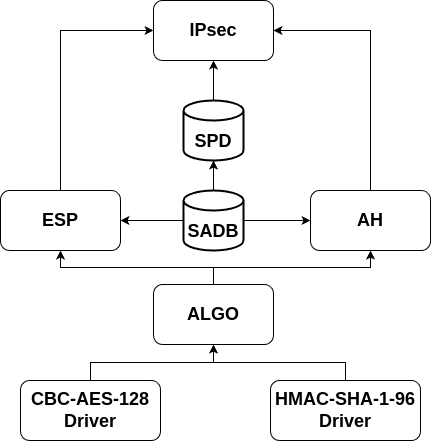
\includegraphics[width= 0.6\textwidth]{figure_6.1}\\
\caption{  Software architecture diagram for the custom IPsec library }
\label{fig:figure_6.1}
\end{figure}

\subsection{IPsec}
The library implementing IPsec provides two functions, one for processing inbound traffic and one for processing outbound traffic. The inbound function is called by the ip\_input of the IP after the packet has been processed by the IP. The outbound function is called at the beginning of the ip\_output\_if  so that every outgoing packet is first processed by IPsec before proceeding. ipsec\_output returns a code to ip\_output\_if so that the latter can select the operations to perform. The function signatures are shown in Listing \ref{lst:ipsec_interface}.\\

\noindent
\begin{minipage}{\linewidth}
\begin{lstlisting}[style=mycodestyle, label={lst:ipsec_interface}, caption={IPsec implemented interface}]
void ipsec_input(struct pbuf *p, struct netif *inp);

u8_t ipsec_output(struct pbuf *p, struct pbuf **p_new, struct ip_addr *src, struct ip_addr *dest, u8_t ttl, u8_t tos, u8_t proto, struct netif *netif);
\end{lstlisting}
\end{minipage}\\

The input function takes the $pbuf$ of the incoming packet and the Ethernet interface where the arrival occurred. Firstly, it extracts the packet fields' values and issues a SADB lookup. If the packet is not matched with any SA, it is discarded. If there is a match, depending on the protocol referenced in the SA, either esp\_input or ah\_input is called. After these functions finish processing the packet and no conditions for packet rejection arise, the SPD is checked to ensure that the packet complies with the policy. If the packet passes the SPD check, it is forwarded to ip\_input as a pure IP packet to continue its path in the TCP/IP stack.

The output function takes the pbuf of the outgoing packet, a pbuf to which the processed packet will be assigned as a result of ipsec\_output, the IP addresses of the sender and receiver, the TTL and TOS values of the packet, and the Ethernet interface that will perform the transmission. The function returns a code, whose values correspond to:

\begin{outline}
\1 RET\_IPSEC\_ERROR if an errors occur,
\1 RET\_IPSEC\_BYPASS for applying the BYPASS policy,
\1 RET\_IPSEC\_APPLY for applying the PROTECT policy,
\1 RET\_IPSEC\_DISCARD for applying the DISCARD policy.
\end{outline}

The ipsec\_output initially searches the SPD. If no policy is found, the packet is discarded. If found, if it's a DISCARD policy, the function simply returns the RET\_IPSEC\_DISCARD code. If it's BYPASS traffic, no processing is performed on the packet, and the function returns with the RET\_IPSEC\_BYPASS code. If it's PROTECT traffic, depending on the protocol defined in the policy's SA, the packet is passed to either ah\_output or esp\_output. If they return without errors, the function returns with the RET\_IPSEC\_APPLY code; otherwise, with the RET\_IPSEC\_ERROR code. If an error occurs at any point in ipsec\_output, it returns with the RET\_IPSEC\_ERROR code.

The ipsec\_output returns to ip\_output\_if, which has been modified to interpret the return value of ipsec\_output properly. Thus, when RET\_IPSEC\_ERROR is returned, it discards the packet and reports an error. When RET\_IPSEC\_BYPASS is returned, the regular IP processing is executed. If RET\_IPSEC\_APPLY is returned, the packet is a ready IP packet for transmission due to processing by ah\_output or esp\_output and is sent without further processing. Finally, if RET\_IPSEC\_DISCARD is returned, ip\_output\_if discards the packet and releases the memory.



\subsection{AH and ESP}
The main processing of packets in IPsec is performed by the AH and ESP protocols. These protocols add additional headers and populate the header fields. Packets undergo cryptographic transformations for outgoing traffic, while header fields are checked and packets undergo reverse cryptographic transformations and checks for incoming traffic.

For incoming traffic, the implementation of AH and ESP provide an input function, ah\_input and esp\_input respectively. These functions are called by ipsec\_input, with arguments being the pbuf of the packet and the corresponding SA. Both functions start by checking the Sequence Number. Then the authentication and integrity checks follow which are mandatory for AH but optional for ESP. Next, for ESP only, the packet gets decrypted. The parameters for all these operations are found in the applicable SA. Finally, both functions consult the SA regarding the IPsec mode in which they should process the packet. In the case of Transport Mode, the IPsec header is removed, and the IP header is prepended to the payload. For Tunnel Mode, the outer header and the IPsec header are removed, leaving the inner header intact. A the end of these processes, we obtain an IP packet which is forwarded to ip\_input accordingly. The interfaces for AH and ESP inbound process are shown in Listing \ref{lst:ah_esp_in_interface}.\\

\noindent
\begin{minipage}{\linewidth}
\begin{lstlisting}[style=mycodestyle, label={lst:ah_esp_in_interface}, caption={AH and ESP inbound processing  interfaces}]
int ah_input(struct pbuf* p, struct sa_entry* sa);
int esp_input(struct pbuf* p, struct sa_entry* sa);
\end{lstlisting}
\end{minipage}

For outbound traffic, the functions ah\_output and esp\_output are provided, which are called by ipsec\_output. Their arguments include the pbuf of the packet, a new pbuf where the processed packet will be placed, the policy entry found by ipsec\_output, as well as the IP addresses of the sender and recipient, the values of TTL and TOS, and the interface from which the packet will be sent. TTL and TOS are provided by the Transport Layer protocols and are given to ah\_output and esp\_output so that they can construct the inner IP header and, if it is tunnel mode traffic, the outer IP header too. The interfaces for AH and ESP inbound process are shown in Listing \ref{lst:ah_esp_out_interface}.\\

\noindent
\begin{minipage}[t]{\linewidth}
\begin{lstlisting}[style=mycodestyle, label={lst:ah_esp_out_interface}, caption={AH and ESP outbound  processing interfaces}]
err_t ah_output(struct pbuf *p, struct pbuf **p_new, struct spd_entry* spdentry, struct ip_addr *src, struct ip_addr *dest, u8_t ttl, u8_t tos, u8_t proto, struct netif *netif);

err_t esp_output(struct pbuf *p, struct pbuf **p_new, struct spd_entry* spdentry, struct ip_addr *src, struct ip_addr *dest, u8_t ttl, u8_t tos, u8_t proto, struct netif *netif);
\end{lstlisting}
\end{minipage}

Packet processing begins with the placement of the inner IP header if in Tunnel Mode. Then, for ah\_output, the AH header is placed, followed by the outer IP header, and finally, the packet goes through the integrity and authentication algorithm, and the ICV value is placed in the appropriate field before being handed back to ipsec\_output.

In esp\_output, after the possible placement of the inner IP header, padding and IV are added, followed by encrypting all of the above together with the payload. Then, the ESP header is added, and if integrity is used, the integrity algorithm is applied. The ICV of the integrity algorithm is placed at the end of the packet, and finally, the outer IP header is added. Upon returning from esp\_output to ipsec\_output, the processed packet is ready to continue its transmission.


\subsection{SADB and SPD}
The SADB is implemented as a unidirectional linked list. Each entry in the SADB represents an SA. The structure implemented to represent an SA contains:

\begin{outline}
\1 the SPI number
\1 the IANA number of the protocol
\1 the mode corresponding to the traffic (transport or tunnel)
\1 the packet sequence number (Sequence Number)
\1 The authentication algorithm used by AH (if applicable, i.e., if AH protocol \1 is used for this traffic)
\1 If applicable, the key is also retained.
\1 The authentication algorithm used by ESP (if applicable, i.e., if ESP \1 protocol is used and authentication is used for this traffic simultaneously)
\1 If applicable, the key is also retained.
\1 The encryption algorithm of ESP (mandatory if ESP is used).
\1 If applicable, the key is also retained.
\1 A pointer to the next SADB entry to maintain a unidirectional linked list.
\end{outline}

\noindent
The definition of the structure is shown in Listing \ref{lst:sadb}.\\

\noindent
\begin{minipage}{\linewidth}
\begin{lstlisting}[style=mycodestyle, label={lst:sadb}, caption={The SADB entry structure}]
struct sa_entry
{
	u32_t spi;
	u8_t protocol;	
	u8_t mode;		// Transport or Tunnel
	
	/* Current Connection */
	u32_t seqnum; 
	
	/* Algorithms */
	struct auth_algo* ah_auth_algo;
	u8_t* ah_auth_key;
	
	struct enc_algo* esp_enc_algo;
	u8_t* esp_enc_key;
	
	struct auth_algo* esp_integrity_algo;
	u8_t* esp_integrity_key;
	
	/* Linked entries*/
	struct sa_entry *next;

}__attribute__((packed));
\end{lstlisting}
\end{minipage}\\

The structures auth\_algo and enc\_algo are created to add a flexible interface for cryptographic algorithm integration. They serve as an intermediate layer between IPsec and the algorithm interfaces. If a new cryptographic algorithm needs to be used, it is sufficient to create an auth\_algo or enc\_algo structure (depending on the type of algorithm) so that it can be directly utilized by the specific IPsec implementation.

The SADB library provides functions for creating and adding a new SA to the database and for searching for an SA based on the SPI and protocol number values. The search function returns the entry if found. The signatures of these functions are shown in Listing \ref{lst:sadb_interface}.\\

\noindent
\begin{minipage}{\linewidth}
\begin{lstlisting}[style=mycodestyle, label={lst:sadb_interface}, caption={The SADB interface}]
struct sa_entry *sa_lookup(u32_t spi, u8_t proto);

struct sa_entry* sa_add(u32_t spi, u8_t protocol, u8_t mode, 
				  struct auth_algo* ah_auth_algo, u8_t* ah_auth_key,
				  struct enc_algo* esp_enc_algo, u8_t* esp_enc_key,
				  struct auth_algo* esp_integrity_algo, u8_t* esp_integrity_key);
\end{lstlisting}
\end{minipage}\\

Similarly to SADB, SPD is implemented as a unidirectional linked list. Each entry in the list represents a policy and includes:
\begin{outline}
    \1 The sender's IP address
    \1 The sender's subnet mask
    \1 The receiver's IP address
    \1 The receiver's subnet mask
    \1 The protocol's IANA number
    \1 The type of policy (PROTECT, BYPASS, DISCARD)
    \1 The direction of traffic (IN or OUT)
    \1 The IPsec protocol used in the case of the PROTECT policy (AH or ESP)
    \1 The mode (Transport or Tunnel)
    \1 The sender's IP address of the tunnel
    \1 The receiver's IP address of the tunnel
    \1 The SA that characterizes the policy's traffic
    \1 A pointer to the next entry in the SPD to implement the unidirectional linked list.
\end{outline}

\noindent
The definition of the structure is shown in Listing \ref{lst:spd_entry}.\\

\noindent
\begin{minipage}{\linewidth}
\begin{lstlisting}[style=mycodestyle, label={lst:spd_entry}, caption={The SPD entry strucutre}]
struct spd_entry{

	struct 
	ip_addr*	src ;			/**< IP source address */
	u32_t  		src_netaddr ;		/**< net mask for source address */
	struct 
	ip_addr*	dest ;			/**< IP destination address */
	u32_t		dest_netaddr ;		/**< net mask for the destination address */
	u8_t		protocol ;		/**< the transport layer protocol */
	u8_t		policy ;			/**< defines how this packet must be processed*/
	u8_t		direction;		/**< defines IN or OUT traffic direction */
	u8_t		ipsec_proto;		/**< AH or ESP processing */
	u8_t		ipsec_mode;		/**< Transport or Tunnel mode */
	struct 
	ip_addr*	tunnel_src;		/**< IP tunnel source */
	struct 
	ip_addr *	tunnel_dest;		/**< IP tunnel destination */
	
	struct
	sa_entry*	sa ;			/**< pointer to the associated SA */
	struct
	spd_entry*	next ;			/**< pointer to the next table entry*/
}
\end{lstlisting}
\end{minipage}\\

The SPD library provides functions for creating and adding a new policy to the database, as well as for searching for a policy based on the sender's and receiver's IP and subnet mask values and the protocol number. The search function returns the entry if found. The signatures of these functions is shown in Listing \ref{lst:spd_interface}.\\

\noindent
\begin{minipage}{\linewidth}
\begin{lstlisting}[style=mycodestyle, label={lst:spd_interface}, caption={The SPD interface}]
struct spd_entry* spd_lookup(struct ip_addr *src, u32_t src_netaddr, 
struct ip_addr *dest, u32_t dest_netaddr, u8_t proto);
	
void spd_add(struct ip_addr *src, struct ip_addr *dest, u8_t proto, 
    u8_t policy, u8_t direction, u8_t ipsec_proto, u8_t ipsec_mode,
    struct ip_addr *tunnel_src, struct ip_addr *tunnel_dest,
    struct sa_entry* sa);
\end{lstlisting}
\end{minipage}\\


\section{Integration with lwIP}
The software interface of the implemented IPsec library consists of two functions, one for processing incoming packets and one for processing outgoing packets.

The modifications in lwIP are made at the IP level since IPsec belongs to this layer. For inbound traffic, the packet must pass through IPsec after being processed by IP. Thus, the ip\_input function is modified to hand over control to the IPsec input routine. Specifically, ip\_input first processes the packet, and when finished, decides which protocol to pass the packet's payload to. Here, the option of IPsec for AH and ESP protocols is introduced. Figure \ref{fig:figure_6.2} illustrates the flowchart before and after modification of the inbound processing.

% fig 6.2
\begin{figure}
\centering
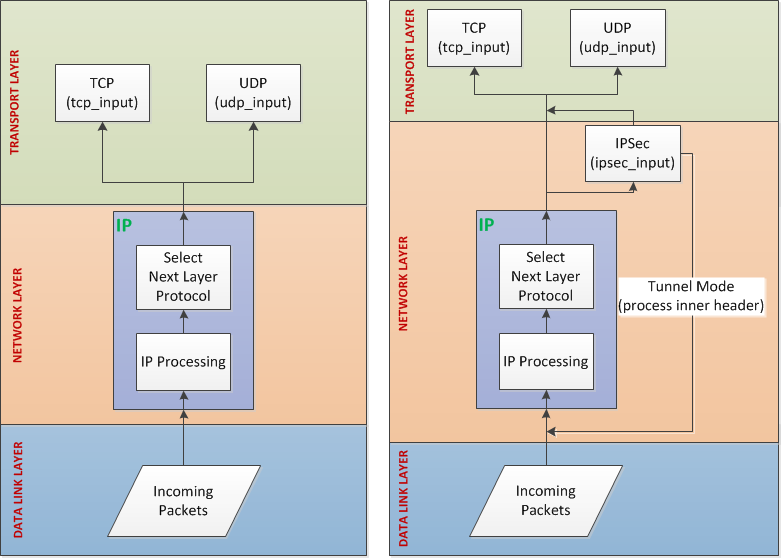
\includegraphics[width= 0.8\textwidth]{figure_6.2}\\
\caption{  Integration of inbound IPSec packet processing in lwIP }
\label{fig:figure_6.2}
\end{figure}

The function ipsec\_input serves as the interface for incoming IPsec packets. If the next hop after IP is IPsec, then the packet is handed over via ipsec\_input. At the end of IPsec processing, if the packet is in Transport Mode, it is forwarded to the appropriate Transport Layer protocol. If the packet is in Tunnel Mode, then it is passed back to the IP layer for further processing of the inner IP header and subsequently forwarded to one of the Transport Layer protocols.

For outbound traffic, the packet must first be passed to IPsec, and if it passes all the checks, it is handed over to IP for transmission. In this case, changes are made to the ip\_output\_if function. This is more heavily modified compared to ip\_input, as a considerable amount of IPsec code had to be executed before transferring the packet to the IP layer, such as searching the SPD and creating the IPsec header.

% fig 6.3
\begin{figure}
\centering
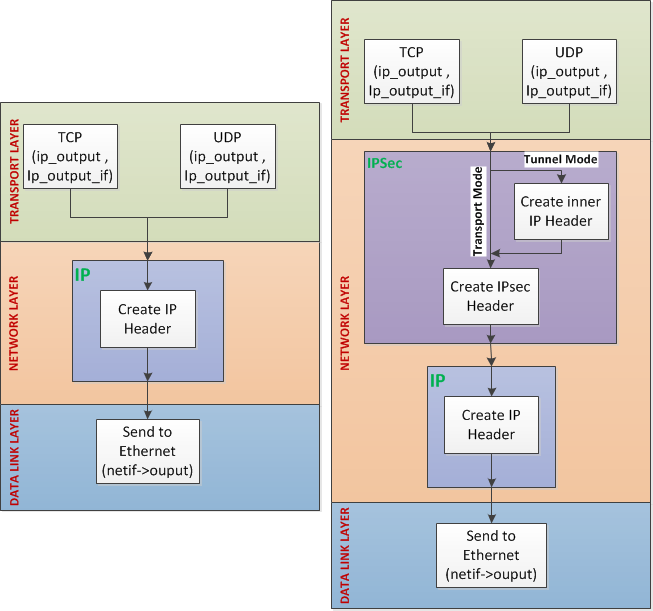
\includegraphics[width= 0.8\textwidth]{figure_6.3}\\
\caption{  Integration of outbound IPSec packet processing in lwIP }
\label{fig:figure_6.3}
\end{figure}

The flowcharts for outbound traffic of lwIP and modified lwIP are shown in Figure \ref{fig:figure_6.3}. When a packet is forwarded from one of the transport layer protocols to IP, the ip\_output or ip\_output\_if function is invoked. During execution in the modified lwIP, the packet is first processed by IPsec and then by IP. In processing by IPsec, we have two cases: the first is when the packet belongs to tunnel mode traffic, where the inner IP header is placed first, followed by the IPsec header, and the second is when we are in transport mode traffic, so only the IPsec header is placed.


\section{Software-side Interface}
Software drivers are created for the two peripherals to abstract out the details of handling the hardware interface from the rest of the software. Specifically, these drivers handle the movement of data between memory and peripherals and utilize the communication protocol of the peripheral to control its operation. They provide certain functions to the system to seamlessly execute cryptographic operations using the peripherals.

For the CBC-AES-128 peripheral, the driver has two functions, one for encrypting and one for decrypting a message. Their inputs are the memory location from which the message starts, the size of the message, the memory location from which the key starts, and the memory location from which the IV starts. Initially, the key, IV, and the first block of the message are copied from memory to the appropriate registers of the peripheral. Then, a start\_new signal is issued along with a suitable value of the EncDec signal ('0' for encryption, '1' for decryption) to notify the peripheral that a computation on a new message is starting. The driver then waits for the peripheral's ready signal to be issued. Once issued, it copies the result to the memory locations where the original block was, copies the next block, and issues a next\_block signal. It then waits again for the ready signal, then copies the result to memory, and then issues the next block. This process repeats until all input blocks are processed. It is noted here that using CBC-AES-128 with ESP relieves the driver from performing padding, as the packet already contains padding from ESP processing. The function signatures and their operation are described using pseudocode in Listing \ref{lst:aes_driver}. \\


\begin{lstlisting}[style=mycodestyle, label={lst:aes_driver}, caption={AES driver pseudocode}]
void AES128_CBC_encrypt(void* data, u32_t length,  void* key, void* iv)
{
	Copy the first 128 bits of data to the peripheral
	Copy key to the peripheral
	Copy iv to the peripheral

	Send start_new=’1’ and EncDec = ‘0’
	Wait until ready=’1’
	Copy result in the first 128 bits of data

        For all the next 128 bits blocks of data:
	   Copy the next 128 bits of data
	   Send next_block
	   Wait until ready=’1’
	   Copy result in the corresponding 128 bits of data
}

void AES128_CBC_decrypt(void* data, u32_t length, void* key, void* iv)
{
	Copy the first 128 bits of data to the peripheral
	Copy key to the peripheral
	Copy iv to the peripheral

	Send start_new=’1’ and EncDec = ‘1’
	Wait until ready=’1’
	Copy result in the first 128 bits of data

        For all the next 128 bits blocks of data:
	   Copy the next 128 bits of data
	   Send next_block
	   Wait until ready=’1’
	   Copy result in the corresponding 128 bits of data
}
\end{lstlisting}\\

For the peripheral HMAC-SHA1-96, the driver provides two functions, one for generating the MAC of a message and one for comparing a given MAC with the MAC of a message. Both functions execute the hmac-sha1-96 on the message, and their only difference is that the first one copies the MAC result to a specific memory area, while the second one compares the MAC result with another MAC and returns the comparison result. The former is used by IPsec to create the MAC of a new packet and place it in the appropriate field, while the latter is used to authenticate an incoming packet.

The procedure for handling the HMAC-SHA1-96 peripheral is as follows: initially, for each new message (packet), a reset signal is provided. Then, the driver copies the key and the first block of the message from memory to the appropriate registers of the peripheral and issues a next\_block signal. Subsequently, the driver waits for the waiting\_nxt signal to place the next block and issues the next\_block signal again. This process continues for all blocks, and once all the message blocks are processed, a msg\_done signal is issued, and the driver is then waiting for the ready signal. Finally, once the ready signal is issued, if we are in the MAC generation function, the result is copied to memory, while if we are in the comparison function, the result is compared with the given MAC, and the comparison result is returned. It is noted that the padding of the block is calculated in the driver functions and that the key size is exactly 160 bits, so no preprocessing is needed.
Below are the function signatures and their operation described using pseudocode in Listing \ref{lst:hmac_driver}.\\

\begin{lstlisting}[style=mycodestyle, label={lst:hmac_driver}, caption={HMAC driver pseudocode}]
int HMAC_SHA1_96_authenticate(void* data, u32_t datalength, void* key, 
    u32_t keylength, void* icv)
{
    Padding execution,
    Send rst
    
    For each block of 512 bits of the message:
        Copy the first 512 bits of the message
        Send next_block='1'
        Wait for waiting_nxt
        Send msg_done
        Wait for ready='1'

        If icv == result of the peripheral
            Return 1
        Else
            Return 0
}

void HMAC_SHA1_96_calculate(void* data, u32_t datalength, void* key, u32_t keylength, 
                    void* icv)
{
    Padding execution,
    Send rst
    
    For each block of 512 bits of the message:
        Copy the first 512 bits of the message
        Send next_block='1'
        Wait for waiting_nxt
        Send msg_done
        Wait for ready='1'
        Copy the result of the peripheral to icv
}

\end{lstlisting}
\clearemptydoublepage

% Chapter 7
\chapter{FPGA Implementation and On-Chip Verification}\label{ch:chap7}
%!TEX root = ../main.tex

\section{Tools}
\subsection{Xilinx Suite and Modelsim}
For the designing process, the Microblaze programming, the custom IP cores implementation, and the board programming, the Xilinx tool suite, Xilinx ISE Design Suite 13.1 \cite{xilinx_ise_13_1}, is utilized. For simulating the design, Modelsim is preferred due to its capabilities and direct integration with Xilinx tools.

ISE comprises tools for hardware synthesis in VHDL or Verilog. It provides syntax checking, direct simulation, and hardware synthesis for FPGA programming. This toolset is used for the implementation of the cryptographic algorithms.

An important tool within ISE is the Embedded Development Kit (EDK), which aids in system design, offering an easy instantiation of different processors and a plethora of ready-to-use peripherals. It supports configuration options of several system parameters, such as processor cache size, peripheral addressing schemes, different bus types instantiations, and choice amongst several interfacing options between processors and peripherals. Additionally, custom IP Cores can be easily integrated into the system using EDK. The IPsec system is defined using EDK, the Ethernet, UART, and DDR2 peripherals are added, and the custom cryptographic IP cores AES-128 and HMAC-SHA1-96 are integrated.

Another crucial tool is the Software Development Kit (SDK). It helps manage the system's software, from implementing a simple routine to loading a full-fledged operating system onto processors (e.g., Xilkernel or embedded Linux). It supports programming in C, C++, and assembly. Moreover, it offers ready-to-use software systems such as the lwIP protocol stack and the Xilkernel operating system. From this tool, the software can be downloaded and run in an FPGA system. Software debugging is also performed using SDK. Finally, it includes monitoring of a serial port, allowing us to receive program messages through STDIO (standard input-output). The IPsec code is developed and integrated into the lwIP library using this tool.

Modelsim is a widely used hardware simulator program. It is directly integrated into ISE, which eliminates the need to manually include Xilinx libraries in Modelsim. Furthermore, it provides automation capabilities for simulation, based on the Tcl language, boosting productivity during design 
 debugging and verification. Tcl is used during the CBC-AES-128 verification, in order to automatically simulate and verify the design's correctness against the FIPS test vectors.

\subsection{Wireshark}
Wireshark \cite{wireshark_wiki} is one of the most famous traffic analyzers. Its primary function is to monitor a network interface (e.g., Ethernet, Wi-Fi, etc.) and display the packets moving through it. It is extensively used during the IPsec implementation and testing phase to aid in software debugging.

Wireshark conveniently presents packets, recognizing a vast range of protocols and displaying all fields of each protocol in a structured manner. Additionally, packets can be displayed in their "raw" form, i.e., in binary or hexadecimal representation, a feature that is particularly helpful in the debugging of cryptographic algorithms. For the AH and ESP protocols, it provides automatic integrity checking and decryption if the specific SA is provided. Lastly, it offers traffic filtering with a wide range of options which is useful for displaying only packets of interest and avoiding a noisy display of all packets present in real networks.

\subsection{Scapy}
Scapy \cite{Scapy_documentation} is a tool based on the Python programming language. It provides a command language for creating packets of any layer of the stack. It can also send the crafted packet and receive and report responses to them. With Scapy, both predefined packets such as IP, TCP, UDP, etc., can be created as well as packets from their hexadecimal form (Raw).

Scapy is used for debugging and verification of the system's inbound dataflow. By connecting a PC to the FPGA, we can create and send individually crafted packets targeting specific behaviors of the input code of IPsec.

\subsection{Linux ipsec-tools}
The ipsec-tools is the implementation of IPsec for the Linux operating system. It allows us to define SPs and SAs either manually or using IKE.

ipsec-tools is used in the final phase of the implementation as a reference system for the final verification stage. Specifically, ipsec-tools is installed on a computer which is connected to the FPGA. Then, SPs and SAs are defined manually on both the computer and the FPGA. Theis setup allows for verification of the implementation against a real-world system running IPsec.

One might notice that using Scapy in debugging is redundant since ipsec-tools can replace its functionality. The power of Scapy comes from allowing segmented testing, providing fine-grained access to every packet detail, whereas ipsec-tools would require significant effort in additional development to achieve the same. 

\section{Final System Design and Implementation}
Figure \ref{fig:figure_7.1} depicts the high-level diagram of the complete system. The diagram distinguishes which parts are implemented on the FPGA chip and which are located on the board. Microblaze, its peripherals, and a local memory are situated within the FPGA chip. Microblaze is connected to its peripherals via a PLB bus. All peripherals are memory-mapped. The interfaces of the CBC-AES-128 and HMAC-SHA1-96 peripherals are also presented, detailing their registers.

The FPGA chip, external RAM, the serial port (UART) interface and the Ethernet interface are located on the board.

Received incoming packets are placed in a FIFO by the Ethernet interface. The next available packet in FIFO is moved from the Ethernet interface to the Ethernet Controller when the latter is ready. The Ethernet Controller then notifies the Microblaze via an interrupt. The Microblaze interrupts its operation and executes the lwIP Ethernet code responsible for incoming packets, which stores the new packet in RAM, processes the Ethernet packet, and then passes the execution control to the protocol encapsulating the Ethernet packet. In the case of an IP packet, ip\_input is executed next. In the case of an IPsec packet, the payload of the IP packet is passed to ipsec\_input, which checks the SPD and SADB databases, distinguishes between AH or ESP packets, and executes the appropriate function. When it reaches the point of authentication and/or decryption, the execution control proceeds to the corresponding driver. The driver copies blocks of the payload from RAM to the peripheral, issues the appropriate commands, waits for a response from the peripheral, and finally copies the result back to RAM. Once IPsec processing is completed, the payload of the IPsec packet is passed to the appropriate higher-layer protocol. The process of processing outgoing packets follows the reverse flow, starting from a higher-layer packet and ending in the output FIFO and finally transmission via the Ethernet interface. Lastly, during IPsec execution, debugging messages are generated and sent through the UART interface to a PC.

% fig 7.1
\begin{figure}
\centering
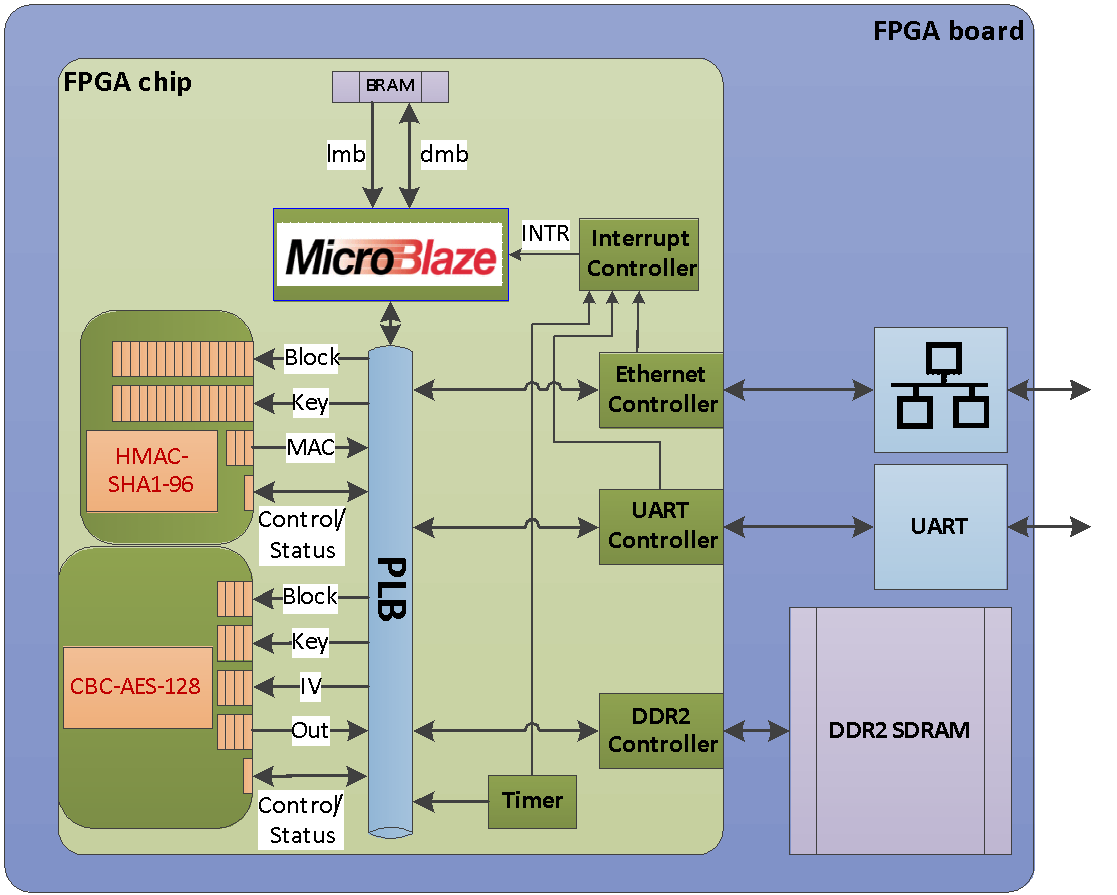
\includegraphics[width= 0.8\textwidth]{figure_7.1}\\
\caption{ Complete system architecture. }
\label{fig:figure_7.1}
\end{figure}

\section{On-Chip Verification}
An ECHO server is implemented for testing the system's operation in a near-real application scenario. The ECHO server accepts requests that carry a message and responds to the requester, echoing back the same message. The server is deployed on the FPGA. The setup is shown in Figure \ref{fig:figure_7.2}. 

A Ruby script served as a client of the ECHO server. It establishes a connection with the server and then sends ECHO requests. The code snippet shown in Listing \ref{lst:echo_client}, serves as an example of a client. It connects to the ECHO server and then sends 1000 randomly sized messages with a payload ranging from 5 to 50 random uppercase characters. If a disparity between the request and response arises, the transmission halts and the fault is reported. Finally, the connection is closed.\\

\noindent
\begin{minipage}{\linewidth}
\begin{lstlisting}[style=mycodestyle, label={lst:echo_client}, caption={ECHO client Ruby implementation}]
require ‘socket’
cl=TCPSocket.new(Server_IP, 7)
for i in 0..1000
 	    random_message = (0..(rand(50)+5).map{ (65+rand(26)).chr }.join
    cl.puts random_message
    if cl.gets != random_message then
        puts “Unexpected Response”
        break
    end
end
cl.close  
\end{lstlisting}
\end{minipage}\\

% fig 7.2
\begin{figure}
\centering
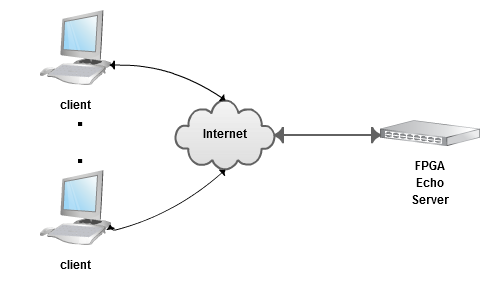
\includegraphics[width= 0.8\textwidth]{figure_7.2}\\
\caption{ ECHO server in Transport Mode }
\label{fig:figure_7.2}
\end{figure}

The preparation of the setup includes configuring the policies in the SPD and the SAs in the SADB \cite{setkey_manpage} of both systems and setting up Wireshark for collecting the relevant packets. The system is tested for both protocols (AH and ESP) using a large number of packets. As an example, the packets of one request-response scenario are presented in Figures \ref{fig:figure_7.3}, \ref{fig:figure_7.4}, \ref{fig:figure_7.5},  \ref{fig:figure_7.6}, \ref{fig:figure_7.7} and \ref{fig:figure_7.8}.

\subsubsection*{ESP with CBC-AES-128 and HMAC-SHA1-96 in Transport Mode}

Initially, an ECHO Request with the message "abc" is sent from the client to the server located on the FPGA. The encrypted ESP packet is presented in Figure \ref{fig:figure_7.3}. The colored fields are, in order of appearance:
\begin{outline}
    \1 Ethernet Header
    \1 IP Header
    \1 SPI
    \1 Sequence Number
    \1 IV
    \1 Payload
    \1 ICV
\end{outline}

Figure \ref{fig:figure_7.4} depicts the decrypted payload. The first field is the TCP packet, which, as indicated in the ASCII view, contains the "abc" message. The padding, pad length, and next header follow as part of the second field. The last field is the ICV.

% fig wireshark 1
\begin{figure}[H]
\centering
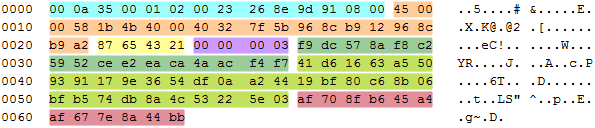
\includegraphics[width= 0.8\textwidth]{figure_7.3}\\
\caption{ Transmitted packet of ECHO request in ESP Transport Mode  }
\label{fig:figure_7.3}
\end{figure}

Next, the ECHO server on the FPGA responds. The response is shown in Figure \ref{fig:figure_7.5}.

% fig wireshark 2
\begin{figure}[H]
\centering
\includegraphics[width= 0.8\textwidth]{figure_7.4}\\
\caption{ Decrypted payload of the ECHO request in ESP Transport Mode }
\label{fig:figure_7.4}
\end{figure}

We observe the presence of the SPI, Sequence Number, IV fields, the encrypted payload, and the ICV. The decrypted packet of the response is shown in Figure \ref{fig:figure_7.6}.

% fig wireshark 3
\begin{figure}[H]
\centering
\includegraphics[width= 0.8\textwidth]{figure_7.5}\\
\caption{ ECHO server response in ESP Transport Mode }
\label{fig:figure_7.5}
\end{figure}

We observe that the original message of the request, 'abc', exists in the decrypted payload.

\subsubsection*{AH with HMAC-SHA1-96 in Transport Mode}
Initially, an ECHO Request with the message "abc" is sent from the client to the server located on the FPGA. The AH packet is presented in Figure \ref{fig:figure_7.7}. The colored fields are in the order of appearance:

\begin{outline}
    \1 Ethernet Header
    \1 IP Header
    \1 Next Header
    \1 AH Length
    \1 Reserved
    \1 SPI
    \1 Sequence Number
    \1 ICV
    \1 TCP Payload
    \1 ECHO Payload    
\end{outline}


% fig wireshark 4
\begin{figure}[H]
\centering
\includegraphics[width= 0.8\textwidth]{figure_7.6}\\
\caption{ Decrypted payload of ECHO server response in ESP Transport Mode }
\label{fig:figure_7.6}
\end{figure}

% fig wireshark 5
\begin{figure}[H]
\centering
\includegraphics[width= 0.8\textwidth]{figure_7.7}\\
\caption{ Transmitted packet of ECHO request in AH Transport Mode }
\label{fig:figure_7.7}
\end{figure}

\begin{figure}[H]
\centering
\includegraphics[width= 0.8\textwidth]{figure_7.8}\\
\caption{ ECHO server response in AH Transport Mode}
\label{fig:figure_7.8}
\end{figure}

\noindent
The FPGA's response is shown in Figure \ref{fig:figure_7.8}.
We observe the presence of the fields in the AH header, as well as the correct content in the ECHO payload.

\section{Evaluation}
Data collection of performance metrics is performed. The purpose of these measurements is to estimate the system's performance and calculate the efficiency gains that the hardware cryptographic algorithms offer compared to a software-only implementation. The metric measured is the number of clock cycles required for processing a packet from the moment it enters the processing path we want to measure. An on-chip timer is used for counting clock cycles. When IPsec processing begins, the timer is initialized and activated. Upon activation, the timer increments its counter value by one at each clock cycle. To measure the processing time of a particular path, we store the timer value at the beginning and end. Subtracting these two quantities yields the number of clock cycles that the specific execution path took.

For comparison with a software-only implementation, the same system is modified using software cryptographic algorithms. The algorithms are implemented based on the OpenSSL package, with minor modifications for porting the code to our system. This decision is made because the implementation of the algorithms in OpenSSL is highly optimized and thus it provides a competitive comparison.

The measurements were conducted using the ESP protocol since it uses both cryptographic algorithms. The measurements are divided into two parts, one for the processing of incoming packets and one for the processing of outgoing ones. Additionally, various payload sizes are used to provide a complete performance picture, as there are parts of the system whose processing time is dependent on the packet size. The paths measured include the total processing of IPsec, the ESP processing, and both of the cryptographic algorithms. It should be noted that the measurement of IPsec includes ESP processing, and ESP includes the cryptographic algorithms execution. The measurements are presented in Table \ref{table:7.1} for inbound traffic and in Table \ref{table:7.2} for outbound traffic. The quantities are expressed in the number of clock cycles.

The tables include a row labeled 'Speedup,' indicating how many times faster the hardware implementation of the measured part is compared to the software implementation. This calculation is the division of the number of clock cycles of the software implementation by those of the hardware implementation. Two additional columns are added for the processing time of only the ESP header (i.e., without the cryptographic algorithms) and for the processing time of the IPsec without ESP processing (i.e., including the IPsec header processing and searches in the SPD and SADB).

% table 7.1
% Please add the following required packages to your document preamble:
% \usepackage{multirow}
% \usepackage[table,xcdraw]{xcolor}
% Beamer presentation requires \usepackage{colortbl} instead of \usepackage[table,xcdraw]{xcolor}
\begin{table}[]
\centering
\begin{tabular}{llllllll}
\toprule
% \multicolumn{8}{|c|}{\textbf{Inbound packet processing}} \\
% \hline
\textbf{\begin{tabular}[|c|]{@{}l@{}}Payload\\ size\\ (bytes)\end{tabular}} &    &     &     &   &   & \textbf{\begin{tabular}[c]{@{}l@{}}ESP \\ Header\\  Processing\end{tabular}} & \textbf{\begin{tabular}[c]{@{}l@{}}IPsec \\ Header\\  Processing\end{tabular}} \\
      & \multirow{-3}{*}{\textbf{HW/SW}} & \multirow{-3}{*}{\textbf{AES}} & \multirow{-3}{*}{\textbf{HMAC}} & \multirow{-3}{*}{\textbf{ESP}}  & \multirow{-3}{*}{\textbf{IPsec}}   &  & \\
      \hline
      & SW	 & 772693	 & 279229	 & 1054804	 & 1057353 & 2882       & 2549 \\
      & HW    & 17625     & 49741     & 70174   & 72724   & 2808       & 2550 \\
\multirow{-3}{*}{\textbf{3}}     & {\color[HTML]{00B050} \textbf{Speedup}}   & {\color[HTML]{00B050} \textbf{43.84}}   & {\color[HTML]{00B050} \textbf{5.61}} & {\color[HTML]{00B050} \textbf{15.03}} & {\color[HTML]{00B050} \textbf{14.54}} & -       & - \\
\midrule
      & SW    & 771658    & 279396    & 1053938    & 1056474    & 2884       & 2536 \\
      & HW    & 17598     & 49697     & 70104   & 72640   & 2809       & 2536 \\
\multirow{-3}{*}{10}    & {\color[HTML]{00B050} \textbf{Speedup}}   & {\color[HTML]{00B050} \textbf{43.85}}   & {\color[HTML]{00B050} \textbf{5.62}} & {\color[HTML]{00B050} \textbf{15.03}} & {\color[HTML]{00B050} \textbf{14.54}} & -       & - \\
\midrule
      & SW    & 3062302   & 316804    & 3381984    & 3384517    & 2878       & 2533 \\
      & HW    & 59600     & 63569     & 125973  & 128503  & 2804       & 2530 \\
\multirow{-3}{*}{100}      & {\color[HTML]{00B050} \textbf{Speedup}}   & {\color[HTML]{00B050} \textbf{51.38}}   & {\color[HTML]{00B050} \textbf{4.98}} & {\color[HTML]{00B050} \textbf{26.85}} & {\color[HTML]{00B050} \textbf{26.34}} & -       & - \\
\midrule
      & SW    & 12619006     & 589613    & 13211500   & 13214036   & 2881       & 2536 \\
      & HW    & 234658    & 132484    & 369958  & 372492  & 2816       & 2534 \\
\multirow{-3}{*}{500}      & {\color[HTML]{00B050} \textbf{Speedup}}   & {\color[HTML]{00B050} \textbf{53.78}}   & {\color[HTML]{00B050} \textbf{4.45}} & {\color[HTML]{00B050} \textbf{35.71}} & {\color[HTML]{00B050} \textbf{35.47}} & -       & - \\
\midrule
      & SW    & 24467280     & 947749    & 25417904   & 25420434   & 2875       & 2530 \\
      & HW    & 451749    & 226794    & 681356  & 683890  & 2813       & 2534 \\
\multirow{-3}{*}{1000}     & {\color[HTML]{00B050} \textbf{Speedup}}   & {\color[HTML]{00B050} \textbf{54.16}}   & {\color[HTML]{00B050} \textbf{4.18}} & {\color[HTML]{00B050} \textbf{37.3}}  & {\color[HTML]{00B050} \textbf{37.17}} & -       & -     \\
\bottomrule
\end{tabular}
\caption{Inbound packet processing time (in number of clock cycles)}
\label{table:7.1}
\end{table}\\


% table 7.2
\begin{table}[]
\centering
\begin{tabular}{llllllll}
\toprule
% \multicolumn{8}{|c|}{\textbf{Outbound packet processing}} \\
% \hline
\textbf{\begin{tabular}[|c|]{@{}l@{}}Payload\\ size\\ (bytes)\end{tabular}} & & & & & & \textbf{\begin{tabular}[|c|]{@{}l@{}}ESP\\ Header\\  Processing\end{tabular}} & \textbf{\begin{tabular}[c]{@{}l@{}}IPsec\\ Header\\  Processing\end{tabular}} \\
      & \multirow{-3}{*}{\textbf{HW/SW}} & \multirow{-3}{*}{\textbf{AES}} & \multirow{-3}{*}{\textbf{HMAC}} & \multirow{-3}{*}{\textbf{ESP}}  & \multirow{-3}{*}{\textbf{IPsec}}  & & \\
      \hline
      & SW	 & 543519	 & 269921	 & 867940	 & 871315 & 54500      & 3375 \\
      & HW    & 17600     & 44479     & 117063  & 120437  & 54984      & 3374 \\
\multirow{-3}{*}{\textbf{3}}     & {\color[HTML]{00B050} \textbf{Speedup}}   & {\color[HTML]{00B050} \textbf{30.88}}   & {\color[HTML]{00B050} \textbf{6.07}} & {\color[HTML]{00B050} \textbf{7.41}}  & {\color[HTML]{00B050} \textbf{7.23}}  & -       & - \\
\midrule
      & SW    & 813759    & 267691    & 1137568    & 1140943    & 56118      & 3375 \\
      & HW    & 17587     & 44484     & 116538  & 119899  & 54467      & 3361 \\
\multirow{-3}{*}{10}    & {\color[HTML]{00B050} \textbf{Speedup}}   & {\color[HTML]{00B050} \textbf{46.27}}   & {\color[HTML]{00B050} \textbf{6.02}} & {\color[HTML]{00B050} \textbf{9.76}}  & {\color[HTML]{00B050} \textbf{9.52}}  & -       & - \\
\midrule
      & SW    & 2165365   & 312021    & 2534846    & 2538223    & 57460      & 3377 \\
      & HW    & 59585     & 58280     & 175613  & 178991  & 57748      & 3378 \\
\multirow{-3}{*}{100}      & {\color[HTML]{00B050} \textbf{Speedup}}   & {\color[HTML]{00B050} \textbf{36.34}}   & {\color[HTML]{00B050} \textbf{5.35}} & {\color[HTML]{00B050} \textbf{14.43}} & {\color[HTML]{00B050} \textbf{14.18}} & -       & - \\
\midrule
      & SW    & 8911300   & 582429    & 9560500    & 9563879    & 66771      & 3379 \\
      & HW    & 234655    & 127235    & 429579  & 432952  & 67689      & 3373 \\
\multirow{-3}{*}{500}      & {\color[HTML]{00B050} \textbf{Speedup}}   & {\color[HTML]{00B050} \textbf{37.98}}   & {\color[HTML]{00B050} \textbf{4.58}} & {\color[HTML]{00B050} \textbf{22.26}} & {\color[HTML]{00B050} \textbf{22.09}} & -       & - \\
\midrule
      & SW    & 17275837     & 943116    & 18296571   & 18299937   & 77618      & 3366 \\
      & HW    & 451705    & 221543    & 751779  & 755145  & 78531      & 3366 \\
\multirow{-3}{*}{1000}     & {\color[HTML]{00B050} \textbf{Speedup}}   & {\color[HTML]{00B050} \textbf{38.25}}   & {\color[HTML]{00B050} \textbf{4.26}} & {\color[HTML]{00B050} \textbf{24.34}} & {\color[HTML]{00B050} \textbf{24.23}} & -       & -     \\
\bottomrule
\end{tabular}
\caption{Outbound packet processing time (in number of clock cycles)}
\label{table:7.2}
\end{table}


First, we observe that the system benefits from the implementation of cryptographic algorithms in hardware for both inbound and outbound traffic, for every examined packet size. This is evident from the positive values in the Speedup row of the IPsec column. Furthermore, we notice that the Speedup of IPsec increases as the packet size grows. Further analysis of the measurements reveals that the dominant factor in the system's speedup is CBC-AES-128. HMAC-SHA1-96 contributes to the speedup but to a much lesser extent. Additionally, the trend of the speedup to increase as packets grow larger is also attributed to CBC-AES-128. Conversely, HMAC-SHA1-96 appears to decrease in speedup as packet size increases, but this trend is less pronounced than that of CBC-AES-128 and does not have a significant impact on system performance. Finally, the processing of headers and searches in SPD and SADB remains consistent, as expected since their implementation remains unchanged. Any slight deviation observed between them is due to non-deterministic factors such as the search time in databases. Lastly, when comparing the measurements between inbound and outbound traffic, a difference in the processing of the ESP header is identified. This difference is attributed to the fact that during header creation in outbound traffic, a random IV and padding are generated, processes that do not exist in inbound processing, which leads to increased memory copies compared to inbound processing.

From the above measurements, the system's throughput can be easily calculated using Equation \ref{eq:throughput}, where $\#bits$ represents the number of bits processed in time.

\begin{equation}\label{eq:throughput}
    Throughput = \frac{\#bits}{time }
\end{equation}

Knowing the number of clock cycles and the operating frequency of the system, we can determine how much time is required to process a packet using Equation \ref{eq:time}, where $f = 100MHz$ is the operating frequency and $\#clk$ is the number of clock cycles. 


\begin{equation}\label{eq:time}
    time = \frac{\#clk}{f}
\end{equation}


\noindent
Combining Equations \ref{eq:throughput} and \ref{eq:time} we get the final throughput formula in Equation \ref{eq:throughput_final}.

\begin{equation}\label{eq:throughput_final}
    Throughput=\frac{\#bits*100*10^6}{\#clk}
\end{equation}

Using Equation \ref{eq:throughput_final}, we can calculate the throughput of our system across all packet sizes. Here, it should be noted that $\#bits$ represent the size of the packet payload, excluding the header, padding, IV, and trailer. Table \ref{table:7.3} presents the throughput calculations for the aforementioned payload sizes for inbound and outbound traffic. The Graph \ref{fig:throughput_graph} summarizes the table. We observe significant improvement from the use of hardware cryptographic algorithms, especially for medium to large packets. Furthermore, we notice that the throughput trend is increasing as packet size increases.


% table 7.3
\begin{table}[]
\centering
% \begin{tabularx}{0.7\textwidth}{|l|ll|ll|}
\begin{tabularx}{0.6\textwidth} { 
  | >{\raggedleft\arraybackslash}X 
  | >{\raggedright\arraybackslash}X >{\raggedright\arraybackslash}X
  | >{\raggedright\arraybackslash}X >{\raggedright\arraybackslash}X | }
% \multicolumn{5}{l}{\textbf{Throughput (KB/s)}} \\
\hline
\multirow{2}{*}{\textbf{\#bits}} & \multicolumn{2}{c|}{\textbf{Outbound}} & \multicolumn{2}{c|}{\textbf{Inbound}} \\
   & \multicolumn{1}{c}{\textbf{HW}}   & \multicolumn{1}{c|}{\textbf{SW}}  & \multicolumn{1}{c}{\textbf{HW}}   & \multicolumn{1}{c|}{\textbf{SW}} \\
\hline
3  & 19.93   & 2.75   & 33   & 2.27 \\
10    & 66.72   & 7.01   & 110.13  & 7.57 \\
100   & 446.95  & 31.52  & 622.55  & 23.64 \\
500   & 923.89  & 41.82  & 1073.85 & 30.27 \\
1000  & 1059.4  & 442.62 & 1169.78 & 31.47 \\   
\hline
\end{tabularx}
\caption{Throughput (KB/s)}
\label{table:7.3}
\end{table}\\


\begin{figure}
    \centering
    
\begin{tikzpicture}
\begin{axis}[
    % width=10cm,
   % height=4cm,
   scale only axis,
   xmin=0, xmax=1100,
   xtick={10,100, 1000},
   xticklabels={10,100, 1000},
   xmajorgrids,
   ymin=0, ymax=1200,
   ylabel={$Througput[KB/s]$},
   ymajorgrids,
   % title={Throughput comparison},
   axis lines*=left,
%  line width=1.0pt,
%  mark size=2.0pt,
   legend cell align={left},
   legend style ={ at={(1.03,1)}, 
        anchor=north west, draw=black, 
        fill=white,align=left,
        row sep=2pt},
    cycle list name=black white,
    smooth
]

    \addplot[line width=1pt,mark size=4pt, mark=*] coordinates{
(3, 19.93)
(10, 66.72)
(100, 446.95)
(500, 923.89)
(1000, 1059.4)
    };
    \addlegendentry{Software throughput \\for outbound flow };

   \addplot[[line width=1pt,mark size=4pt, mark=square] coordinates{
(3, 33)
(10, 110.13)
(100, 622.55)
(500, 1073.85)
(1000, 1169.78)
    };
   \addlegendentry{Software throughput \\for inbound flow};

   \addplot[[line width=1pt,mark size=4pt, mark=triangle] coordinates{
(3, 2.75)
(10, 7.01)
(100, 31.52)
(500, 41.82)
(1000, 442.62)
    };
    \addlegendentry{Hardware throughput \\for outbound flow};
    
   \addplot[[line width=1pt,mark size=4pt, mark=diamond] coordinates{
(3, 2.27)
(10, 7.57)
(100, 23.64)
(500, 30.27)
(1000, 31.47)
    };
    \addlegendentry{Hardware throughput \\for inbound flow}

   \end{axis}
\end{tikzpicture}%
    \caption{Throughput comparisons across SW/HW and inbound/outbound flows}
    \label{fig:throughput_graph}
\end{figure}

Furthermore, the area utilization of the implemented system and the peripherals are measured. Table \ref{table:7.4} summarizes the results. The percentages refer to the peripheral area relative to the total system area.


% table 7.4
\begin{table}[]
\centering
\begin{tabular}{l|cc|cc|c|}
\hline
% \multicolumn{6}{l}{\textbf{Area}} \\
\multirow{2}{*}{\textbf{Metrics}} &
\multirow{2}{*}{\textbf{CBC-AES-128}} & 
\multirow{2}{*}{\textbf{\%}} & 
\multirow{2}{*}{\textbf{HMAC-SHA1-96}} & 
\multirow{2}{*}{\textbf{\%}} & 
\multirow{2}{*}{\textbf{System Total}} \\
    &   &   &    &   & \\
\hline
Registers    & 1808    & 15.41   & 1535     & 13.08   & 11732 \\
LUTs   & 3018    & 24.12   & 1318     & 10.53   & 12511 \\
Slices    & 1108    & 18   & 456   & 7.41    & 6154    \\
\hline
\end{tabular}
\caption{Area utilization}
\label{table:7.4}
\end{table}

\clearemptydoublepage

% Chapter 8
\chapter{Roadblocks and Solutions}\label{ch:chap8}
%!TEX root = ../main.tex

During the course of this thesis, various difficulties were encountered in all phases of system development. Here, we briefly mention the most significant ones.

\subsubsection*{Memory Management of lwIP}
lwIP has its own memory management library. The function used to allocate a memory block is mem\_malloc. This function is utilized by lwIP in any memory allocation operation, such as pbuf\_alloc, which allocates memory for a new pbuf.

During the initial phase of IPsec software implementation, memory management was handled by the native C library. However, memory allocation by the IPsec memory management didn't interoperate with lwIP memory management, resulting in allocation conflicts and memory overlaps which created unintended data overwrites. This occurred because there was no coordination between the two memory managers regarding which memory areas are allocated at a given point in time. Consequently, for example, a pbuf allocated in memory by lwIP would be lost or corrupted when memory area overlapping with pbuf was allocated by IPsec. This confusion in the implementation process was resolved by appropriately modifying the memory management of IPsec to use mem\_malloc, which updates the lwIP memory manager for the memory allocations made by IPsec.

\subsubsection*{Hardware Design and Implementation}
On many occasions during the hardware implementation phase, a design seemed to work perfectly in simulations but behaved unexpectedly when deployed on the FPGA chip.

During the implementation of the two peripheral modules, CBC-AES-128 and HMAC-SHA1-96, the aforementioned difficulty was encountered multiple times, leading to several reconsiderations of the design. The first attempted AES design was logically correct and passed all simulations successfully. When deployed on the FPGA though, it was outputting results that were unrelated and seemed random. The culprit was that a control signal that was driving several MUXes although logically has a constant value across all units, in reality, it suffered from delays and glitches that made it inconsistent across the system.

% fig 8.1 CANNOT FIND THIS
% \begin{figure}[H]
% \centering
% \includegraphics[width= 0.8\textwidth]{figure_8.1}\\
% \caption{  }
% \label{fig:figure_8.}
% \end{figure}

The synthesizer tries to adhere to the timing constraints necessary for the circuit to function correctly. However, the presence of feedback paths and the absence of registers to partition them make its job more difficult, and some constraints may not be strictly adhered to. The problem was be solved by placing registers on the feedback paths. However, this approach would divide the path into two parts, doubling the processing time of each AES round, and would also impose changes in the FSM's operation. The final solution avoids these drawbacks by decoupling processing paths and creating a main path without feedback, at the cost of a small additional area utilization. The new design makes it clear to the synthesizer which delays it should take into account and where.

Another point of difficulty was the operating frequency of peripherals. Since the entire system operates with a clock of 100MHz, peripherals should also be able to operate at a frequency of at least 100MHz. The initial implementations of peripherals did not reach the system frequency, and optimizations were made until this frequency was exceeded by an additional safety margin.

Finally, there was a subtle issue in the processor's interface with the peripherals. The peripherals' command signals are set by the processor to '1' or '0'. When a pulse needs to be issued to a control signal, the appropriate bit pattern needs to be written to the memory location that maps the control register. The pattern for a positive pulse is to first set it to '1', and then rewrite it to set it to '0'. However, a writing operation can take several clock cycles, so there is a possibility that we may not set the control signal to '0' before the peripheral reaches a state where it checks its value, resulting in an unintended command. To ensure correct operation in such cases, circuits were designed and placed in the control signals of the peripherals, which generate a one-clock cycle pulse from a rising edge. That removes the need to erase the previous command right after issuing it but instead, the previous command is erased before the new command is issued.

\subsubsection*{Drivers}
During the implementation of the peripheral drivers, it was observed that although the correct commands were given to the peripherals, the peripherals were unresponsive. The culprit was the optimizations applied to the driver code by the compiler. The code for setting control signals takes the form presented in Listing \ref{lst:set_cmd}.

\noindent
\begin{minipage}{\linewidth}
\begin{lstlisting}[style=mycodestyle, label={lst:set_cmd}, caption={Example of setting peripheral control signals}]
control_register = value1;
control_register = value2;
\end{lstlisting}
\end{minipage}\\

The compiler, seeing that the final value of the control\_register is value2 and that as long as it has the value value1 it is not used anywhere, decides to optimize it away, resulting in the code shown in Listing \ref{lst:optimized_set_cmd}. \\

\noindent
\begin{minipage}{\linewidth}
\begin{lstlisting}[style=mycodestyle, label={lst:optimized_set_cmd}, caption={Setting peripheral control signals after compiler optimization}]
control_register = value2;
\end{lstlisting}
\end{minipage}\\

One way to solve this issue would be to completely disable compiler optimizations. However, this will lead to the whole software being unoptimized, resulting in a significantly slower execution and higher memory consumption. Another way is to instruct the compiler to not optimize only a part of the program using the method presented in Listing \ref{lst:no_optim}.\\

\noindent
\begin{minipage}{\linewidth}
\begin{lstlisting}[style=mycodestyle, label={lst:no_optim}, caption={Instructing the compiler to not optimize a code segment}]
#pragma GCC push_options
#pragma GCC optimize ("O0")
// Code section we don't want to optimize
#pragma GCC pop_options
\end{lstlisting}
\end{minipage}\\


Unfortunately, these commands to the compiler were not taken into account, which may be a design choice of the compiler developers. Ultimately, the code had to be written to trick the compiler into believing that the first value of the signal was used in the program by forcing a write to both values. For this reason, a function was created that simply sets the value of its argument to the control\_register variable, as shown in Figure \ref{lst:workaround}.\\

\noindent
\begin{minipage}{\linewidth}
\begin{lstlisting}[style=mycodestyle, label={lst:workaround}, caption={Workaround to stop the compiler from optimizing a code segment}] 
void set_control_register(u32_t value)
{
	control_register = value;
}
\end{lstlisting}
\end{minipage}\\

\noindent
and the original code gets transformed to the one shown in Listing \ref{lst:final_code}.\\

\noindent
\begin{minipage}{\linewidth}
\begin{lstlisting}[style=mycodestyle, label={lst:final_code}, caption={Successfully setting peripheral control signals}] 
control_register = value1;
set_control_register(value2);
\end{lstlisting}
\end{minipage}\\

The last approach indeed solved the problem, as the compiler sees the control\_register variable being used in a function. It should be noted here that compilers are quite smart in optimizations, and perhaps, in a different case, a completely different approach would be needed to trick it. Furthermore, the processor in our system operates without a cache. If a cache exists, then the problem cannot be solved using this method either, as changes in the values of the control\_register variable would be performed in the cache, leading again to writing only the final value to the peripheral. In this case, other techniques would have to be used, such as placing the control registers outside the cacheable memory region or forcing cache refresh, etc.

\clearemptydoublepage

%**************************%
%    END OF MAIN THESIS    %
%**************************%

% bibliography
\nocite{*}
\bibliographystyle{unsrt}
\bibliography{library/bibliography.bib}
\clearemptydoublepage

% Last Page
\pagestyle{empty}

\vspace*{\fill}
\noindent \hspace{2cm} \rule{12.7cm}{0.4pt}\\
\vspace{-1.7em}
\begin{flushleft}
	\hspace*{30mm}University of Patras, School of Engineering\\
	\hspace*{30mm}Department of Electrical and Computer Engineering\\
	\hspace*{30mm}{\nomme}\\
	\hspace*{30mm}© \monthyear \ -- All rights reserved.\\
\end{flushleft}
\vspace{-1.2em}
\noindent \hspace{2cm} \rule{12.7cm}{0.4pt}

\end{document}
